\documentclass[AMA,STIX1COL]{WileyNJD-v2}
\usepackage{moreverb}

\DeclareMathOperator{\Var}{Var}

% just for todo notes
\setlength {\marginparwidth }{2cm}
\usepackage[colorinlistoftodos]{todonotes}

\newcommand\BibTeX{{\rmfamily B\kern-.05em \textsc{i\kern-.025em b}\kern-.08em
T\kern-.1667em\lower.7ex\hbox{E}\kern-.125emX}}

\articletype{Article Type}%

\received{<day> <Month>, <year>}
\revised{<day> <Month>, <year>}
\accepted{<day> <Month>, <year>}

%\raggedbottom

\begin{document}

\title{Confidence Intervals for Prevalence Estimates from Complex Surveys with Imperfect Assays}

\author[1,2]{Damon M. Bayer}

\author[1]{Michael P. Fay*}

\author[3]{Barry I. Graubard}

\authormark{D. M. BAYER, M.P. FAY and B. I. GRAUBARD \textsc{et al}}


\address[1]{\orgdiv{Biostatistics Research Branch}, \orgname{National Institute of Allergy and Infectious Diseases}, \orgaddress{\state{Bethesda, Maryland}}}

\address[2]{\orgdiv{Department of Statistics}, \orgname{University of California, Irvine}, \orgaddress{\state{Irvine, California}}}

\address[3]{\orgdiv{Division of Cancer Epidemiology and Genetics}, \orgname{National Cancer Institute}, \orgaddress{\state{Rockville, Maryland}}}

\corres{*Michael P. Fay, Bethesda, MD 2089. \email{mfay@niaid.nih.gov}}

\presentaddress{Present address}

\abstract[Abstract]{This paper describes the use of the \LaTeXe\ \textsf{WileyNJD-v2.cls}
class file for setting papers for \emph{Mathematical Methods in the Applied Sciences}.}

\keywords{Class file; \LaTeXe; \emph{Wiley NJD}}

\jnlcitation{\cname{%
\author{Williams K.}, 
\author{B. Hoskins}, 
\author{R. Lee}, 
\author{G. Masato}, and 
\author{T. Woollings}} (\cyear{2016}), 
\ctitle{A regime analysis of Atlantic winter jet variability applied to evaluate HadGEM3-GC2}, \cjournal{Q.J.R. Meteorol. Soc.}, \cvol{2017;00:1--6}.}

\maketitle

\footnotetext{\textbf{Abbreviations:} ANA, anti-nuclear antibodies; APC, antigen-presenting cells; IRF, interferon regulatory factor}

\section{To Do List}
\begin{itemize}
    \item Write abstract
    \item Write introduction
    \item Write discussion
    \item Figure revisions:
    \begin{itemize}
        \item Part 1: Rename "Fay" to "Melding"?
        \item Part 1: Increase font size
        \item Part 2: Rename Clopper-Pearson to Korn-Graubard
        \item Part 3: Replace simulations results with corrected results (still running on Biowulf)
    \end{itemize}
    \item Fix acknowledgements \LaTeX
    \item Fix bibiliogrpahy \LaTeX
\end{itemize}

\section{Introduction}

\begin{itemize}
    \item This paper is concerned with methods for creating confidence intervals for estimating disease prevalence in a variety of scenarios.
    \begin{itemize}
        \item First, we improve confidence intervals for simple random samples where prevalence is assessed with an assay with imperfect sensitivity and/or specificity.
        \item Next, we improve confidence intervals for weighted samples where prevalence is assessed with an assay with perfect sensitivity and/or specificity.
        \item In the final scenario, we improve confidence intervals for weighted samples prevalence is assessed with an assay with imperfect sensitivity and/or specificity.
    \end{itemize}
\end{itemize}

\section{Methods}

Suppose we have a survey with  \( k \) sampling units, with \( N_1, N_2, \ldots, N_k \) individuals in the population of unit \( i \).
We sample \( n_1, n_2, \ldots, n_k \) individuals via a simple random sample from each population to have an assay performed to determine who has a disease.
Let \( X_i \) be the number of positive results from an assay performed on the \( n_i \) individuals from sampling unit \( i \) and assume \( X_i \sim \operatorname{Binomial}(n_i, \theta_i) \), where \( \theta_i \) is the population frequency of positive results for assays performed on individuals from sampling unit \( i \).
Similarly, let \( X_i^* \) be the true number of people with the disease among the \( n_i \) individuals from sampling unit \( i \) and assume \( X_i^* \sim \operatorname{Binomial}(n_i, \theta_i^*) \), where \( \theta_i^* \) is the population frequency of cases in sampling unit \( i \).
In the case of a perfect assay, \( \theta_i = \theta_i^* \).

Therefore, the population prevalence is 

\begin{equation}
    \beta^* = \frac{\sum_{i=1}^k N_i \theta_i^*}{\sum_{j=1}^k N_j} = \sum_{i=1}^k w_i \theta_i^*,
    \label{eq:pop-prev}
\end{equation}

and the apparent prevalence is 

\begin{equation}
    \beta = \frac{\sum_{i=1}^k N_i \theta_i}{\sum_{j=1}^k N_j} = \sum_{i=1}^k w_i \theta_i,
    \label{eq:app-prev}
\end{equation}

where \( w_i = N_i / \sum_{j=1}^n N_j \) and, therefore, \( \sum_{i=1}^k w_i = 1 \).

Suppose the assay is measured on \( m_n \) individuals known to not have the disease and on \( m_p \) individuals known to have have the disease.
Let \( C_n \) and \( C_p \) be the number who test positive from the respective samples.
Assume that the negative and positive controls act like simple random samples from their respective populations.
Thus, \( C_n \sim \operatorname{Binomial}(m_n, \phi_n) \) where \( 1 - \phi_n \) is the specificity of the assay, and \( C_p \sim \operatorname{Binomial}(m_p, \phi_p) \), where  \( \phi_p \) is the sensitivity of the assay.

Note the relationship between these parameters:

\begin{align}
\begin{split}
  \beta^*   =&   \sum_{i=1}^k w_i \theta_i^* \\
            =&  \sum_{i=1}^k w_i \left( \frac{\theta_i - \phi_n}{\phi_p - \phi_n} \right) \\
            =&   \frac{\sum_{i=1}^k w_i \theta_i}{\phi_p - \phi_n} - \frac{\phi_n \sum_{i=1}^k w_i}{\phi_p - \phi_n} \\
            =&   \frac{\sum_{i=1}^k w_i \theta_i}{\phi_p - \phi_n} - \frac{\phi_n}{\phi_p - \phi_n}
            \label{eq:long-beta}
\end{split}
\end{align}

Let \( \hat{\theta}_i = \frac{X_i}{n_i} \), \( \hat{\phi}_n = 1 - \frac{C_n}{m_n} \), and \( \hat{\phi}_p = \frac{C_p}{m_p} \).
Then a natural estimator for \( \beta^* \) is 

\begin{equation}
    \hat{\beta}^* = \frac{\sum_{i=1}^k w_i \hat{\theta}_i}{\hat{\phi}_p - \hat{\phi}_n} - \frac{\hat{\phi}_n}{\hat{\phi}_p - \hat{\phi}_n}.
\end{equation}

This estimator serves as important basis for developing confidence intervals in this work.
Section~\ref{sec:srs-imperfect} is concerned with confidence intervals for  \( \beta^* \) in the case where \( k = 1 \), \( \phi_n > 0 \), \( \phi_p < 1 \), i.e. estimating prevalence from a simple random sample with an imperfect assay.
Section~\ref{sec:weight-perfect} is concerned with confidence intervals for  \( \beta^* \) in the case where \( k > 1 \), \( \phi_n = 0 \), \( \phi_p = 1 \), i.e. estimating prevalence from a weighted sample with a perfect assay.
Section~\ref{sec:weight-imperfect} is concerned with confidence intervals for  \( \beta^* \) in the case where \( k > 1 \), \( \phi_n > 0 \), \( \phi_p < 1 \), i.e. estimating prevalence from a weighted sample with an imperfect assay.

\subsection{Estimating Prevalence from a Simple Random Sample with an Imperfect Assay}
\label{sec:srs-imperfect}

First, we consider the scenario0 \( k = 1 \), \( \phi_n > 0 \), and \( \phi_p < 1 \).
We develop a confidence interval for the population prevalence, \( \beta^* \).
Because \( k = 1 \), the estimator in Equation~\ref{eq:long-beta} becomes 

\begin{equation}
\hat{\beta}^* = \frac{\hat{\theta}_1 - \hat{\phi}_n}{\hat{\phi}_p - \hat{\phi}_n}.
\label{eq:srs-beta-est}
\end{equation}

To create a confidence interval for \( \hat{\beta}^* \), we use a generalization of the melding method \cite{FayP:2015}, which makes use of lower and upper confidence distributions on functions of independent estimators to account for variability in \( \hat{\theta}_1 \), \( \hat{\phi}_n \), and \( \hat{\phi}_p \).

Each estimated component in Equation~\ref{eq:srs-beta-est} is a binomial probability parameter.
For each of these, we use distributions associated with  the exact binomial confidence interval.
For a binomial experiment with \( x \) successes out of \( n \) trials, the lower confidence distribution \( (B^L) \) is \( \operatorname{Beta}(x, n - x + 1) \), and the upper confidence distribution \( (B^U) \) is \( \operatorname{Beta}(x + 1, n - x)\).

Let \( q(a, W) \) be the \( a \)th quantile of a random variable \( W \).

Then the \( a \)\% confidence interval for \( \beta^* \) is 

\begin{equation}
    \left\{ q \left( \frac{1 - a}{2}, \frac{B_{\theta_1}^L + B_{\phi_n}^L }{B_{\phi_p}^U + B_{\phi_n}^L }  \right),  q \left( \frac{1 + a}{2}, \frac{B_{\theta_1}^U + B_{\phi_n}^U}{B_{\phi_p}^L + B_{\phi_n}^U}  \right) \right\}.
\label{eq:srs-conf-int}
\end{equation}


\todo[inline]{Can Mike provide some explanation for the form of this interval? Or some citation? Does it follow from Fay, Proschan, and Brittain (2015), or is there an intermediate reference?}

The quantiles of these melded distributions are calculated by Monte Carlo sampling from each of the component distributions.
We compare this method to one described in \cite{Lang:2014} as implemented in prevSeSp function in \cite{asht}, which provides approximate confidence intervals for true prevalence when sensitivity and specificity are estimated from independent samples, as they are in the in this section.

This interval is given by
\begin{equation}
\beta_1^{*\prime} + d\beta \pm q\left( \frac{1 + a}{2}, Z \right) \cdot \Var(\beta_1^{*\prime})^{1/2}    
\end{equation}

where
\begin{equation}
   Z \sim N(0,1) 
\end{equation}

\begin{equation}
    d\beta = 2 \cdot q\left( \frac{1 + a}{2}, Z \right)^2 \cdot\left\{ \beta_1^{*\prime} \cdot \frac{\phi_p^\prime (1 - \phi_p^\prime)}{m_p^\prime} - (1 - \beta_1^{*\prime}) \cdot \frac{(1 - \phi_n^\prime) \phi_n^\prime}{m_n^\prime}  \right\}
\end{equation}

\begin{equation}
    \Var(\beta_1^{*\prime}) = \frac{ \frac{\beta_1^{*\prime}(1 - \beta_1^{*\prime})}{n_1} + \left(\beta_1^{*\prime}\right)^2 \frac{\phi_p^\prime (1 - \phi_p^\prime)}{m_p} + \left(1 + \beta_1^{*\prime}\right)^2 \frac{(1 - \phi_n^\prime) \phi_n^\prime}{ m_n}}{(\phi_p^\prime - \phi_n^\prime)^2}
\end{equation}

\begin{equation}
    m_p^\prime = m_p +2
\end{equation}

\begin{equation}
    m_n^\prime = m_n + 2
\end{equation}

\begin{equation}
    \phi_p^\prime = \frac{m_p \cdot \hat{\phi}_p + 1}{m_p + 2}
\end{equation}

\begin{equation}
   1 - \phi_n^\prime = \frac{m_n \cdot (1 - \hat{\phi}_n) + 1}{m_n + 2} 
\end{equation}

\begin{equation}
   \beta_1^{*\prime} = \frac{\beta_1^\prime - \phi_n^\prime}{\phi_p^\prime - \phi_n^\prime} 
\end{equation}

\begin{equation}
    \beta_1^\prime = \frac{n_1 \cdot \hat{\theta}_1 + q\left( \frac{1 + a}{2}, Z \right)^2 / 2}{n_1 + q\left( \frac{1 + a}{2}, Z \right)^2}
\end{equation}

\subsection{Estimating Prevalence from a Weighted Sample with a Perfect Assay}
\label{sec:weight-perfect}
Next, we develop a confidence interval for the population prevalence, \( \beta^* \), in the scenario \( k > 1 \), \( \phi_n = 0 \), \( \phi_p = 1 \).
Our method is a straightforward adaptation of the one presented in \cite{FayF:1997}, which was developed to create confidence intervals for a population rate which is assumed to a weighted sum of Poisson rate parameters.
We note that for sufficiently large sample size \( n \) and small rate \( \lambda \), a \( \operatorname{Poisson}(n\lambda) \) distribution is approximately equal in distribution to a \( \operatorname{Binomial}(n, \lambda) \) distribution.
Under this assumption, we suggest the \( a \)\% confidence interval for \( \beta^* \):

\begin{equation}
    \left( q\left( \frac{1 - a}{2}, G_{\beta^*}^L \right), q \left( \frac{1 + a}{2},  G_{\beta^*}^U \right) \right)
\end{equation}


Where

\begin{equation}
    G_{\beta^*}^L \sim \operatorname{Gamma}\left( \frac{y^2}{v}, \frac{v}{y} \right)
\end{equation}

\begin{equation}
    G_{\beta^*}^U \sim \operatorname{Gamma}\left( \frac{y^{*2}}{v^*}, \frac{v^*}{y^*} \right)
\end{equation}

\begin{equation}
    y = \sum_{i=1}^k \frac{w_i}{n_i} x_i
\end{equation}

\begin{equation}
    v = \sum_{i=1}^k \left( \frac{w_i}{n_i}\right)^2 x_i
\end{equation}

\begin{equation}
    y^* = y + \max\left(\frac{w_1}{n_1}, \ldots, \frac{w_k}{n_k} \right)
\end{equation}

\begin{equation}
    v^* = v + \left\{ \max\left(\frac{w_1}{n_1}, \ldots, \frac{w_k}{n_k} \right) \right\}^2
\end{equation}

We compare this confidence interval to two methods presented in \cite{Dean:2015}.

The first of these is an adaptation of \cite{AgrestiCoull} for the survey setting.
The interval for \( \beta^* \) is given by:

\begin{equation}
    \tilde{p} \pm q\left( \frac{1 + a}{2}, Z \right) \sqrt{\tilde{p}(1 - \tilde{p}) / \tilde{n}}
\end{equation}

where 

\begin{equation}
   \tilde{x} = \left( \sum_{i=1}^k w_i \hat{\theta}_i \right) n_{\text{eff}} + c 
\end{equation}

\begin{equation}
   \tilde{n} = n_{\text{eff}} + 2c 
\end{equation}

\begin{equation}
    \tilde{p} = \tilde{x} / \tilde{n}
\end{equation}

\begin{equation}
   c = q\left( \frac{1 + a}{2}, Z \right)^2/2 
\end{equation}

\begin{equation}
   n_{\text{eff}} = \frac{\left( \sum_{i=1}^k w_i \hat{\theta}_i \right) \left(1 - \sum_{i=1}^k w_i \hat{\theta}_i \right)}{\sum_{i=1}^k \frac{w_i^2}{n_i}\hat{\theta}_i} 
   \label{eq:neff}
\end{equation}
 
In the case where \( \sum_{i=1}^k \frac{w_i^2}{n_i}\hat{\theta}_i = 0 \), we instead let \( n_{\text{eff}} = \sum_{i=1}^k n_i \).

We also compare our suggested method to a modification of \cite{Korn:1998} presented in \cite{Dean:2015}.
This interval is given by 

\begin{equation}
    \left( q \left( \frac{1 - a}{2}, B^L_{CP} \right), q \left( \frac{1 + a}{2}, B^U_{CP} \right)  \right)
\end{equation}

where 

\begin{equation}
    % B^L_{CP} \sim \operatorname{Beta}\left(n_{\text{eff}} \sum_{i=1}^k w_i \hat{\theta}_i, n_{\text{eff}} \left(1 -  \sum_{i=1}^k w_i \hat{\theta}_i\right) + 1\right)
    B^L_{CP} \sim \operatorname{Beta}\left(x_{\text{eff}},  n_{\text{eff}} -  x_{\text{eff}} + 1 \right)
\end{equation}

\begin{equation}
    % B^U_{CP} \sim \operatorname{Beta}\left(\left(n_{\text{eff}} \sum_{i=1}^k w_i \hat{\theta}_i\right) + 1, n_{\text{eff}} \left(1 - \sum_{i=1}^k w_i \hat{\theta}_i \right)\right)
    B^U_{CP} \sim \operatorname{Beta}\left(x_{\text{eff}} + 1, n_{\text{eff}} - x_{\text{eff}} \right)
\end{equation}

with \( x_{\text{eff}} = n_{\text{eff}} \sum_{i=1}^k w_i \hat{\theta}_i \), and \( n_{\text{eff}} \) defined in Equation~\ref{eq:neff}.

\subsection{Estimating Prevalence from a Weighted Sample with an Imperfect Assay}

Lastly, we develop a confidence interval for the population prevalence, \( \beta^* \), in the case where \( k > 1 \), \( \phi_n > 0 \), \( \phi_p < 1 \).

The two methods we discuss are closely related to each other and the methods discussed in Sections~\ref{sec:srs-imperfect} and \ref{sec:weight-perfect}.
As in Section~\ref{sec:srs-imperfect}, we use the melding method \cite{FayP:2015} to create \( a \)\% confidence interval very similar to Equation~\ref{eq:srs-conf-int}.
The confidence distributions for \( \phi_p \) and \( \phi_n \) are the same Beta distributions as in Section~\ref{sec:srs-imperfect}.
The two methods differ in their confidence distributions for the apparent prevalence \( \beta \).

In the first case, we use the adaptation of \cite{FayF:1997} presented in Section~\ref{sec:weight-perfect} to derive the \( a \)\% confidence interval for \( \beta^* \):

\begin{equation}
    \left\{ q \left( \frac{1 - a}{2}, \frac{G_{\beta}^L + B_{\phi_n}^L }{B_{\phi_p}^U + B_{\phi_n}^L }  \right),  q \left( \frac{1 + a}{2}, \frac{G_{\beta}^U + B_{\phi_n}^U}{B_{\phi_p}^L + B_{\phi_n}^U}  \right) \right\}.
\end{equation}

where \( G_{\beta}^L \) and \( G_{\beta}^U \) are the same as \( G_{\beta^*}^L \) and \( G_{\beta^*}^U \) as defined in Section~\ref{sec:weight-perfect}.

The alternative method is that used in \cite{Kali:2021}.
We use the  modification of \cite{Korn:1998} presented in \cite{Dean:2015}, as in Section~\ref{sec:weight-perfect}, to derive the \( a \)\% confidence interval for \( \beta^* \):

\begin{equation}
    \left\{ q \left( \frac{1 - a}{2}, \frac{B_{CP}^L + B_{\phi_n}^L }{B_{\phi_p}^U + B_{\phi_n}^L }  \right),  q \left( \frac{1 + a}{2}, \frac{B_{CP}^U + B_{\phi_n}^U}{B_{\phi_p}^L + B_{\phi_n}^U}  \right) \right\}.
\end{equation}

where \( B_{CP}^L \) and \( B_{CP}^U \) are as defined in Section~\ref{sec:weight-perfect}.

\section{Results}

\subsection{Estimating Prevalence from a Simple Random Sample with an Imperfect Assay}

We assess and compare our new method (Fay) to that of Lang and Reiczigel (LR) in a variety of simulated settings.
In each simulation, 100 subjects are tested to estimate prevalence, 60 are tested to estimate sensitivity, and 300 are tested to estimate specificity.
Several combinations of prevalences (0.5\%--2\%), sensitivities (75\%--100\%) and specificities (75\%--100\%) are assessed.
Each simulated scenario is replicated 10,000 times.
Figure~\ref{fig:coverage_comparison_plot} compares the two methods based on coverage, while Figures~\ref{fig:lower_error_frequency_comparison_plot} and \ref{fig:upper_error_frequency_comparison_plot} present the lower and upper error frequencies for these scenarios, respectively.

\begin{figure}
    \centering
    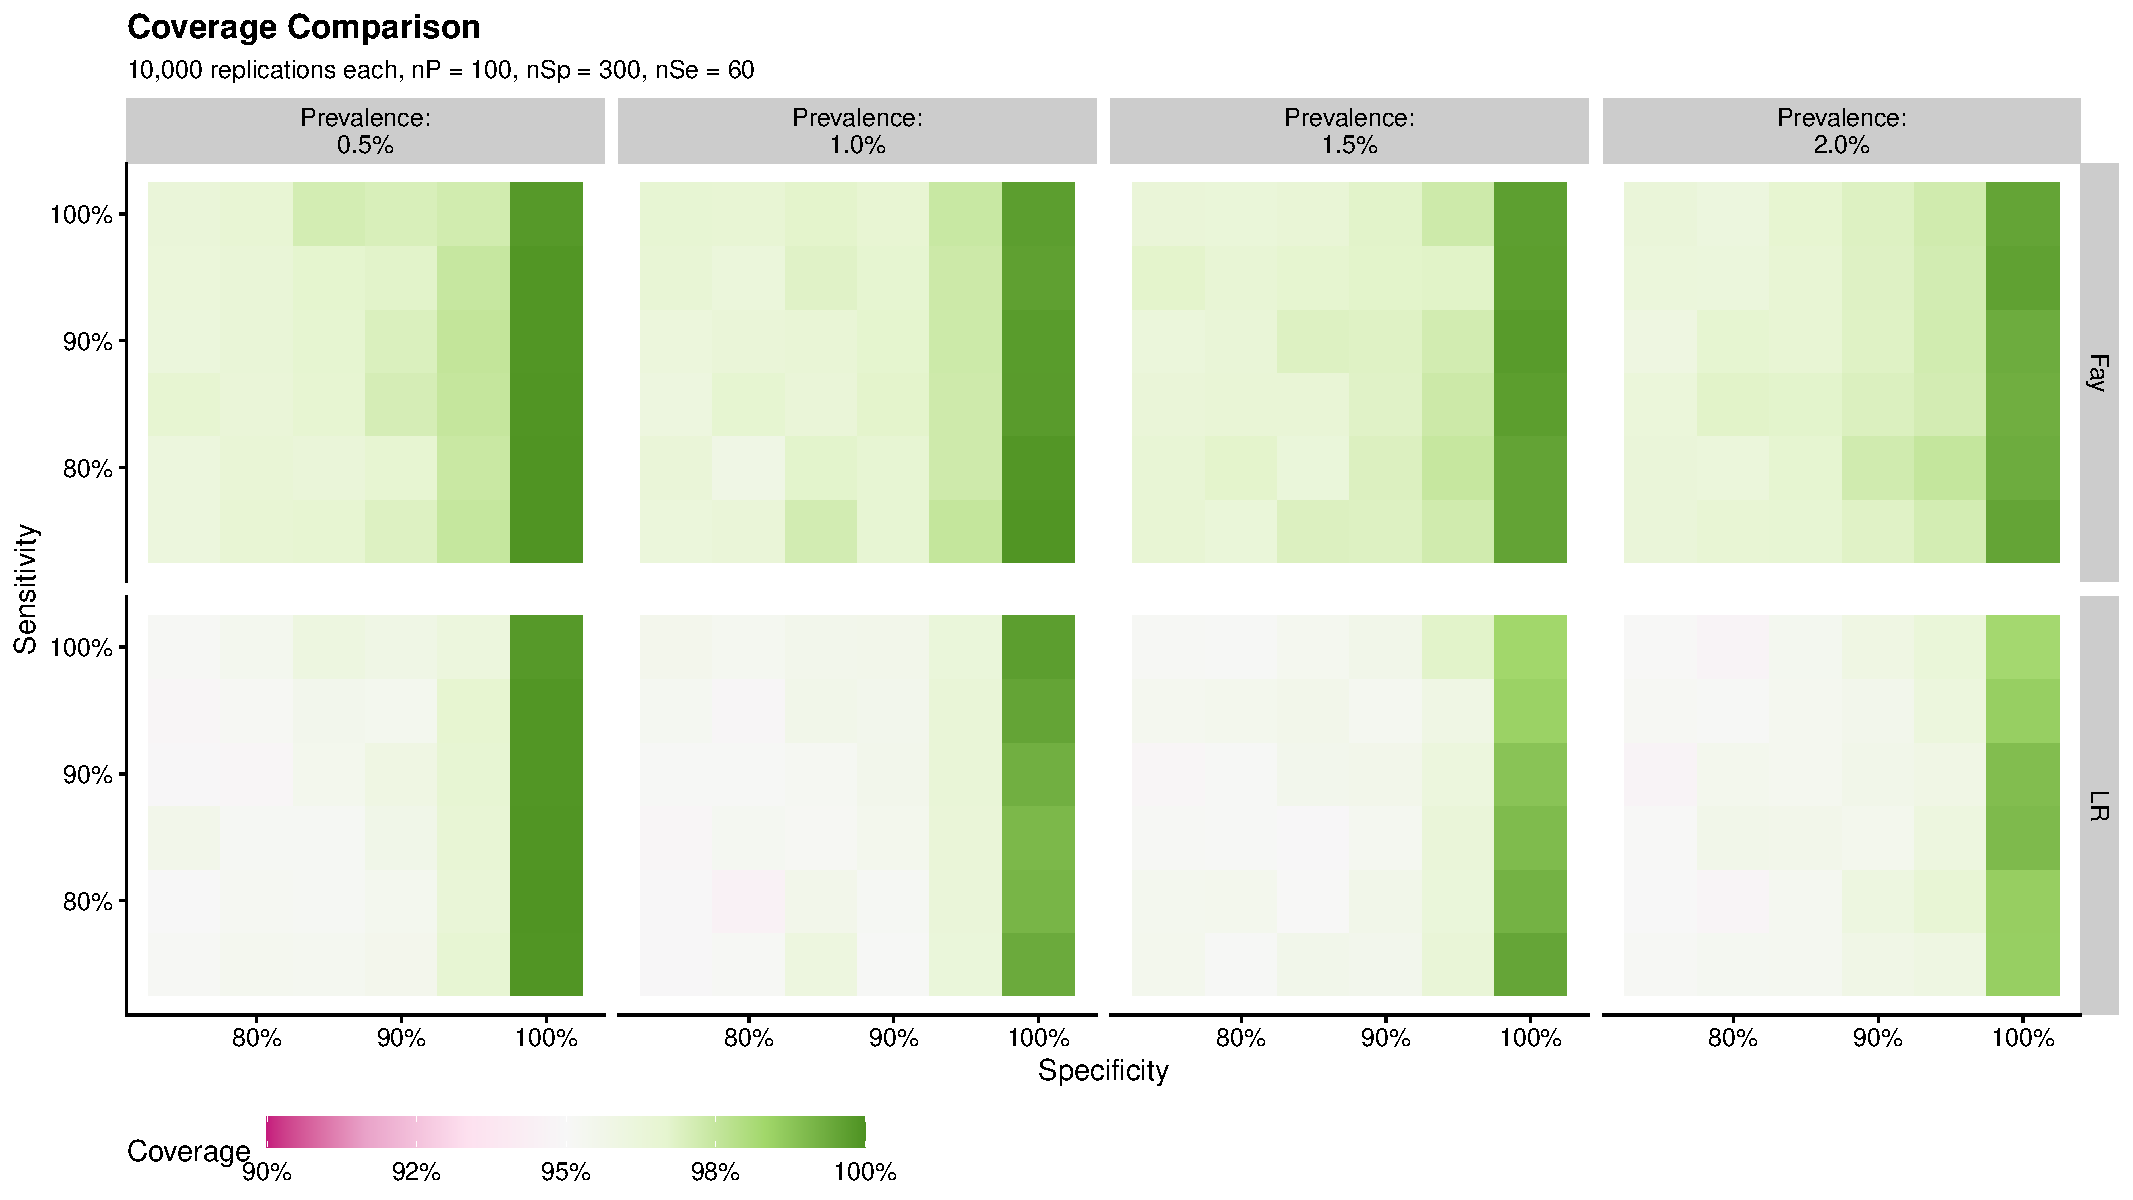
\includegraphics[width=\textwidth]{figures/coverage_comparison_plot}
    \caption{Coverage properties for our new method (Fay) and the state of the art method (LR) in a variety of settings, each simulated 10,000 times.}
    \label{fig:coverage_comparison_plot}
\end{figure}

\begin{figure}
    \centering
    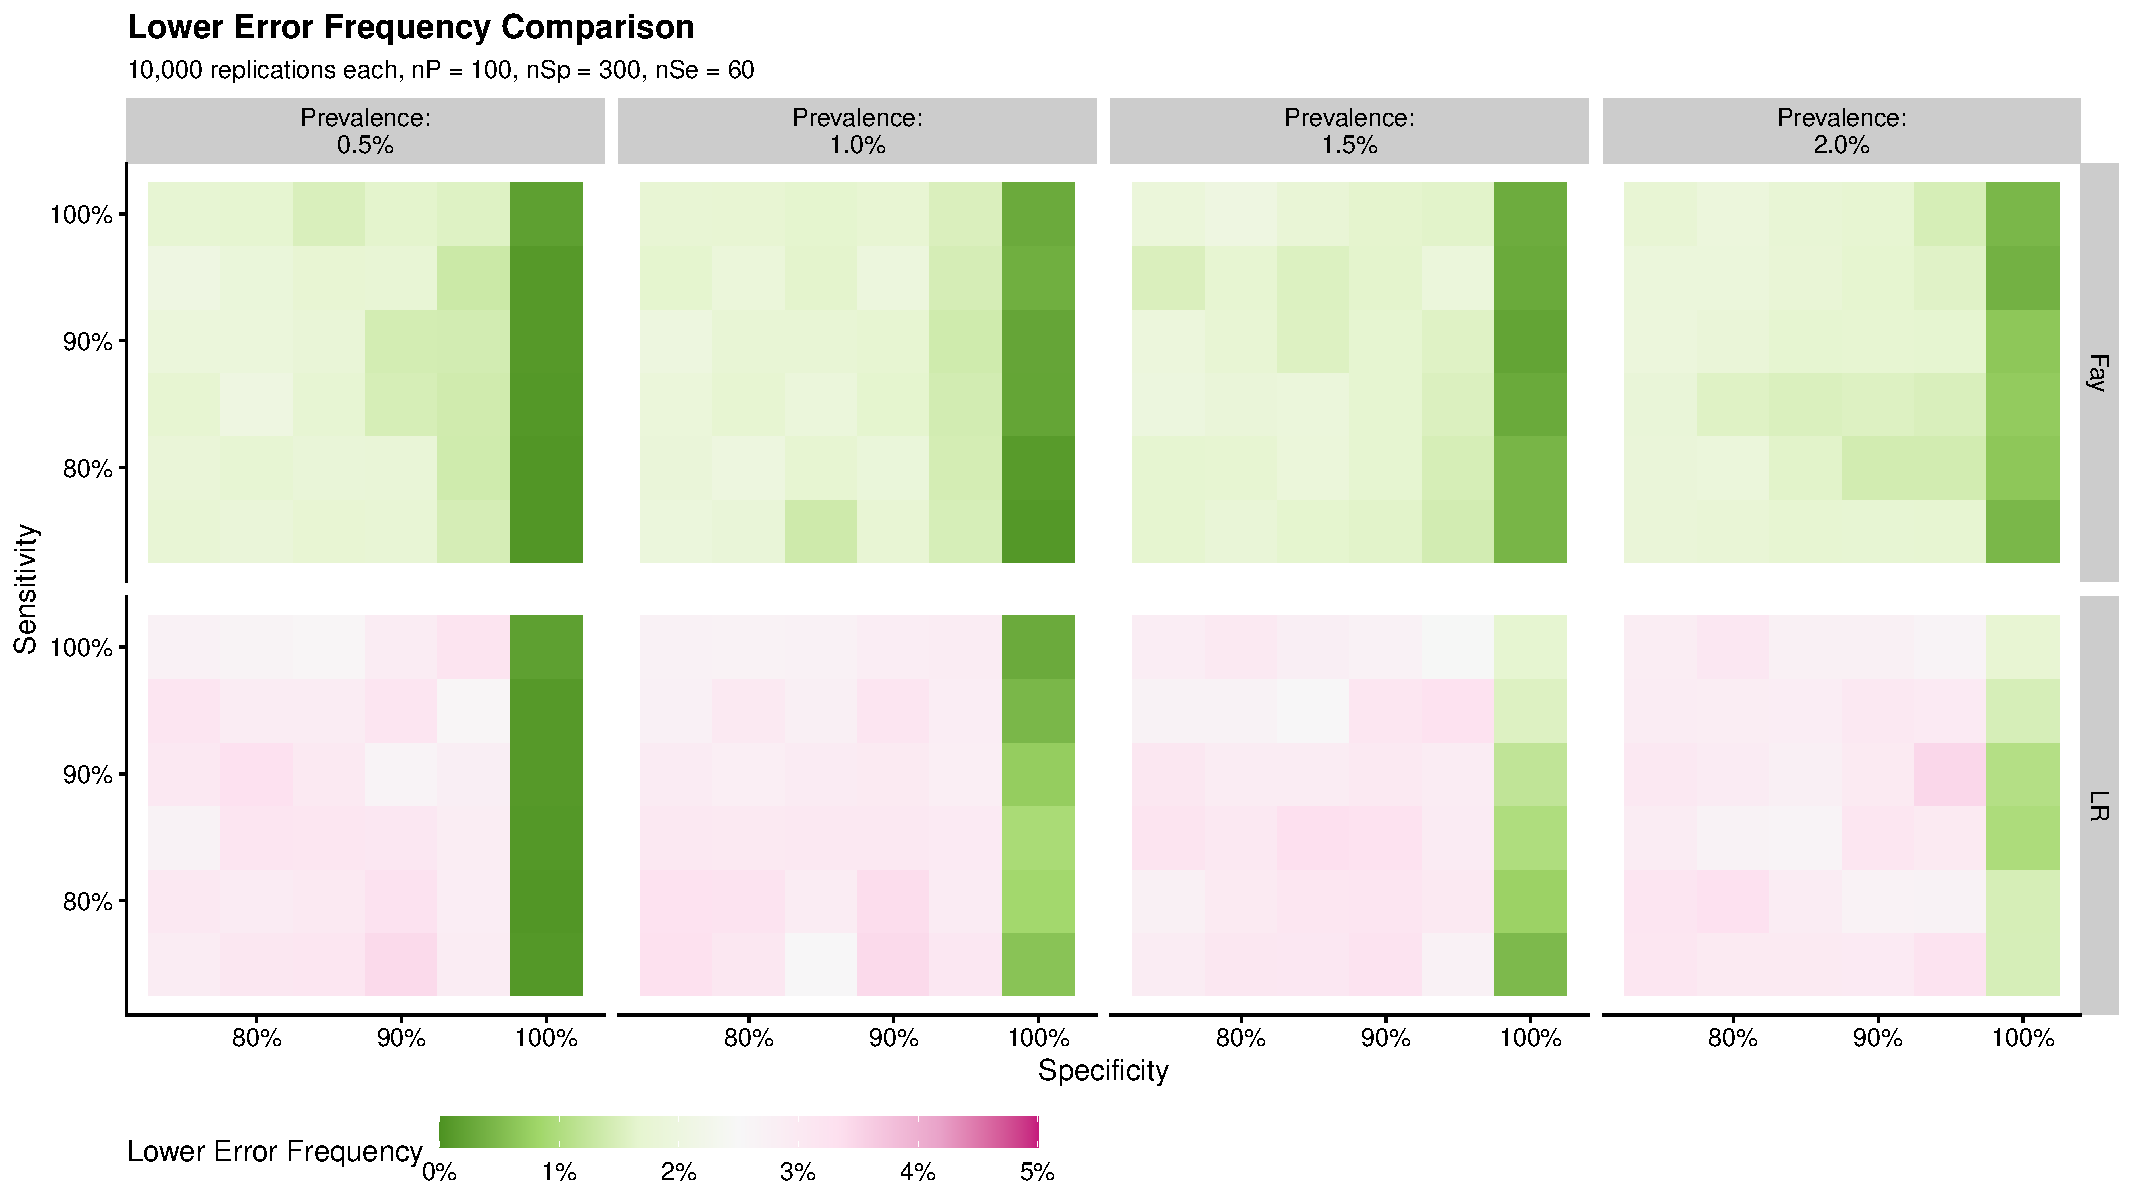
\includegraphics[width=\textwidth]{figures/lower_error_frequency_comparison_plot}
    \caption{Lower error properties for our new method (Fay) and the state of the art method (LR) in a variety of settings, each simulated 10,000 times.}
    \label{fig:lower_error_frequency_comparison_plot}
\end{figure}

\begin{figure}
    \centering
    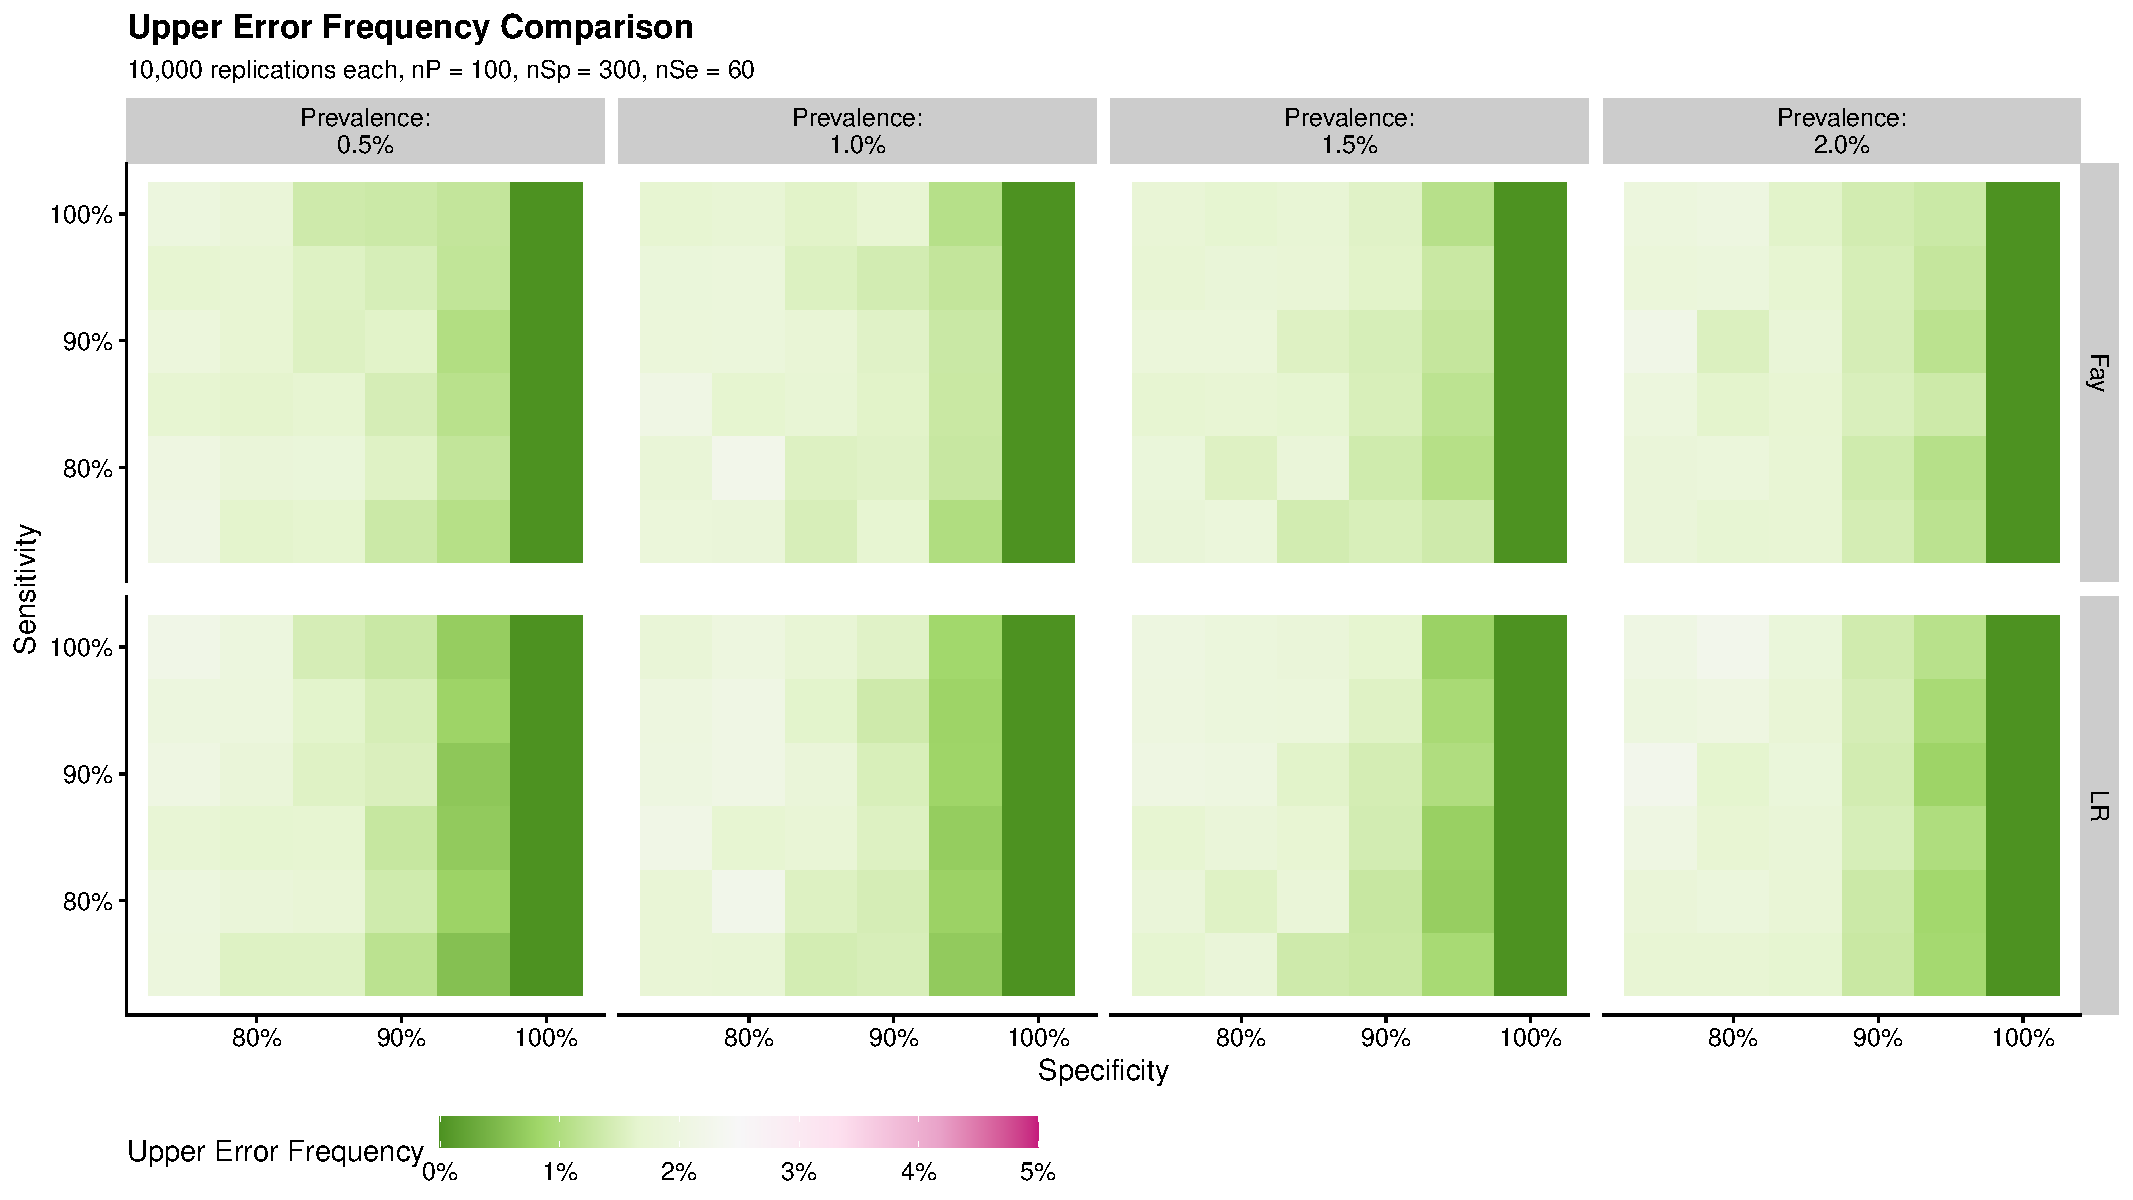
\includegraphics[width=\textwidth]{figures/upper_error_frequency_comparison_plot}
    \caption{Upper error properties for our new method (Fay) and the state of the art method (LR) in a variety of settings, each simulated 10,000 times.}
    \label{fig:upper_error_frequency_comparison_plot}
\end{figure}

\subsection{Estimating Prevalence from a Weighted Sample with a Perfect Assay}

We compare the wsPoisson method to the more traditional Agresti-Coull and Korn-Graubard methods in a variety of settings.
Our simulations examine varying levels of disease prevalence (0.5\% or 5\%), types of groups surveyed (50 groups 200 subjects or 8000 groups of 1 subject), distributions of weights among the groups (coefficient of variation from 0-6), the number of groups with non-zero prevalence, and the weights of the groups with non-zero prevalence.
For each scenario, 10,000 data sets are simulated and assessed.

The coverage properties for these simulations are presented in Figures~\ref{fig:perfect_coverage_50_0_005_reduced}--\ref{fig:perfect_coverage_8000_0_05_reduced.pdf}.

\begin{figure}
    \centering
    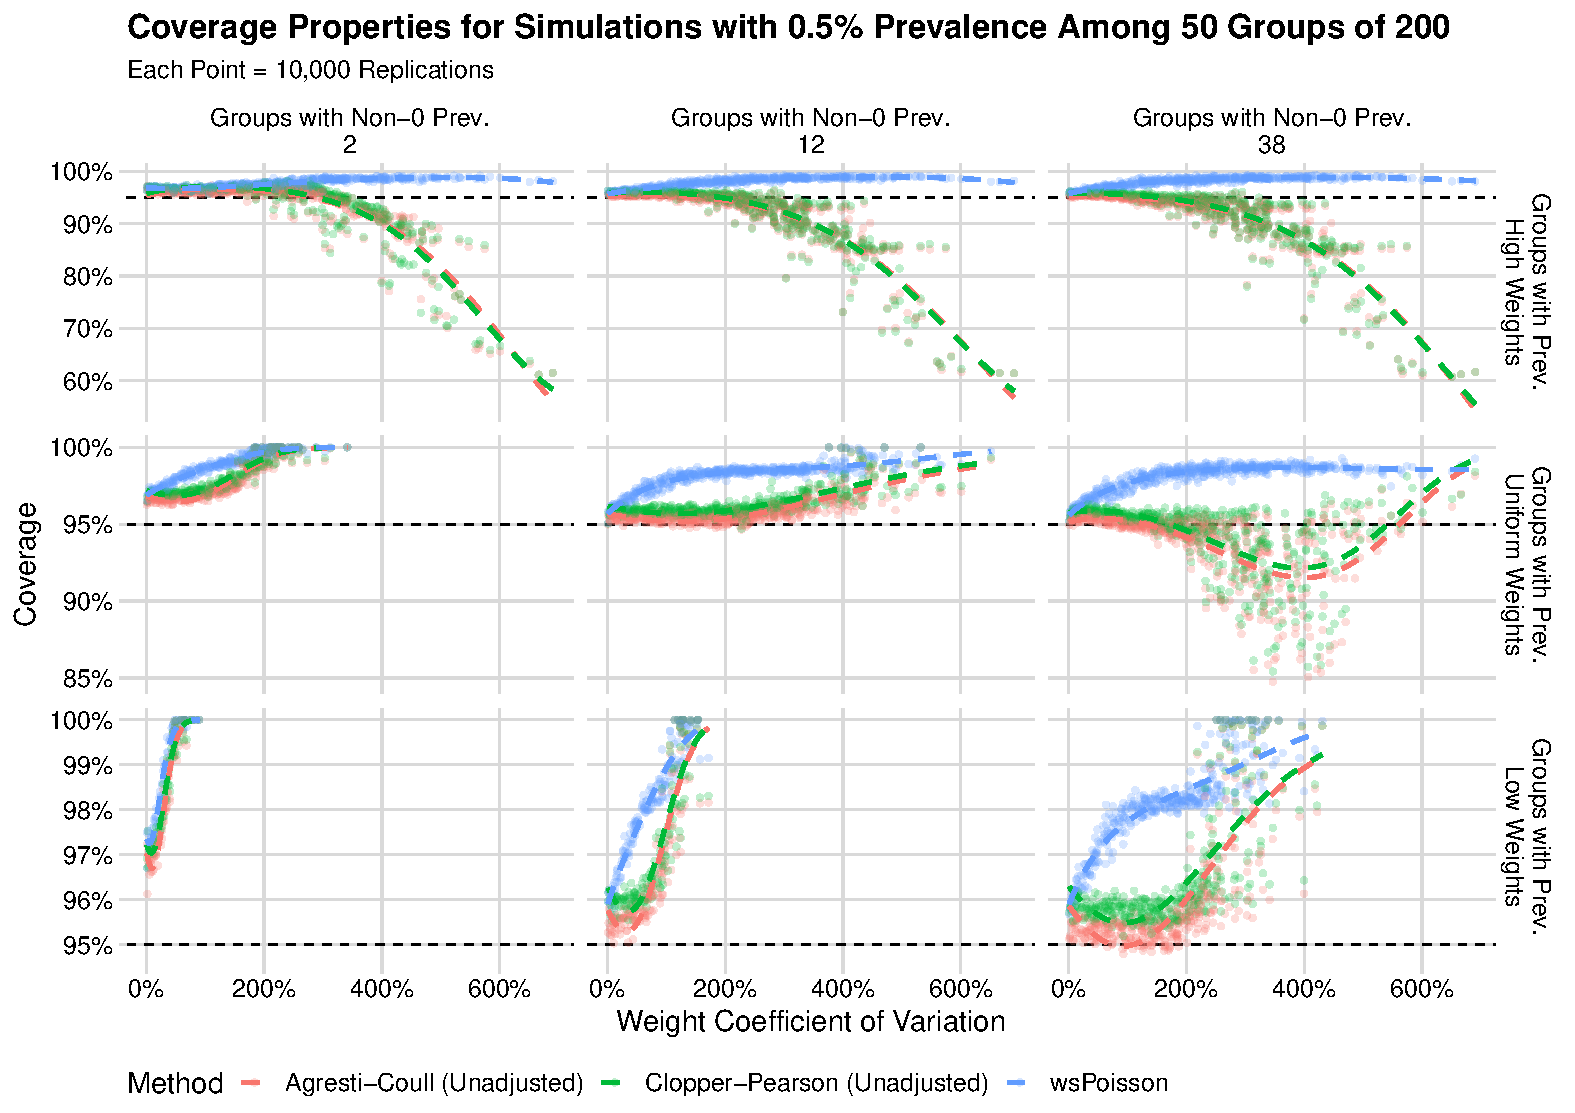
\includegraphics[width=\textwidth]{figures/perfect_coverage_50_0_005_reduced.pdf}
    \caption{Caption}
    \label{fig:perfect_coverage_50_0_005_reduced}
\end{figure}


\begin{figure}
    \centering
    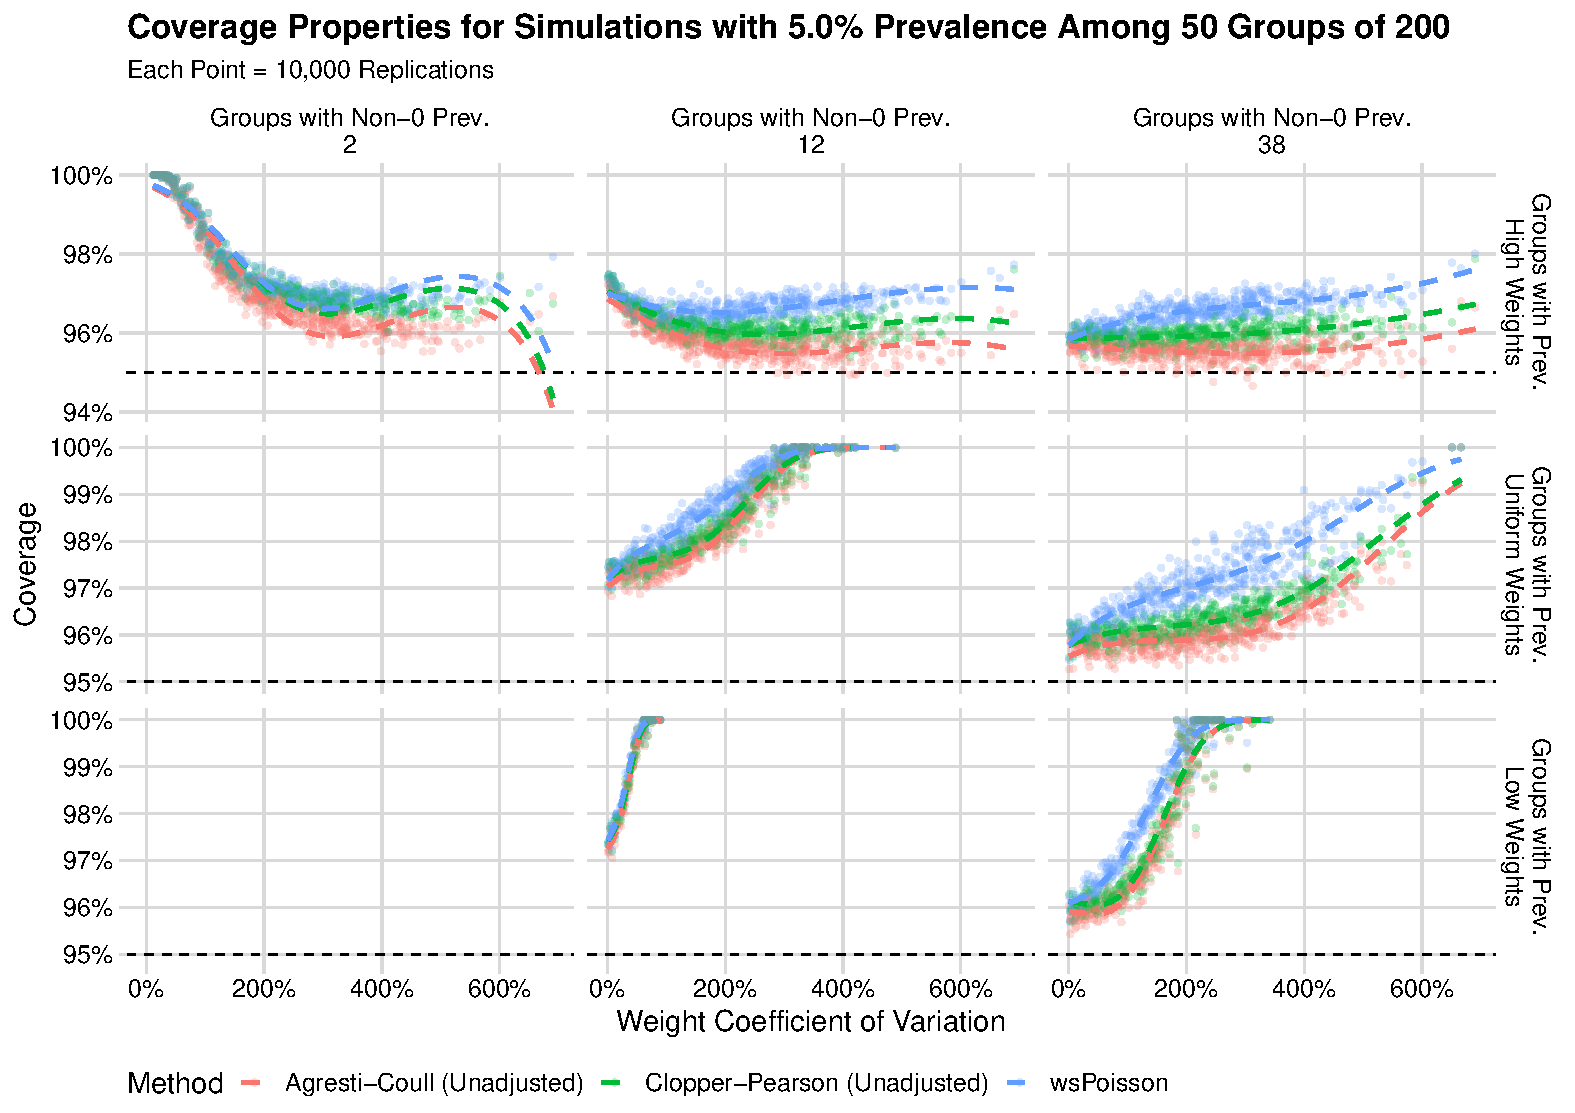
\includegraphics[width=\textwidth]{figures/perfect_coverage_50_0_05_reduced.pdf}
    \caption{Caption}
    \label{fig:perfect_coverage_50_0_05_reduced}
\end{figure}


\begin{figure}
    \centering
    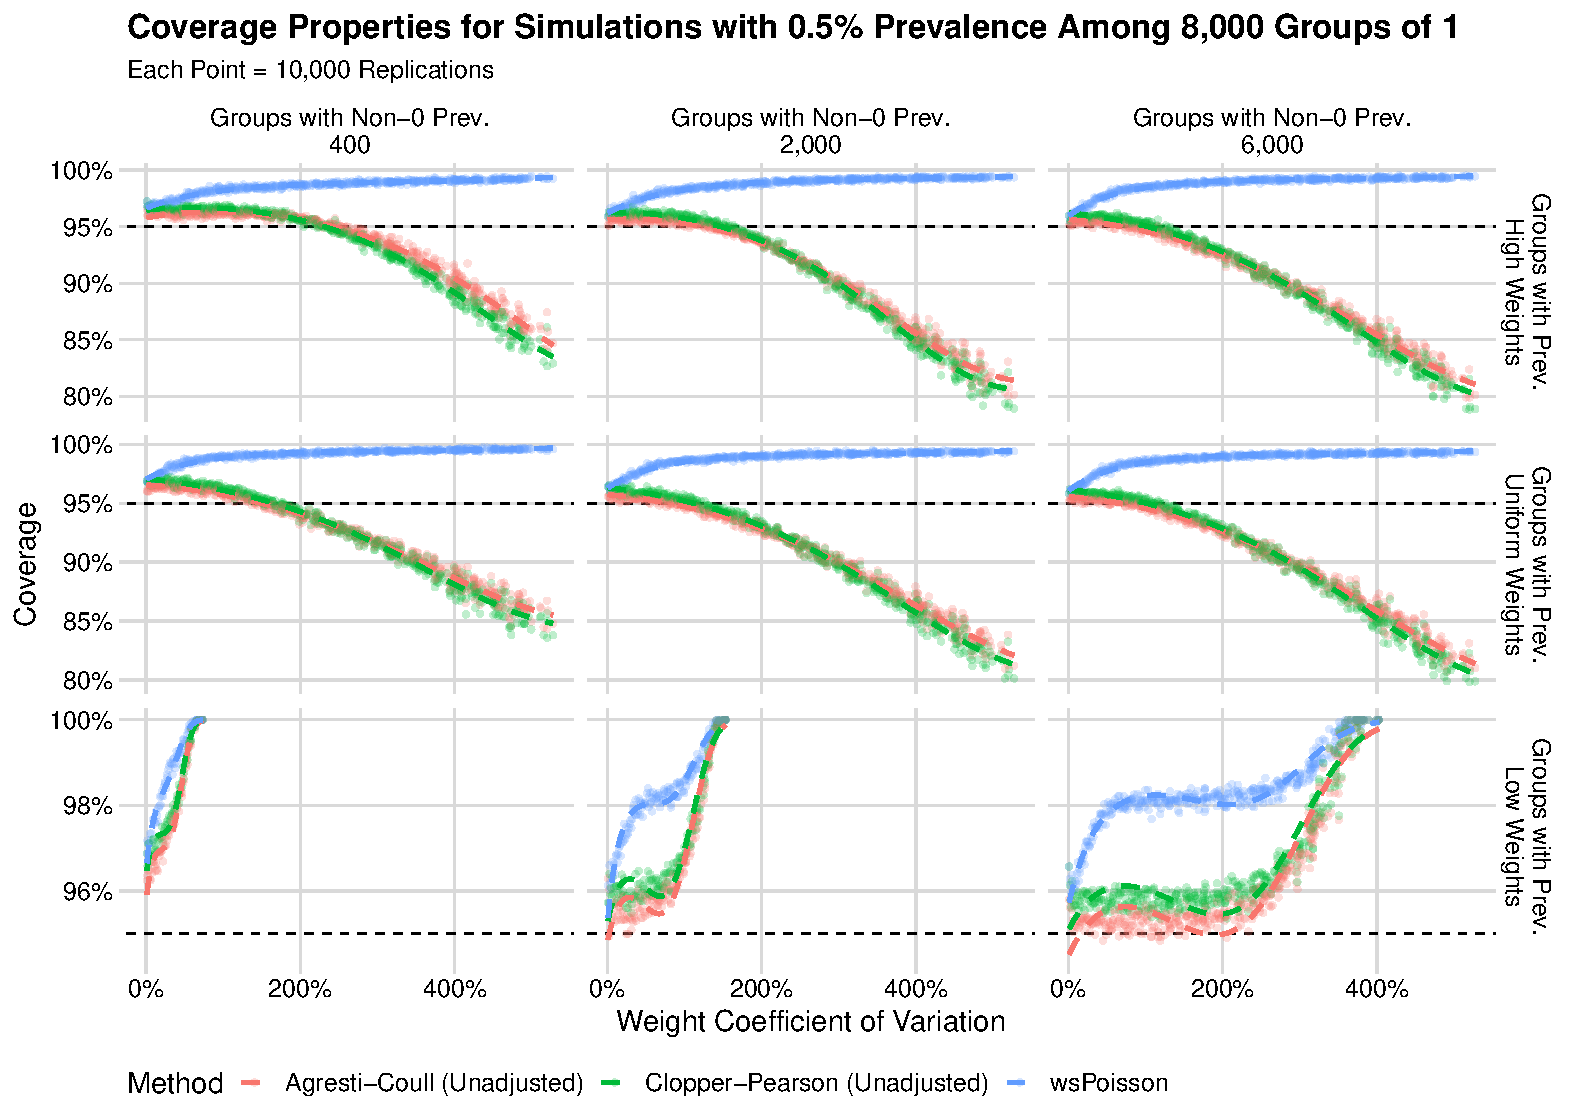
\includegraphics[width=\textwidth]{figures/perfect_coverage_8000_0_005_reduced.pdf}
    \caption{Caption}
    \label{fig:perfect_coverage_8000_0_005_reduced}
\end{figure}

\begin{figure}
    \centering
    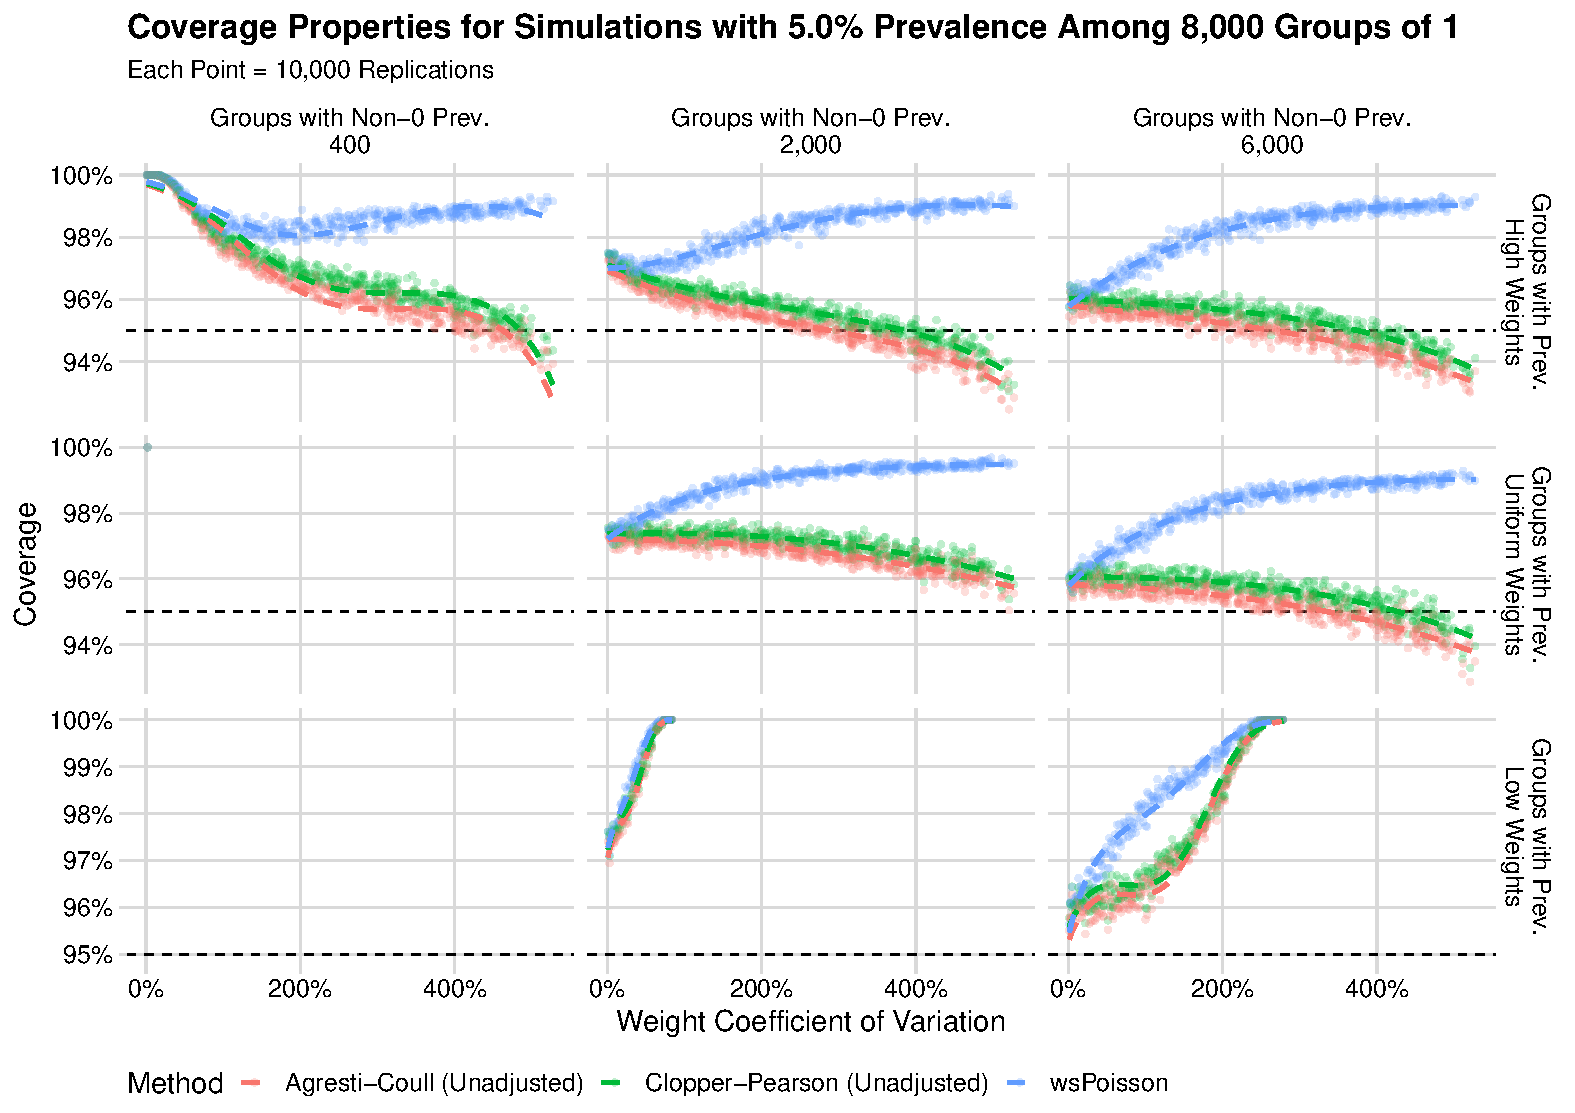
\includegraphics[width=\textwidth]{figures/perfect_coverage_8000_0_05_reduced.pdf}
    \caption{Caption}
    \label{fig:perfect_coverage_8000_0_05_reduced.pdf}
\end{figure}



\subsection{Estimating Prevalence from a Weighted Sample with an Imperfect Assay}
\todo[inline]{THERE IS A SMALL ERROR IN THE SIMULATION RESULTS. RERUNNING ON BIOWULF NOW. I DON'T EXPECT THE SUBSTANCE TO CHANGE.}

We also apply these two methods to a real data set from \cite{Kali:2021}.
This data set was collected to estimate seroprevalence of SARS-CoV-2 in the United States between May and July 2020.
First we apply the methods to the full data set (\( n =  8058, \text{weight coefficient of variation} = 252\%\)).
The Korn and Graubard type confidence distributions produce the 95\% confidence interval for population prevalence (2.53\%, 6.68\%), while the wsPoisson type confidence distributions produce the 95\% confidence interval (2.56\%, "7.54\%).

We also apply the methods to the subset of only hispanic participants (\( n = 1281, \text{weight coefficient of variation} = 306\% \)).
The Korn and Graubard type confidence distributions produce the 95\% confidence interval for population prevalence (2.35\%, 11.75\%), while the wsPoisson type confidence distributions produce the 95\% confidence interval (2.40\%, 20.02\%).
\todo[inline] Maybe also compute with the non sensitivity/specificity adjusted interval.

\begin{figure}
    \centering
    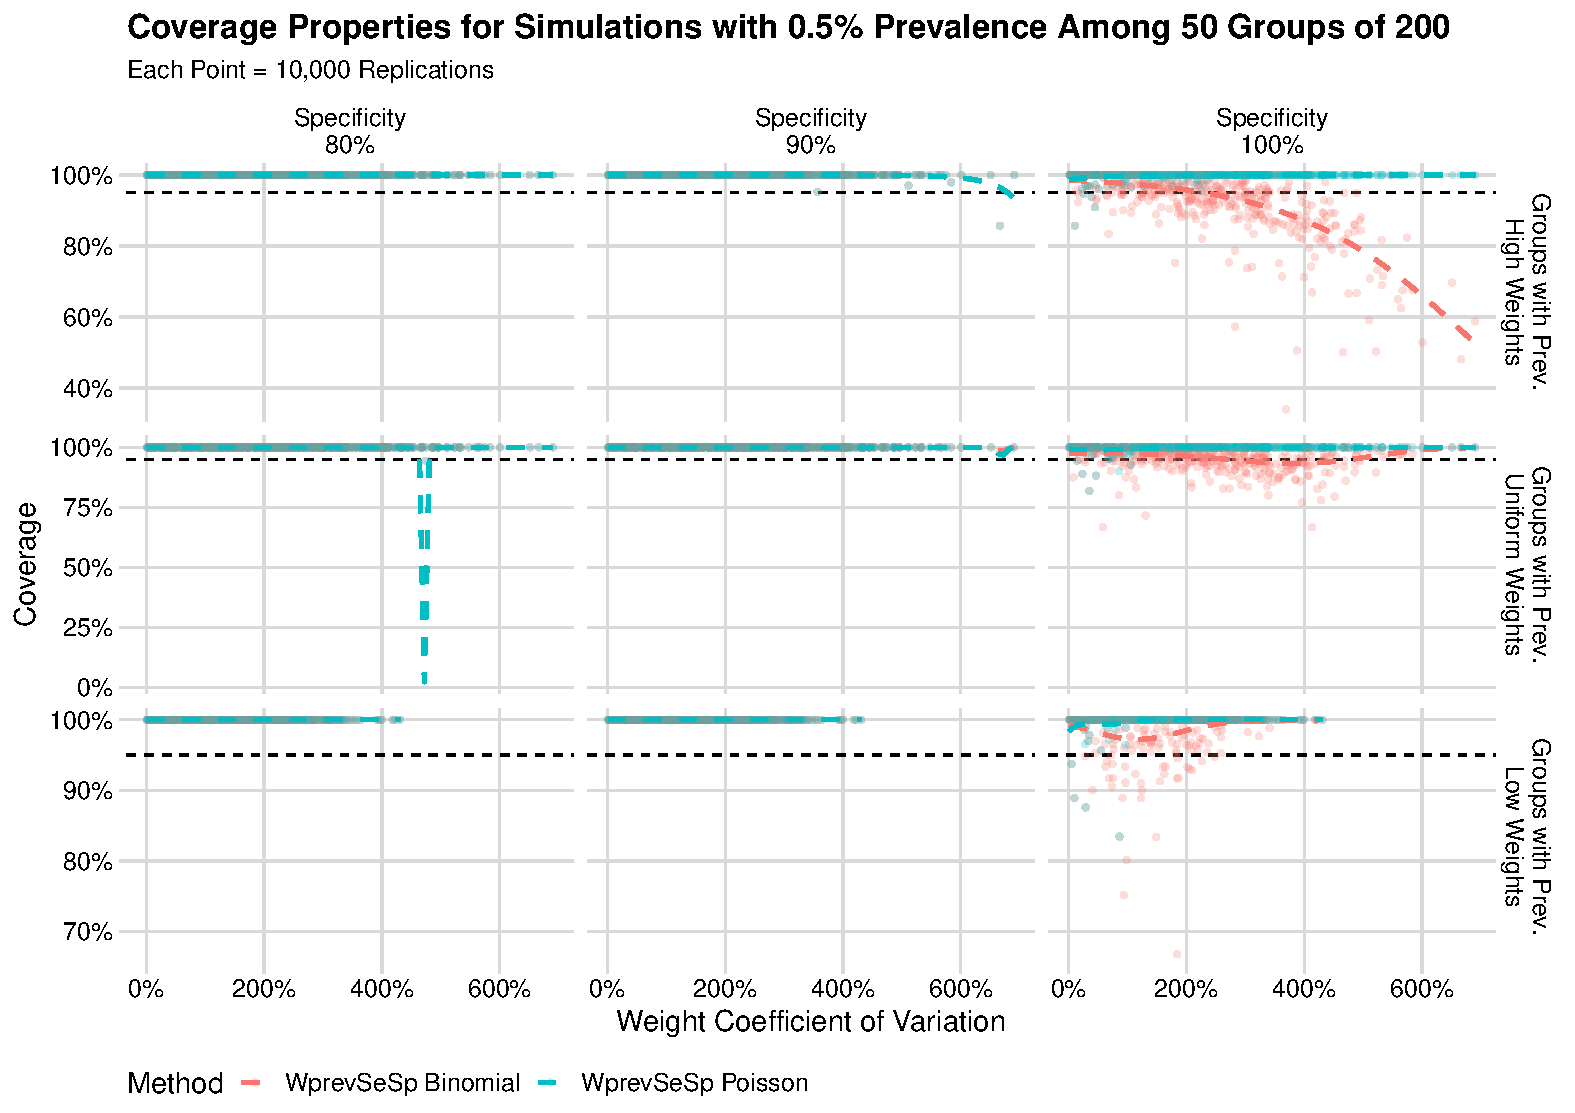
\includegraphics[width=\textwidth]{figures/imperfect_coverage_50_0_005_reduced.pdf}
    \caption{Caption}
    \label{fig:imperfect_coverage_50_0_005_reduced}
\end{figure}


\begin{figure}
    \centering
    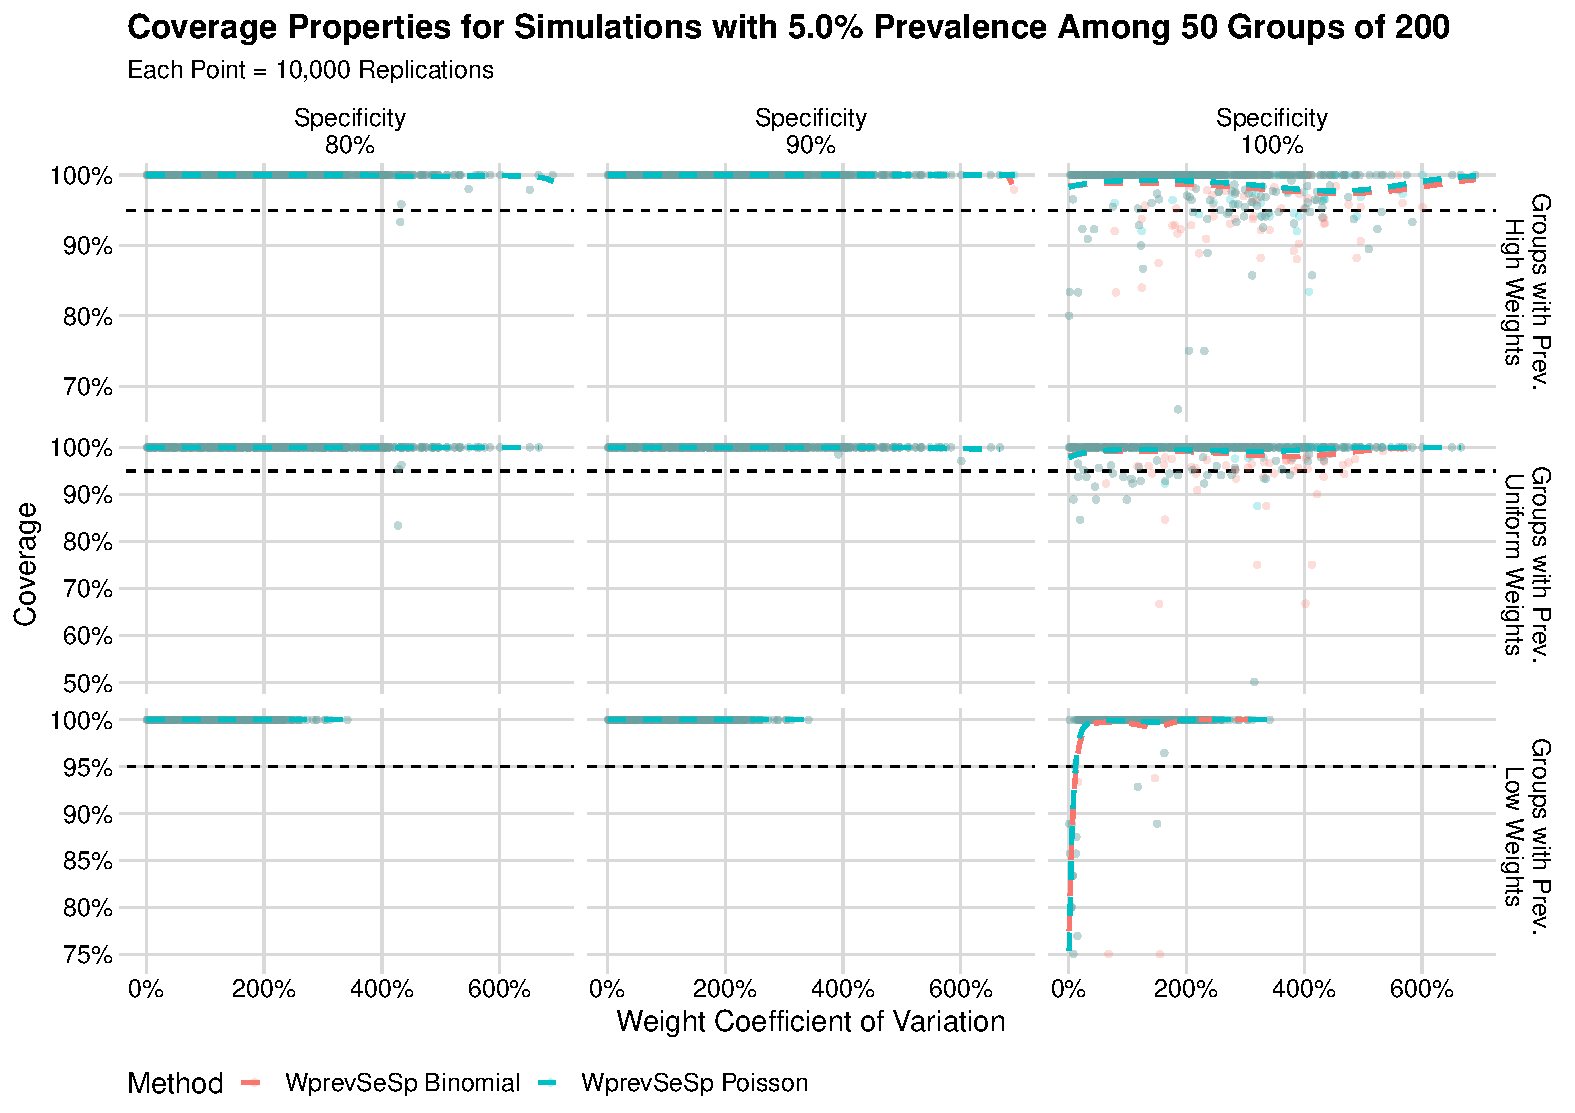
\includegraphics[width=\textwidth]{figures/imperfect_coverage_50_0_05_reduced.pdf}
    \caption{Caption}
    \label{fig:imperfect_coverage_50_0_05_reduced}
\end{figure}


\begin{figure}
    \centering
    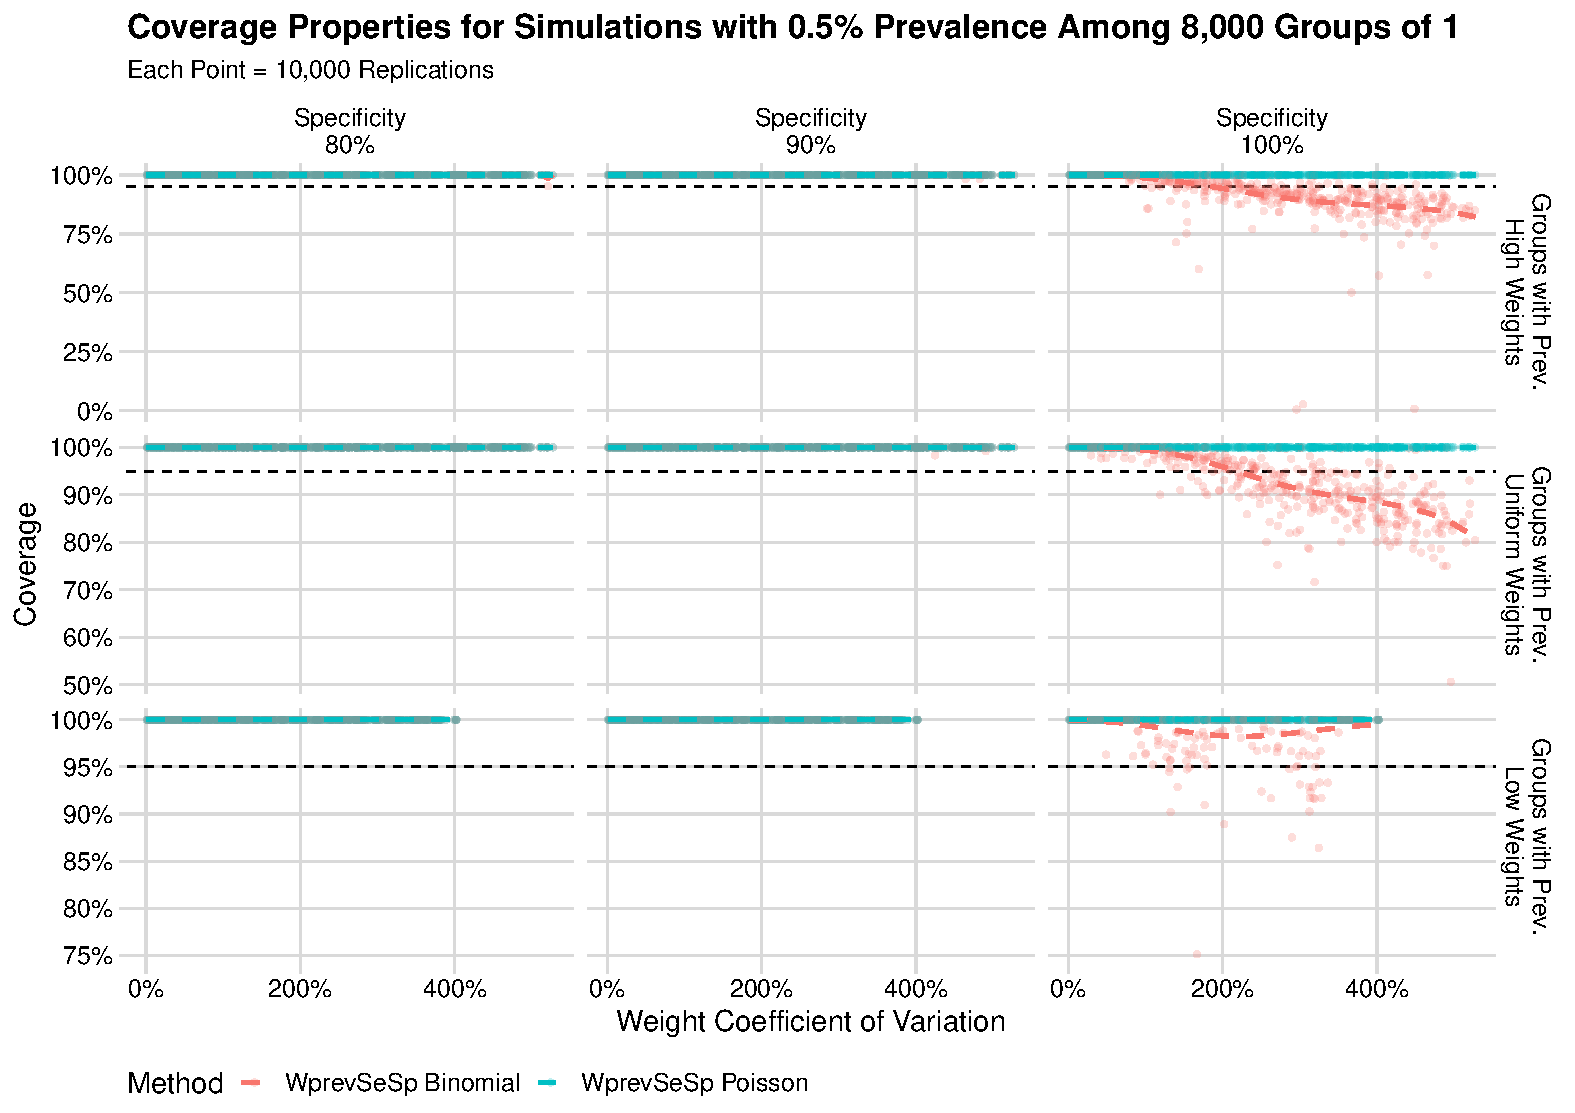
\includegraphics[width=\textwidth]{figures/imperfect_coverage_8000_0_005_reduced.pdf}
    \caption{Caption}
    \label{fig:imperfect_coverage_8000_0_005_reduced}
\end{figure}

\begin{figure}
    \centering
    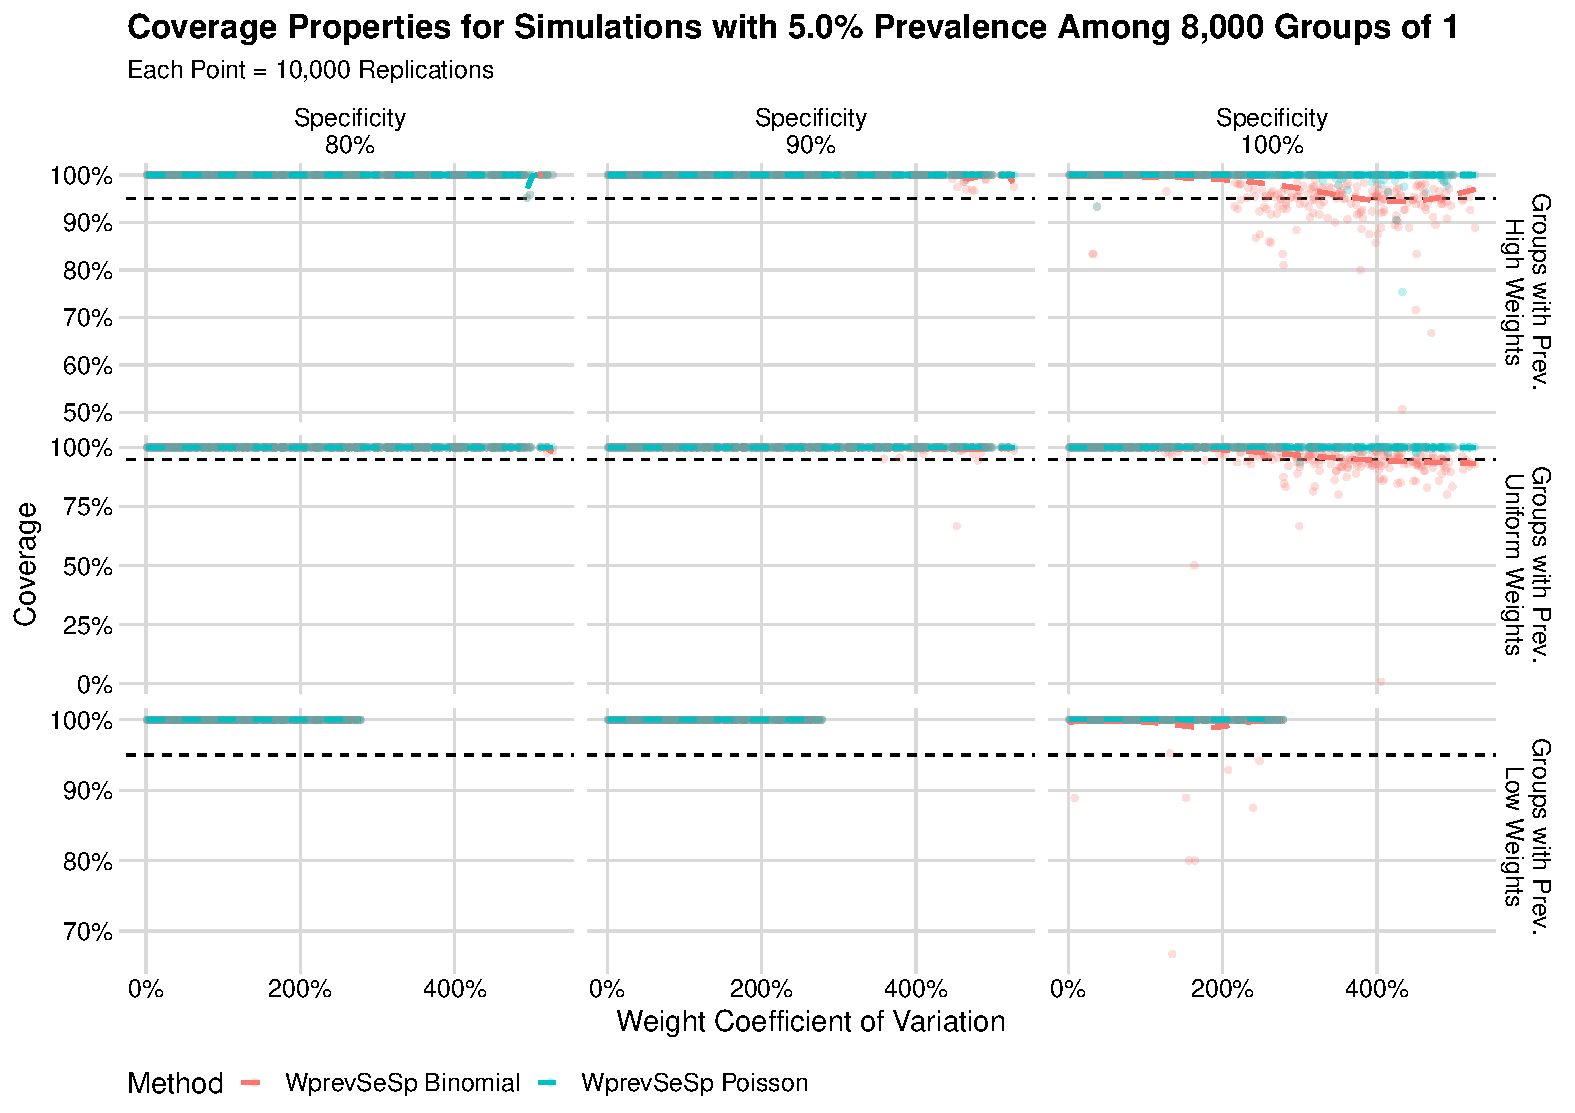
\includegraphics[width=\textwidth]{figures/imperfect_coverage_8000_0_05_reduced.pdf}
    \caption{Caption}
    \label{fig:imperfect_coverage_8000_0_05_reduced.pdf}
\end{figure}




Misc quotes from Mike to incorporate:

\begin{itemize}
    \item The last time we met, you mentioned that it would be nice to report the weights in terms of coefficient of variation. I went back to the data from the COVID seroprevalence paper in undiagnosed adults, and I calculated a coefficient of variation  of 2.52 = 252\% for all 8058 individuals, and looking at subsets, I found that the Hispanics had a CV=306\%.  
    \item For some weighting for surveys to adjust for selection bias, the coefficient of variation may be large.  For example, the coefficient of variation of the weights (CVW) for the main estimate of seroprevalence in Kalish, et al (2021) had CVW=252\%, and it could be even larger for subsets of the population (e.g., Hispanics had CVW=306\%). 
\end{itemize}



\section{Discussion}

\acks
\begin{acks}
For sharing the data from the Kalish, et al study, we thank Matthew Memoli and the LID Clinical Studies Unit of the National Institute of Allergy and Infectious Diseases, NIH,  Kaitlyn Sadtler from the National Institute of Biomedical Imaging and Bioengineering, NIH,   Matthew Hall from the National Center for Advancing Translational Sciences, NIH, and Dominic Esposito from the Fredrick National Laboratory for Cancer Research, NCI, NIH.
\end{acks}

\section{Bibliography}
\nocite{*}% Show all bib entries - both cited and uncited; comment this line to view only cited bib entries;
\bibliography{refs}%

\appendix
\section{Additional Figures}

\begin{figure}
\centering
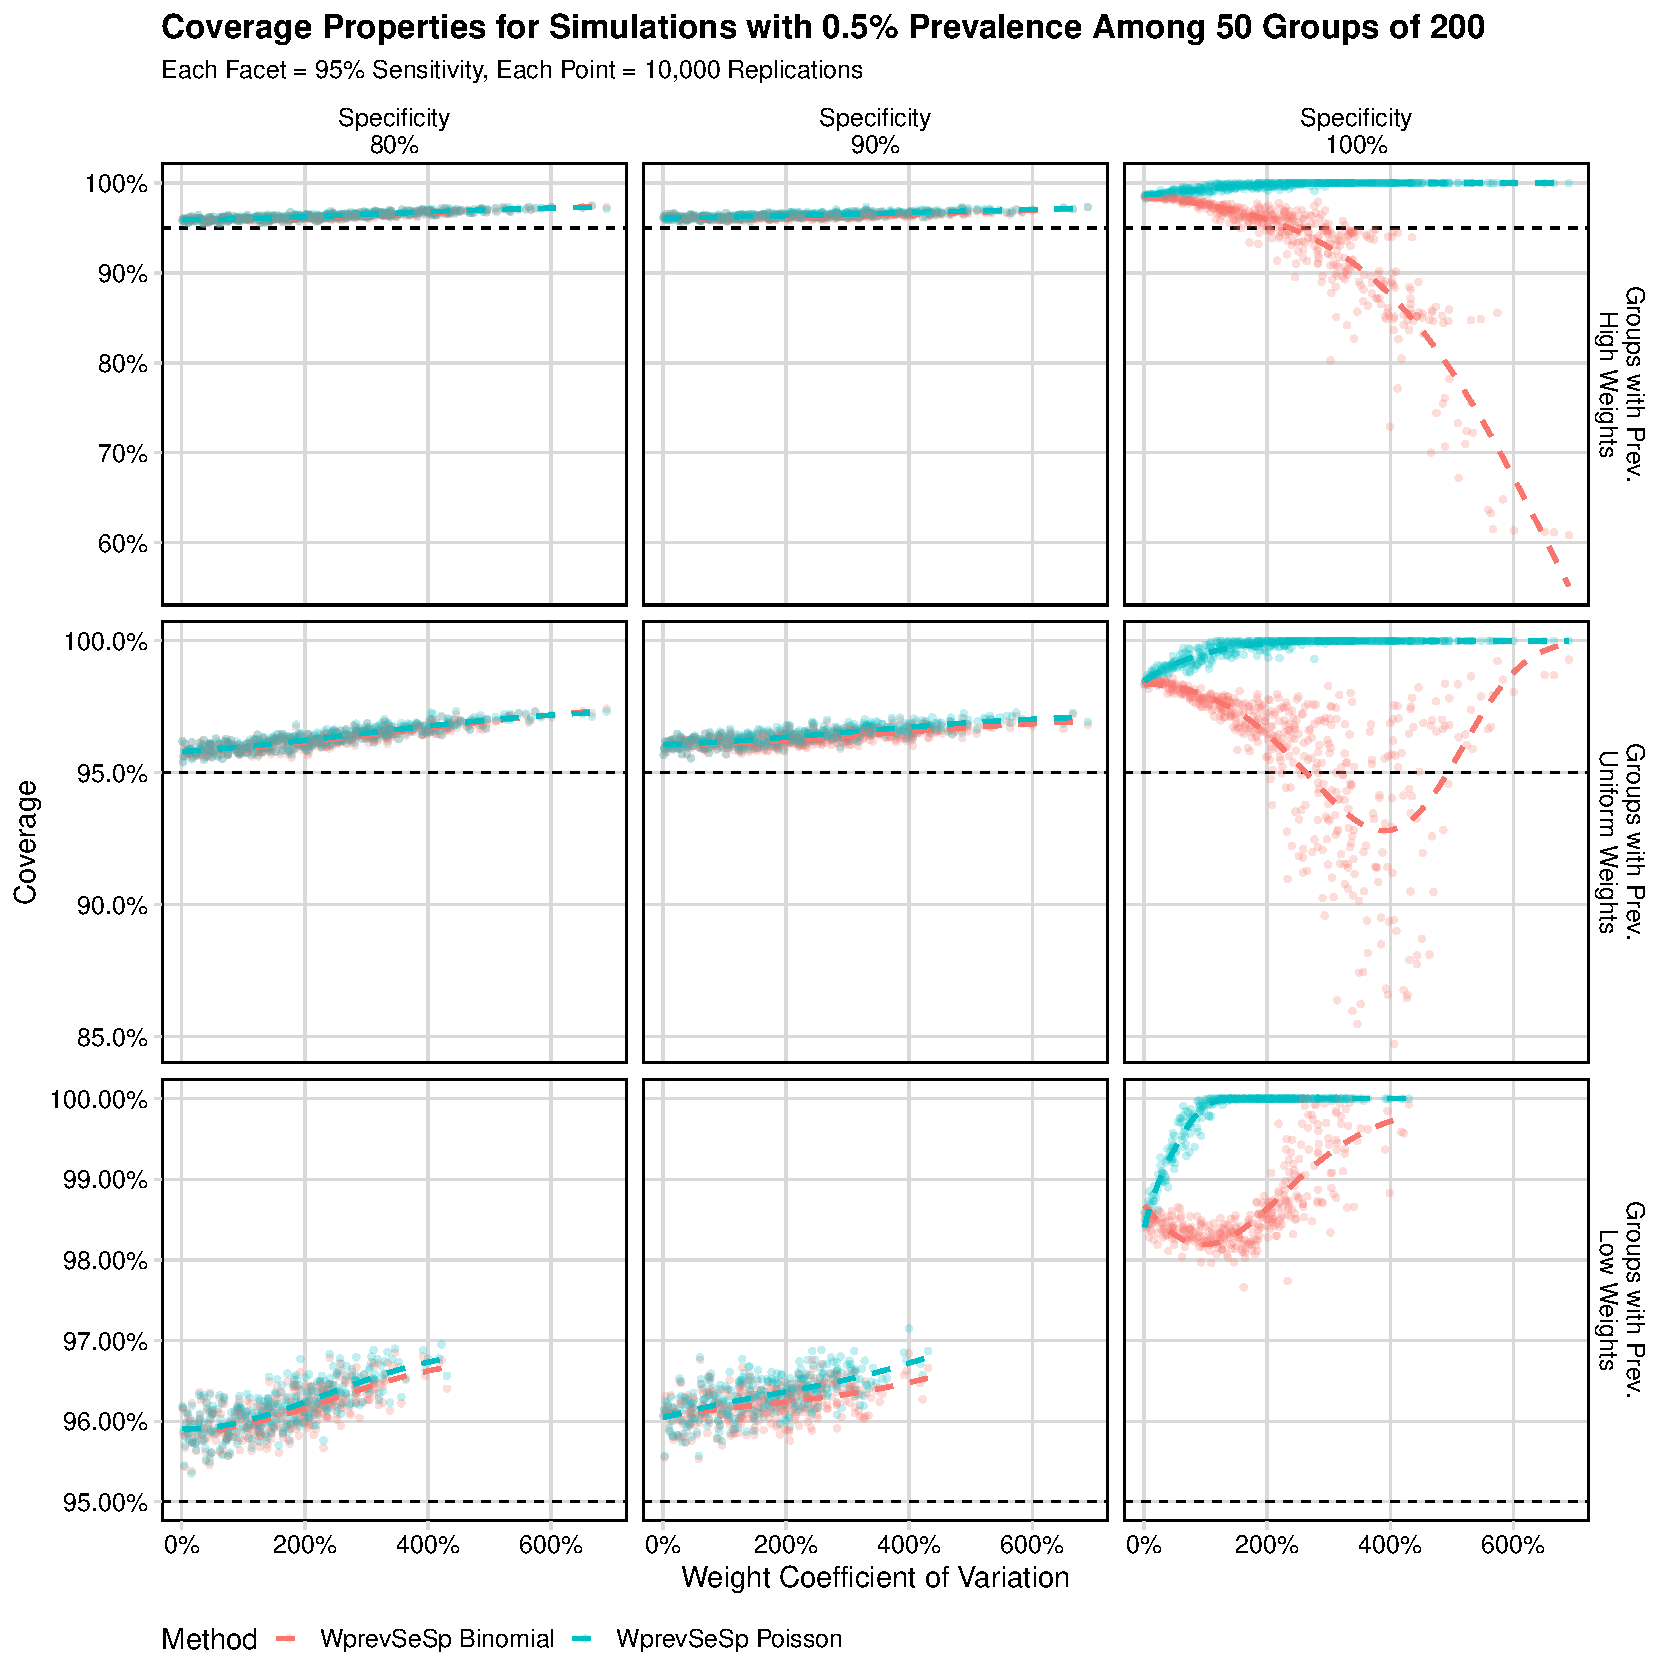
\includegraphics[width=\textwidth]{figures/imperfect_coverage_50_groups_0_005_prev.pdf}
\caption{Caption}
\label{fig:imperfect_coverage_50_groups_0_005_prev}
\end{figure}

\begin{figure}
\centering
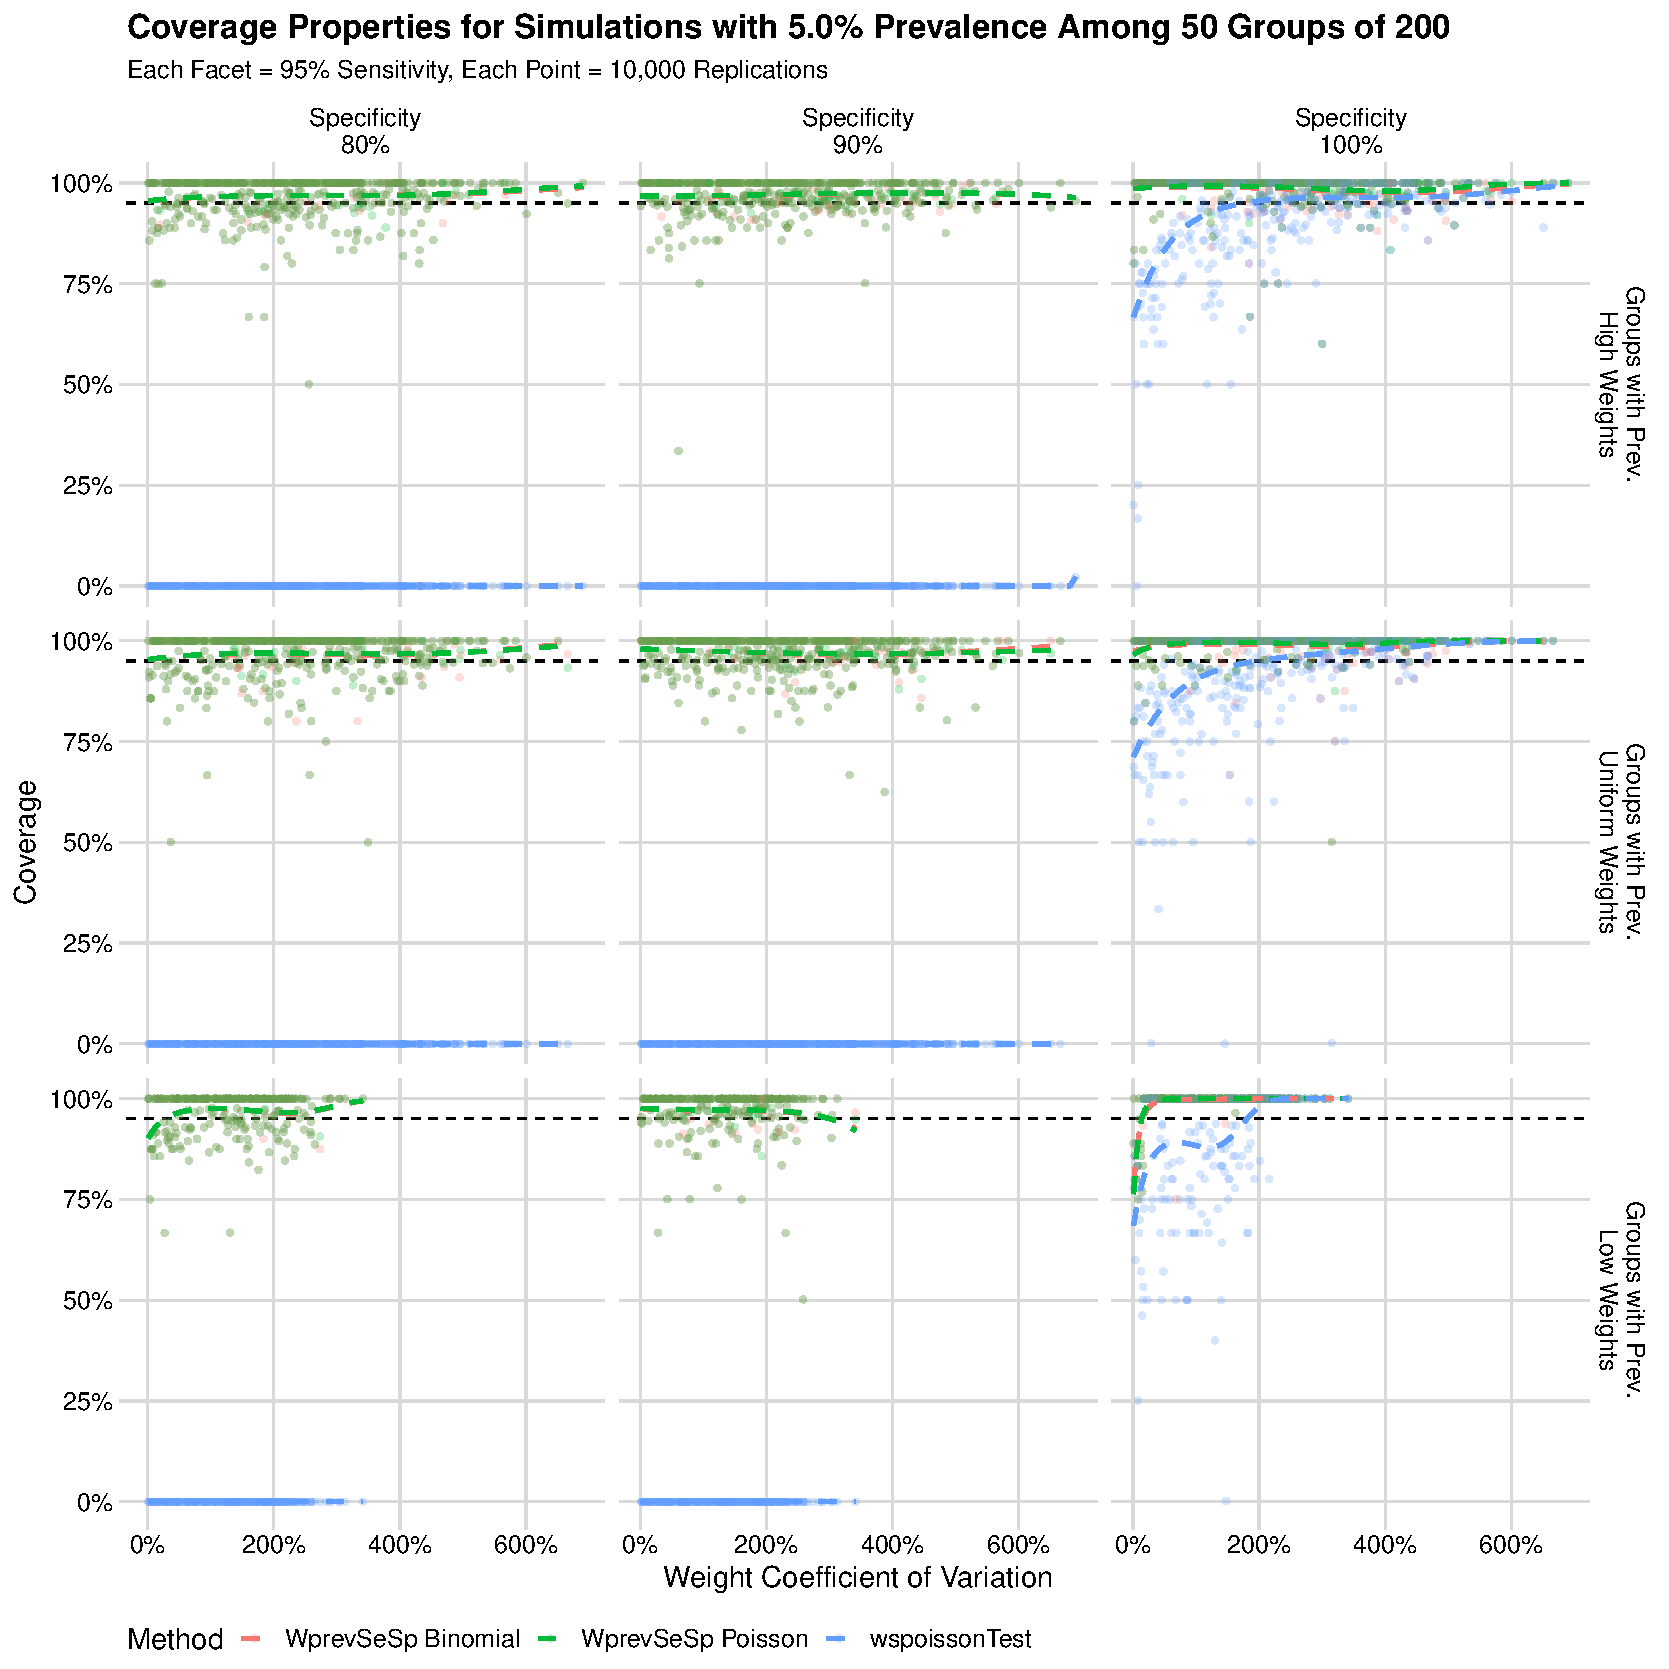
\includegraphics[width=\textwidth]{figures/imperfect_coverage_50_groups_0_05_prev.pdf}
\caption{Caption}
\label{fig:imperfect_coverage_50_groups_0_05_prev}
\end{figure}

\begin{figure}
\centering
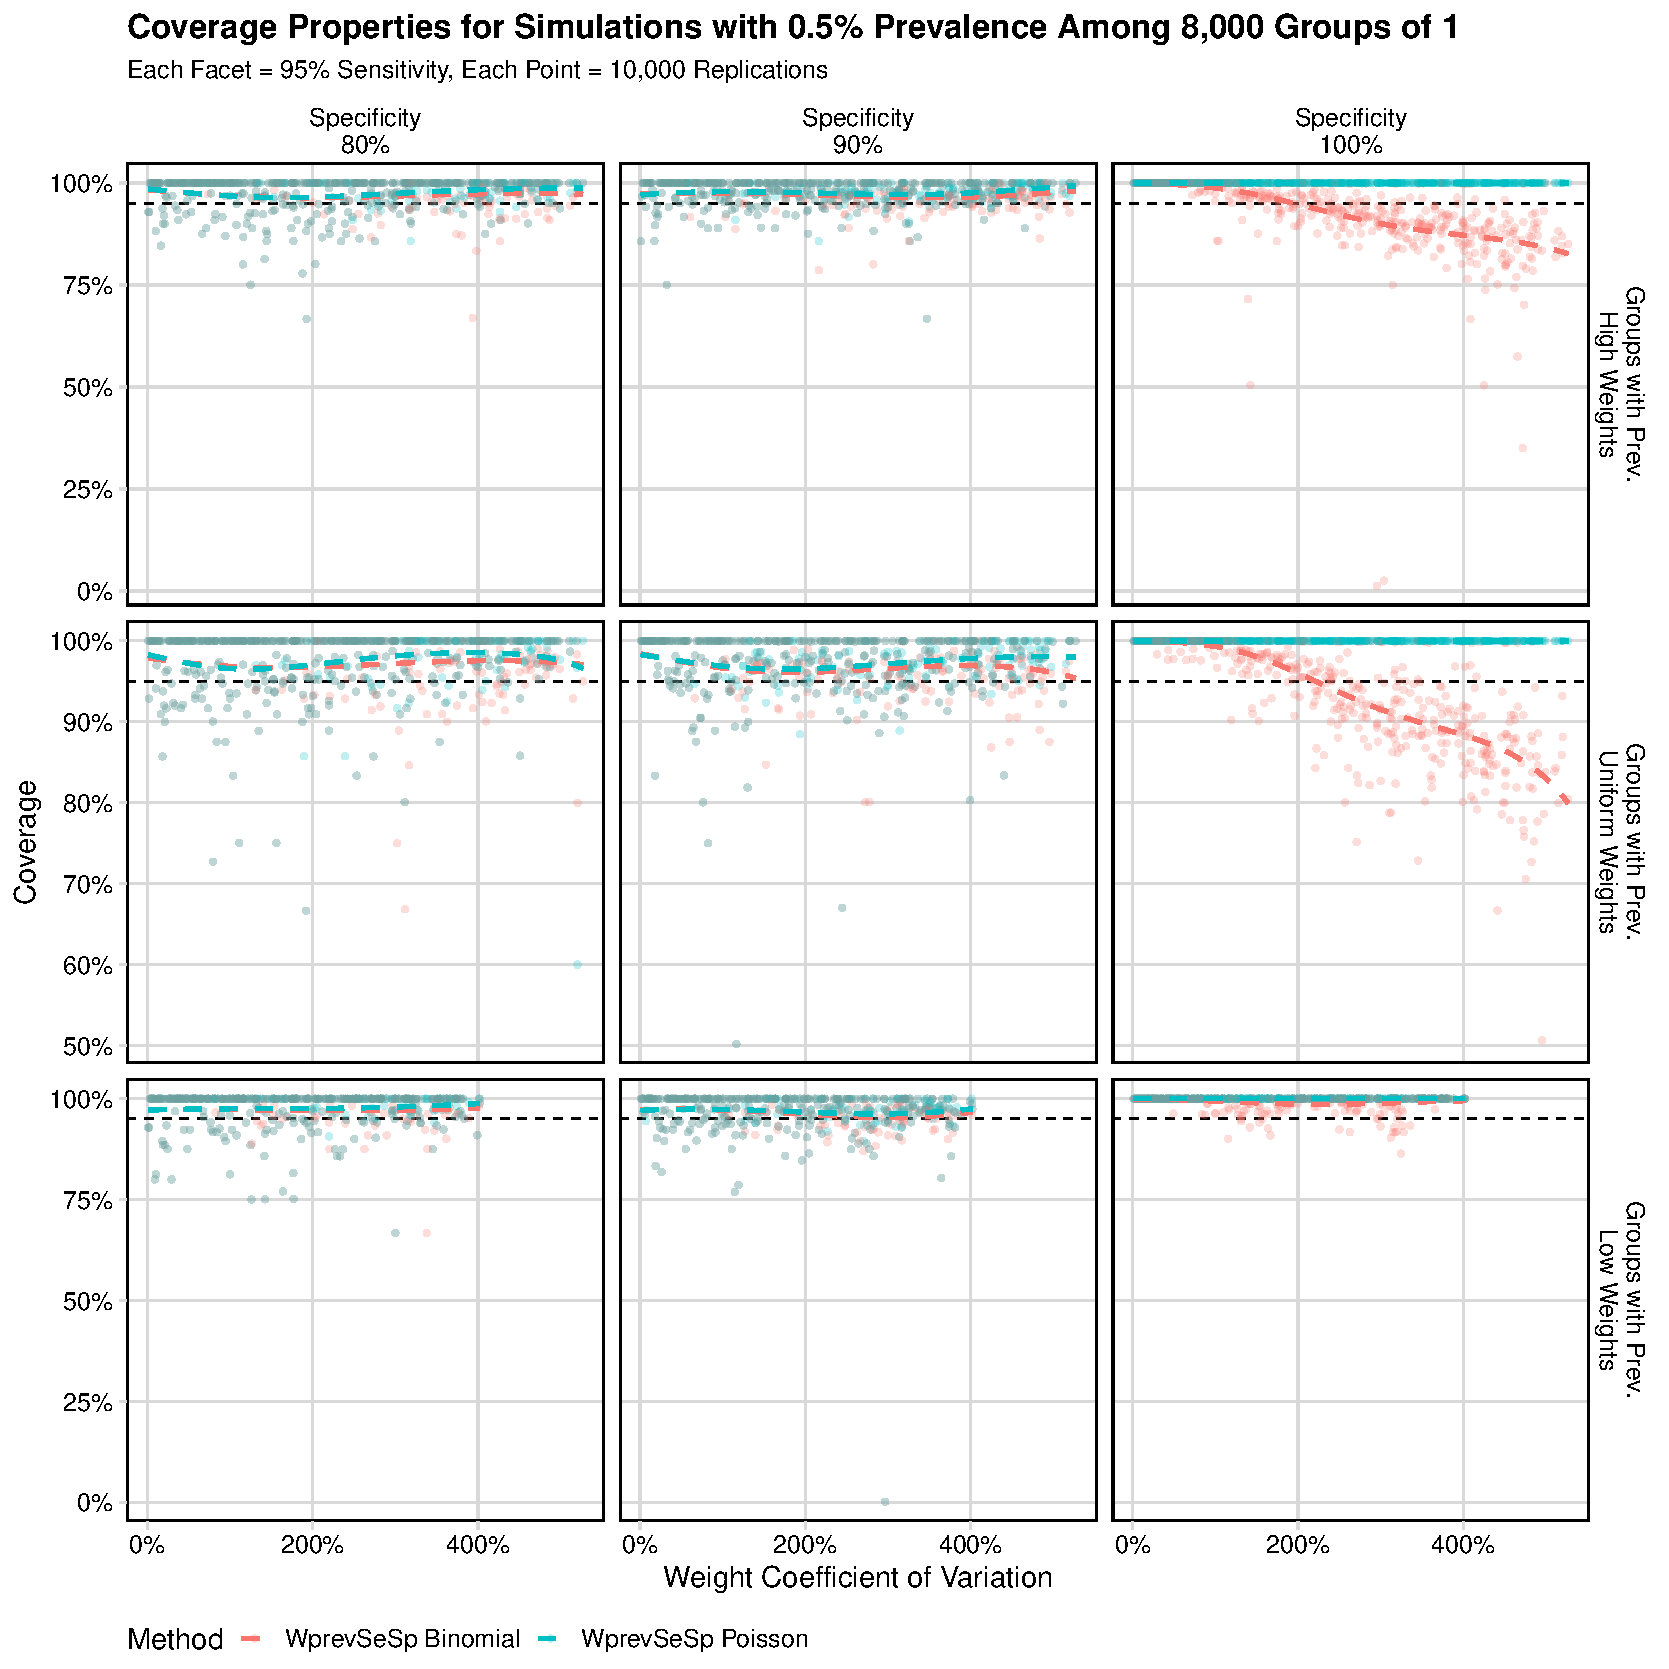
\includegraphics[width=\textwidth]{figures/imperfect_coverage_8000_groups_0_005_prev.pdf}
\caption{Caption}
\label{fig:imperfect_coverage_8000_groups_0_005_prev}
\end{figure}

\begin{figure}
\centering
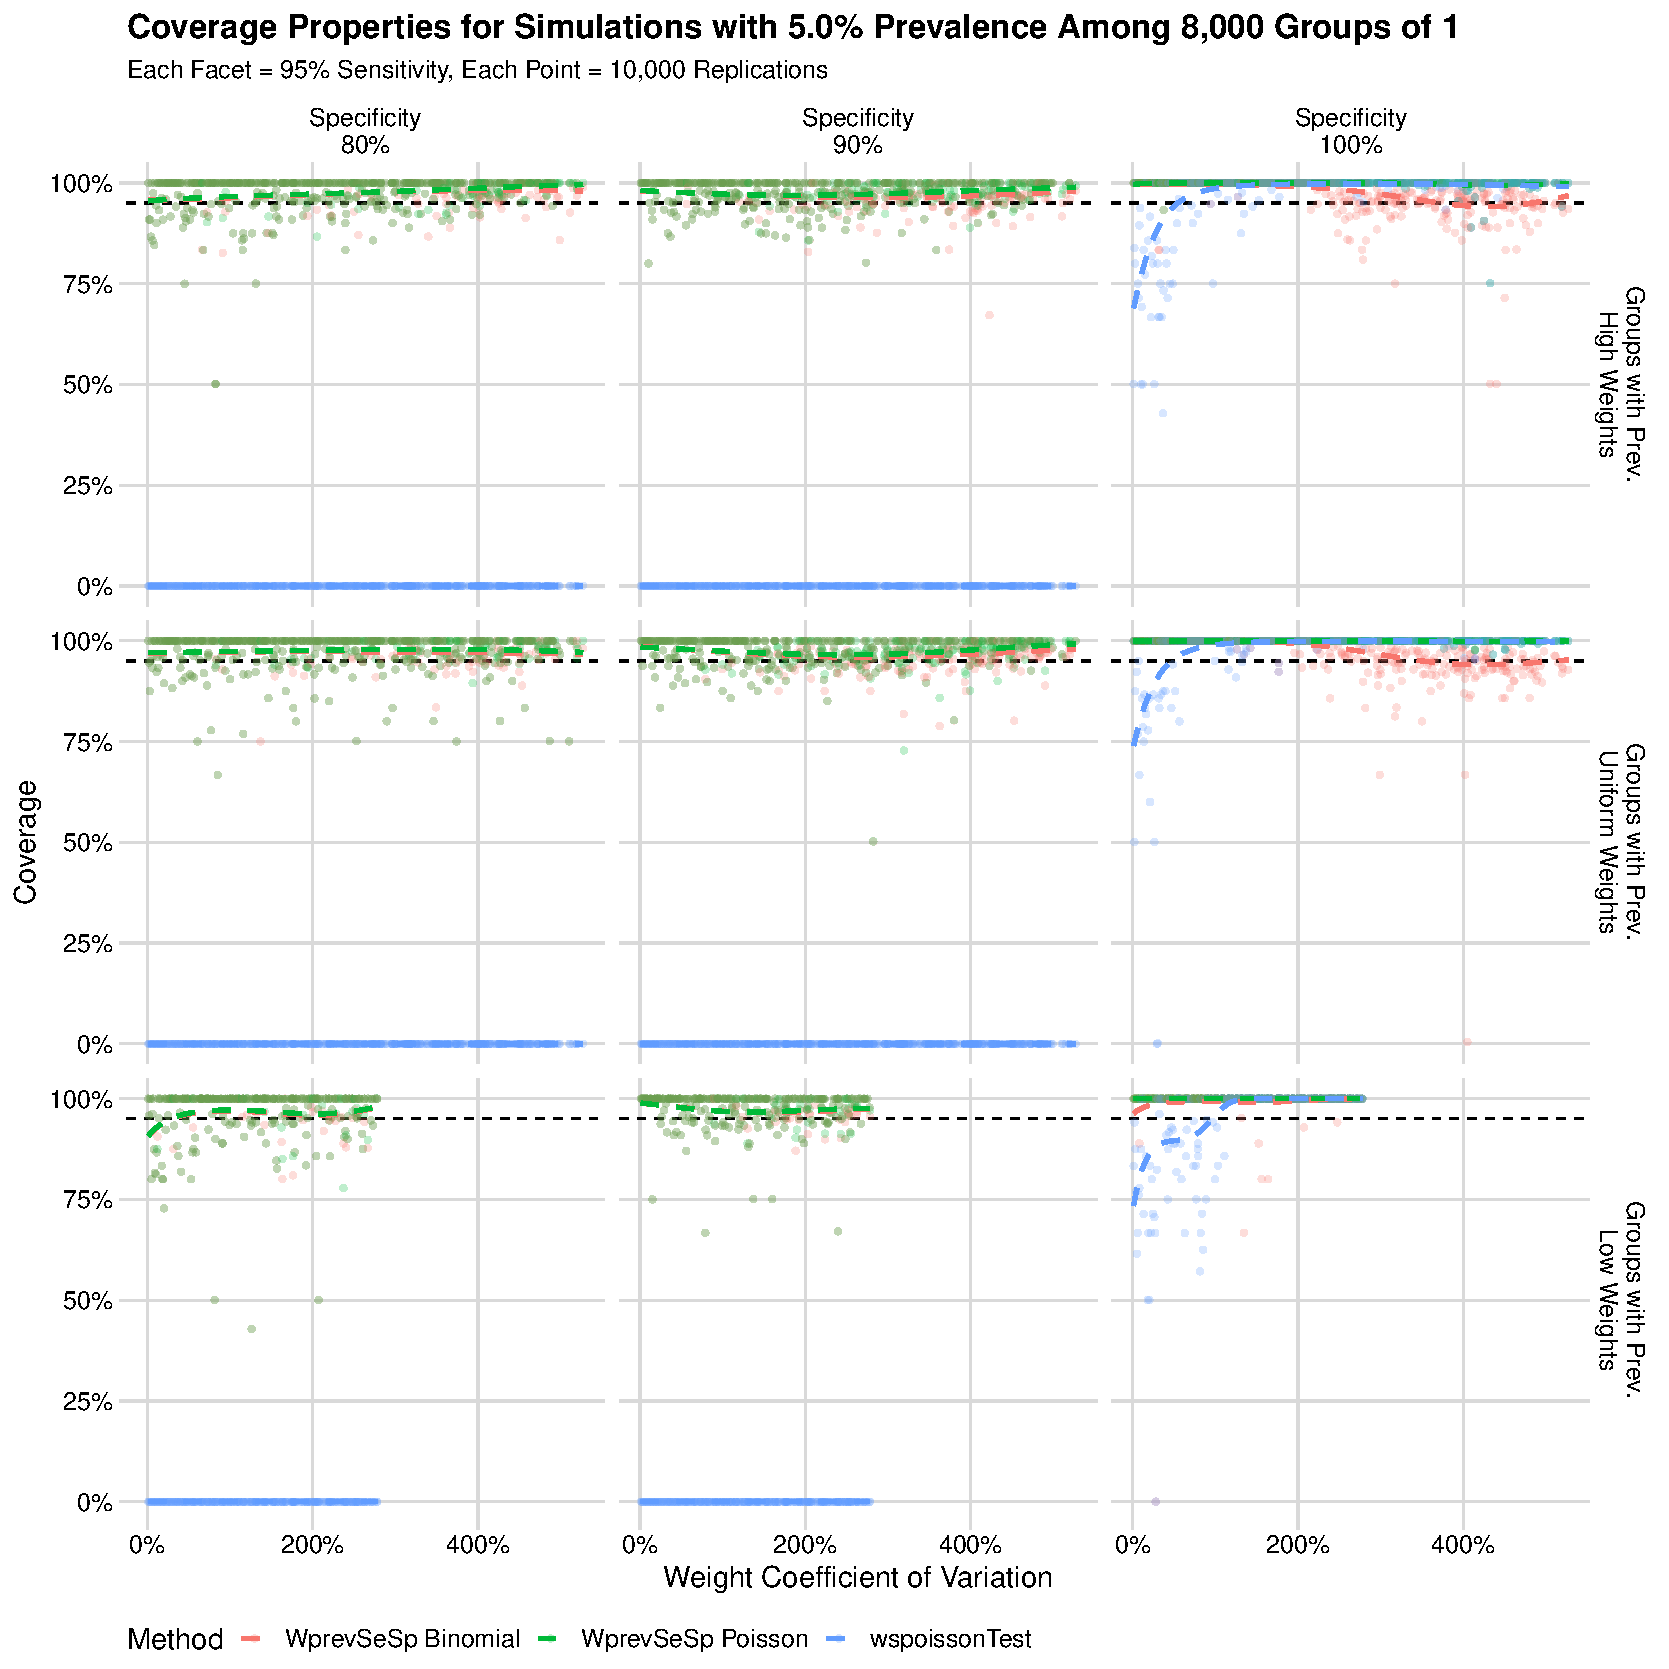
\includegraphics[width=\textwidth]{figures/imperfect_coverage_8000_groups_0_05_prev.pdf}
\caption{Caption}
\label{fig:imperfect_coverage_8000_groups_0_05_prev}
\end{figure}

\begin{figure}
\centering
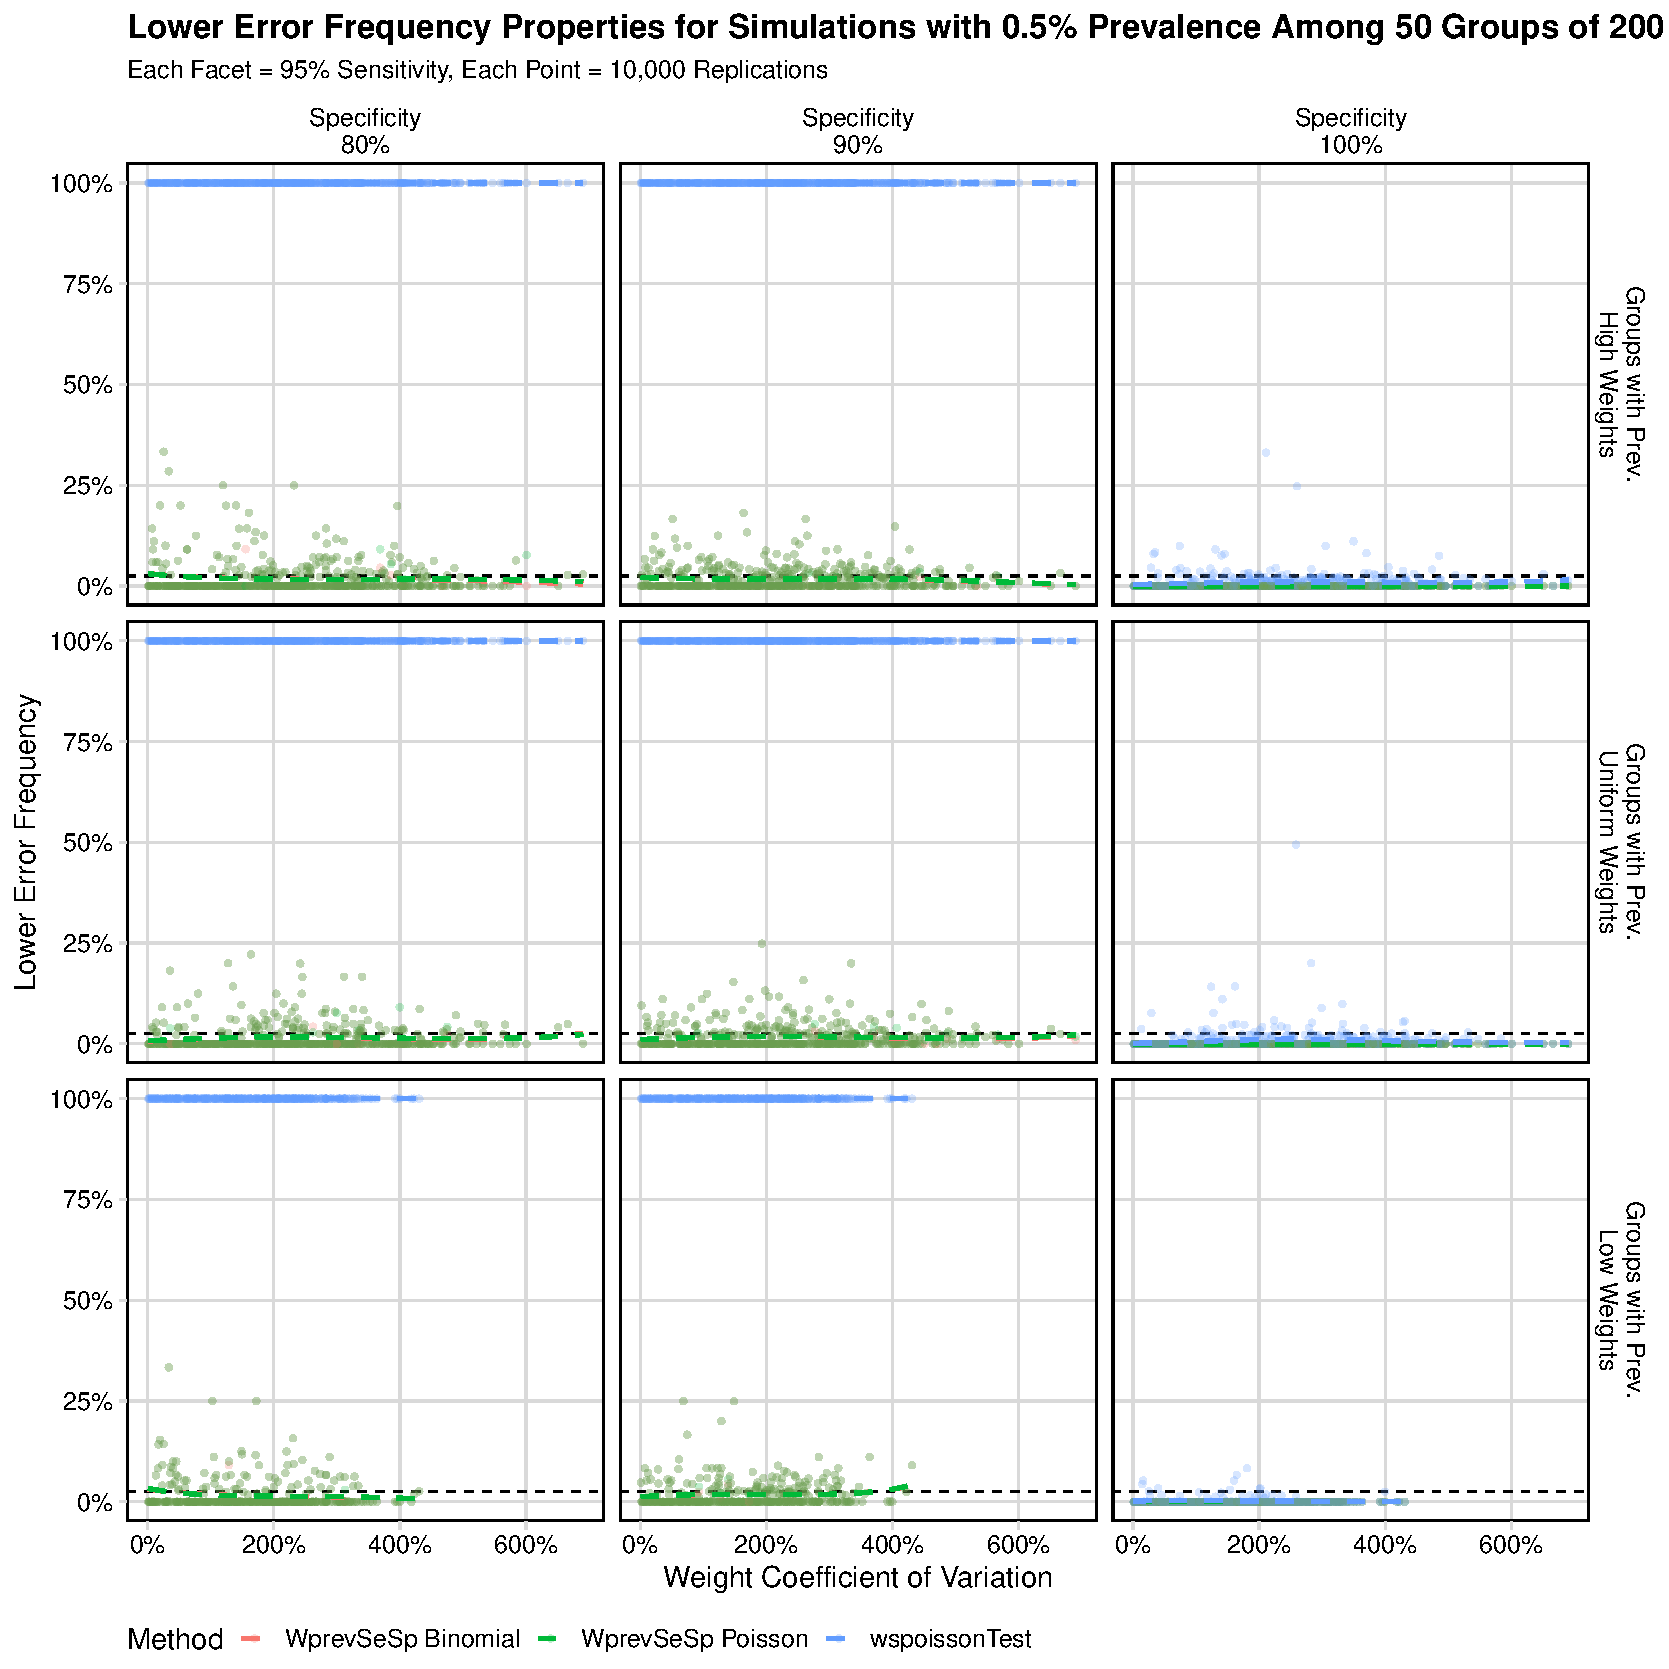
\includegraphics[width=\textwidth]{figures/imperfect_lower_error_frequency_50_groups_0_005_prev.pdf}
\caption{Caption}
\label{fig:imperfect_lower_error_frequency_50_groups_0_005_prev}
\end{figure}

\begin{figure}
\centering
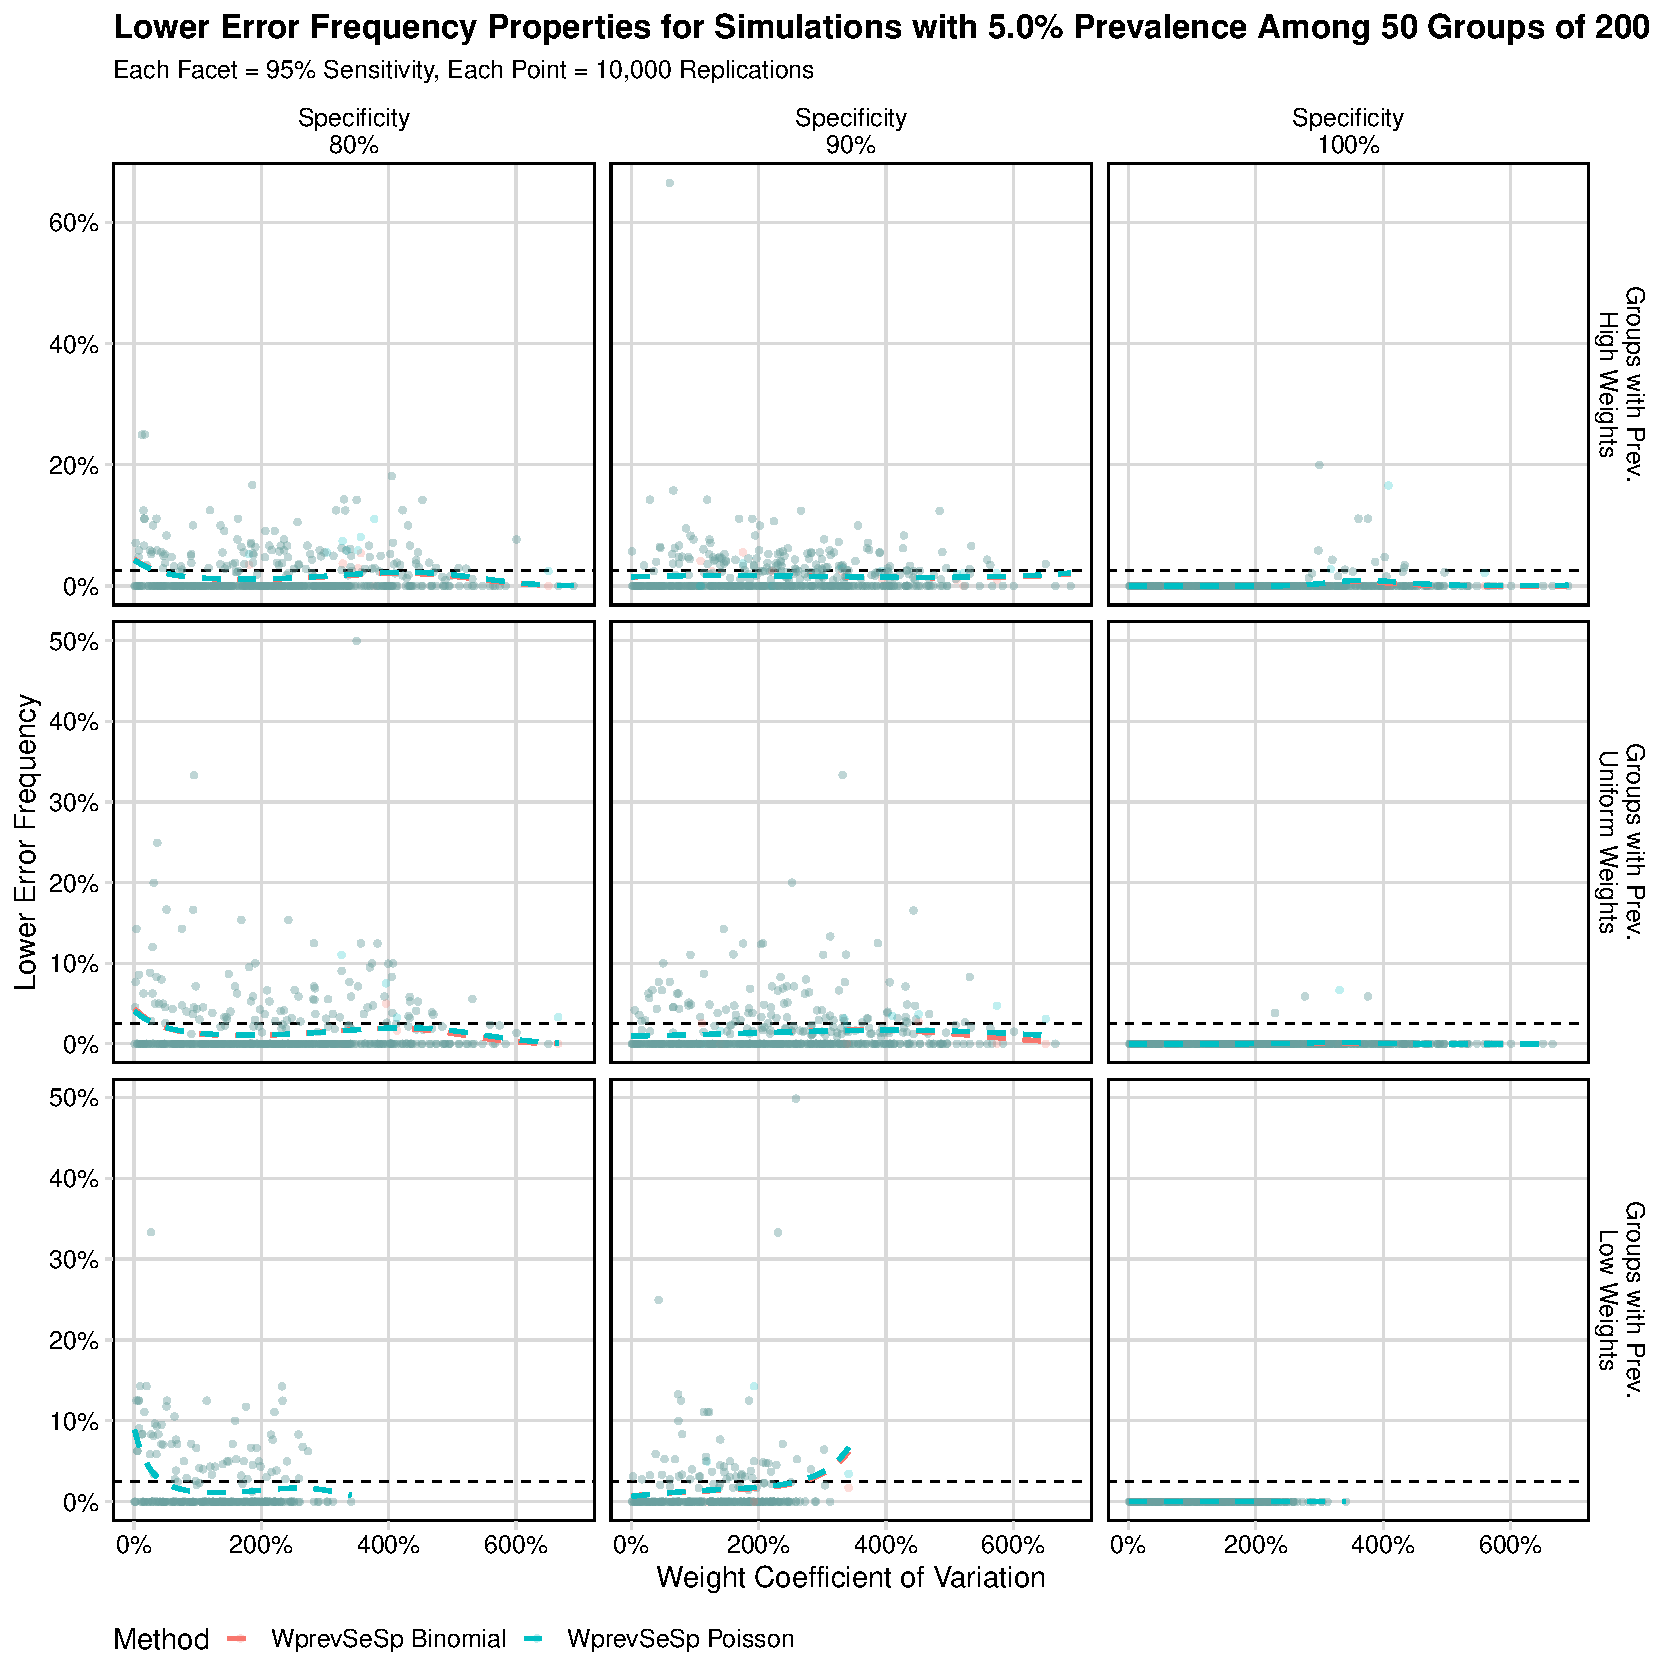
\includegraphics[width=\textwidth]{figures/imperfect_lower_error_frequency_50_groups_0_05_prev.pdf}
\caption{Caption}
\label{fig:imperfect_lower_error_frequency_50_groups_0_05_prev}
\end{figure}

\begin{figure}
\centering
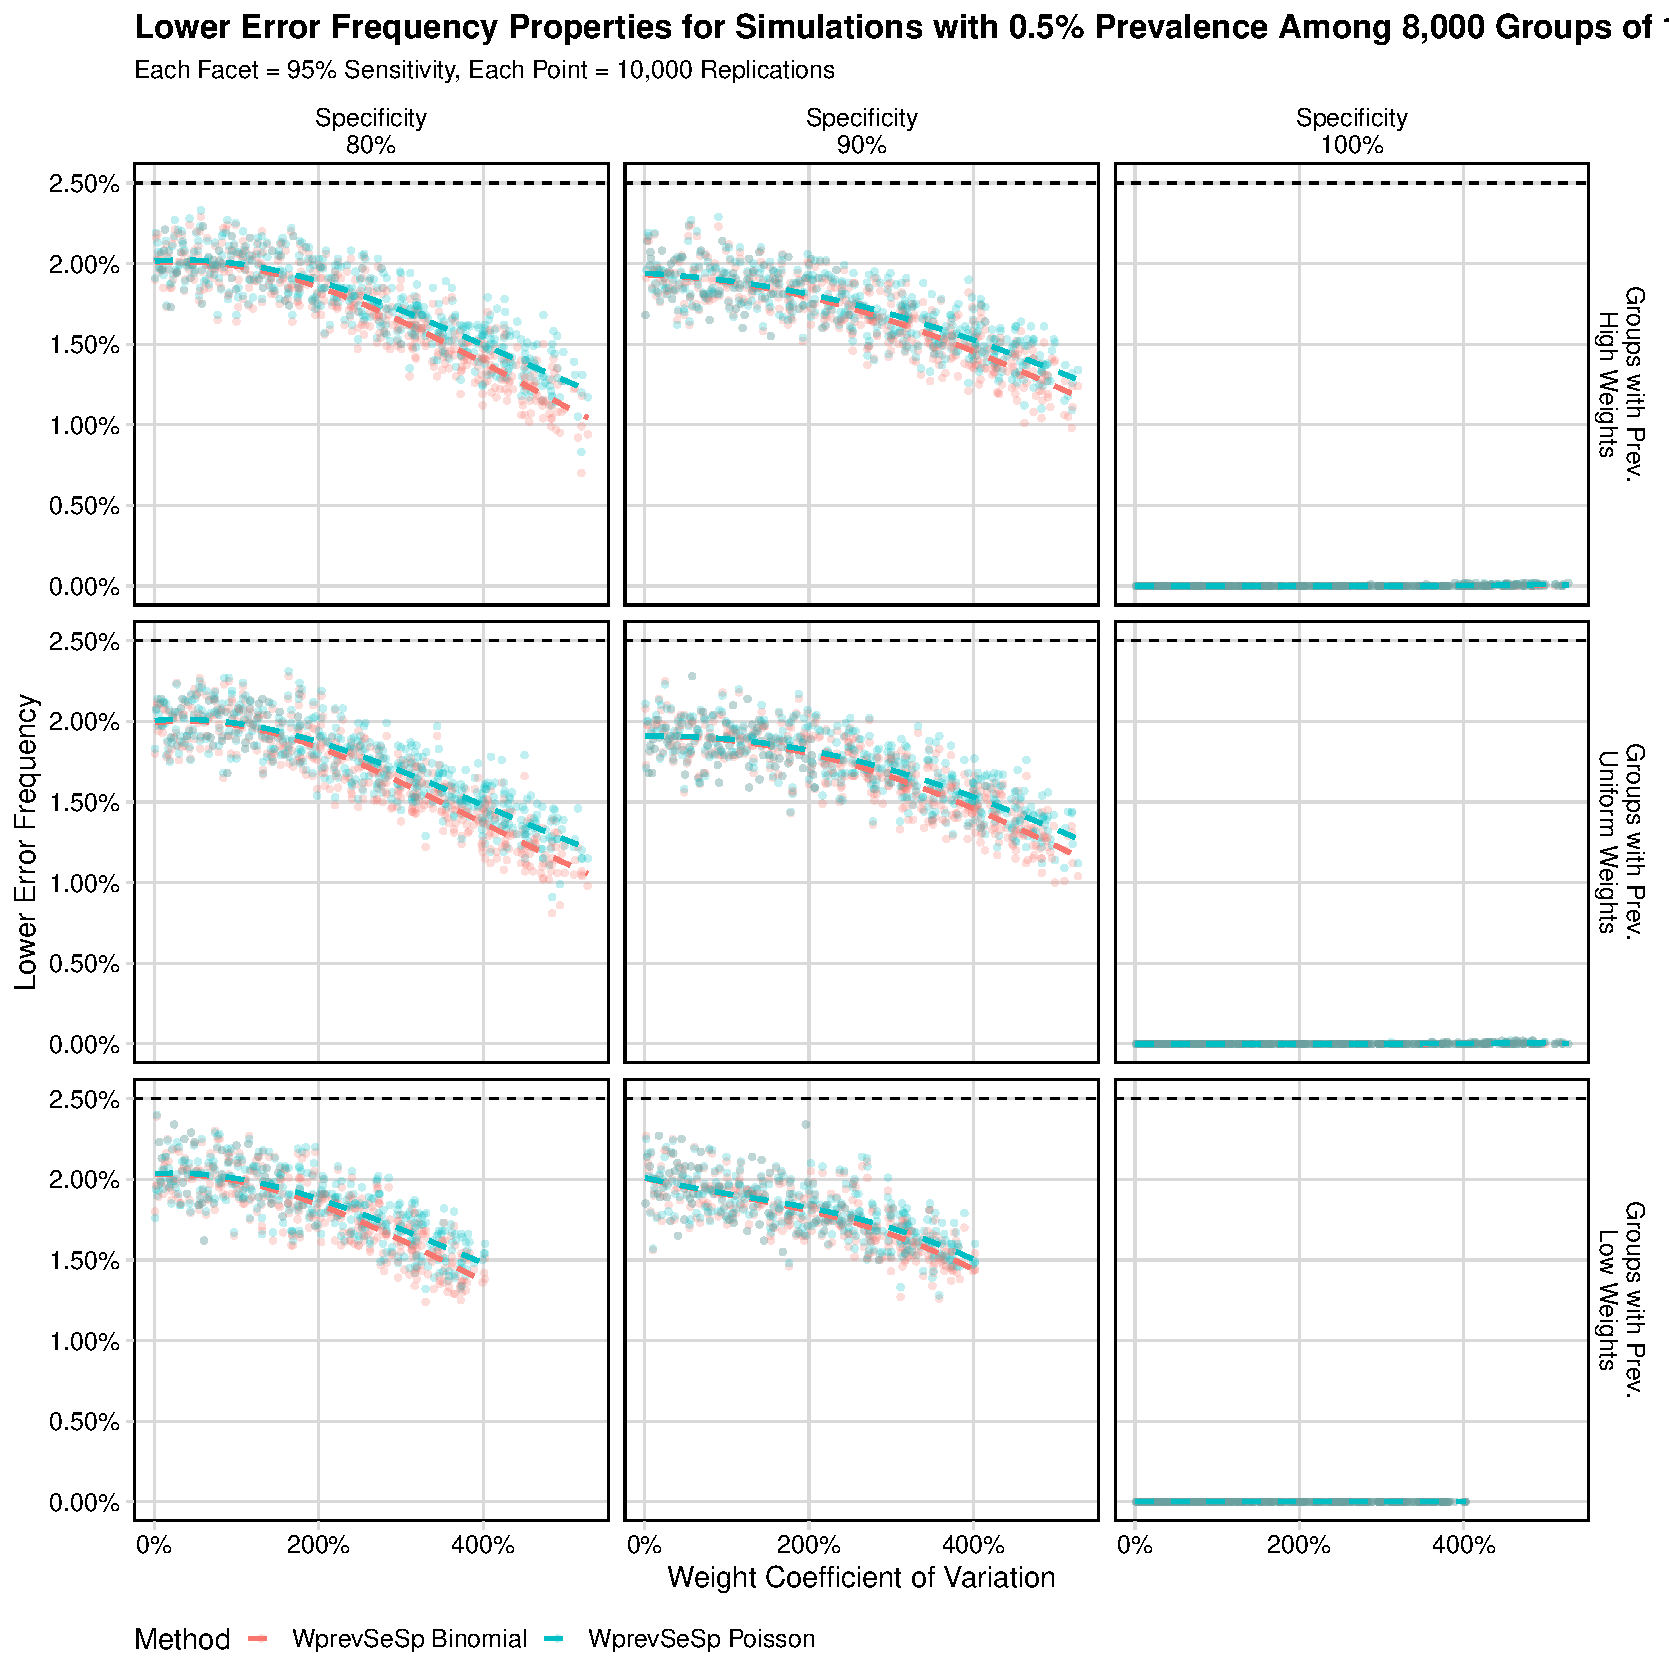
\includegraphics[width=\textwidth]{figures/imperfect_lower_error_frequency_8000_groups_0_005_prev.pdf}
\caption{Caption}
\label{fig:imperfect_lower_error_frequency_8000_groups_0_005_prev}
\end{figure}

\begin{figure}
\centering
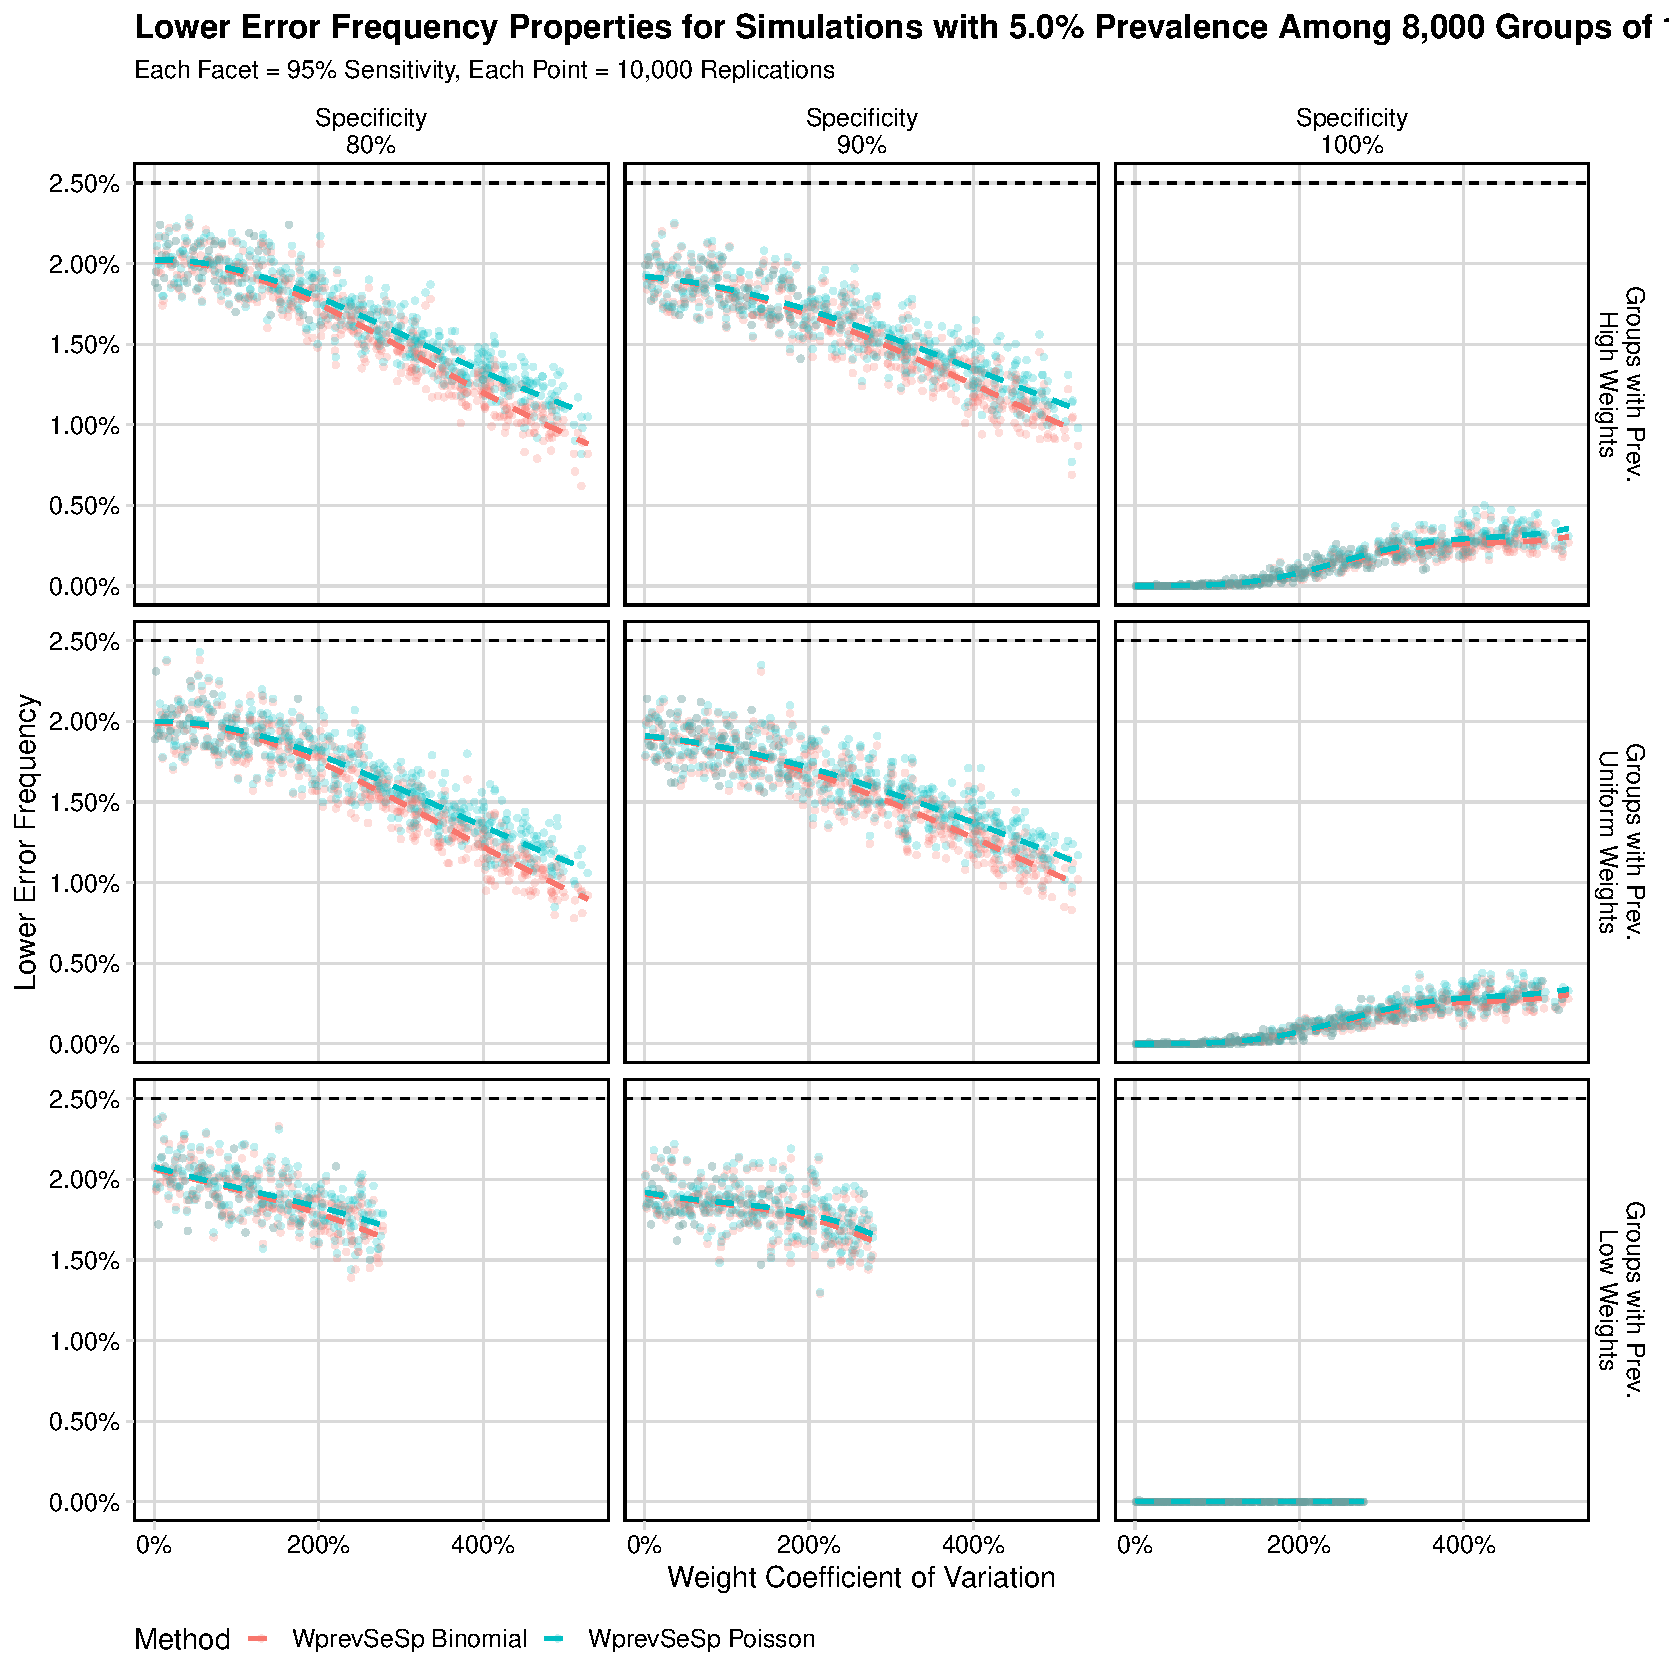
\includegraphics[width=\textwidth]{figures/imperfect_lower_error_frequency_8000_groups_0_05_prev.pdf}
\caption{Caption}
\label{fig:imperfect_lower_error_frequency_8000_groups_0_05_prev}
\end{figure}

\begin{figure}
\centering
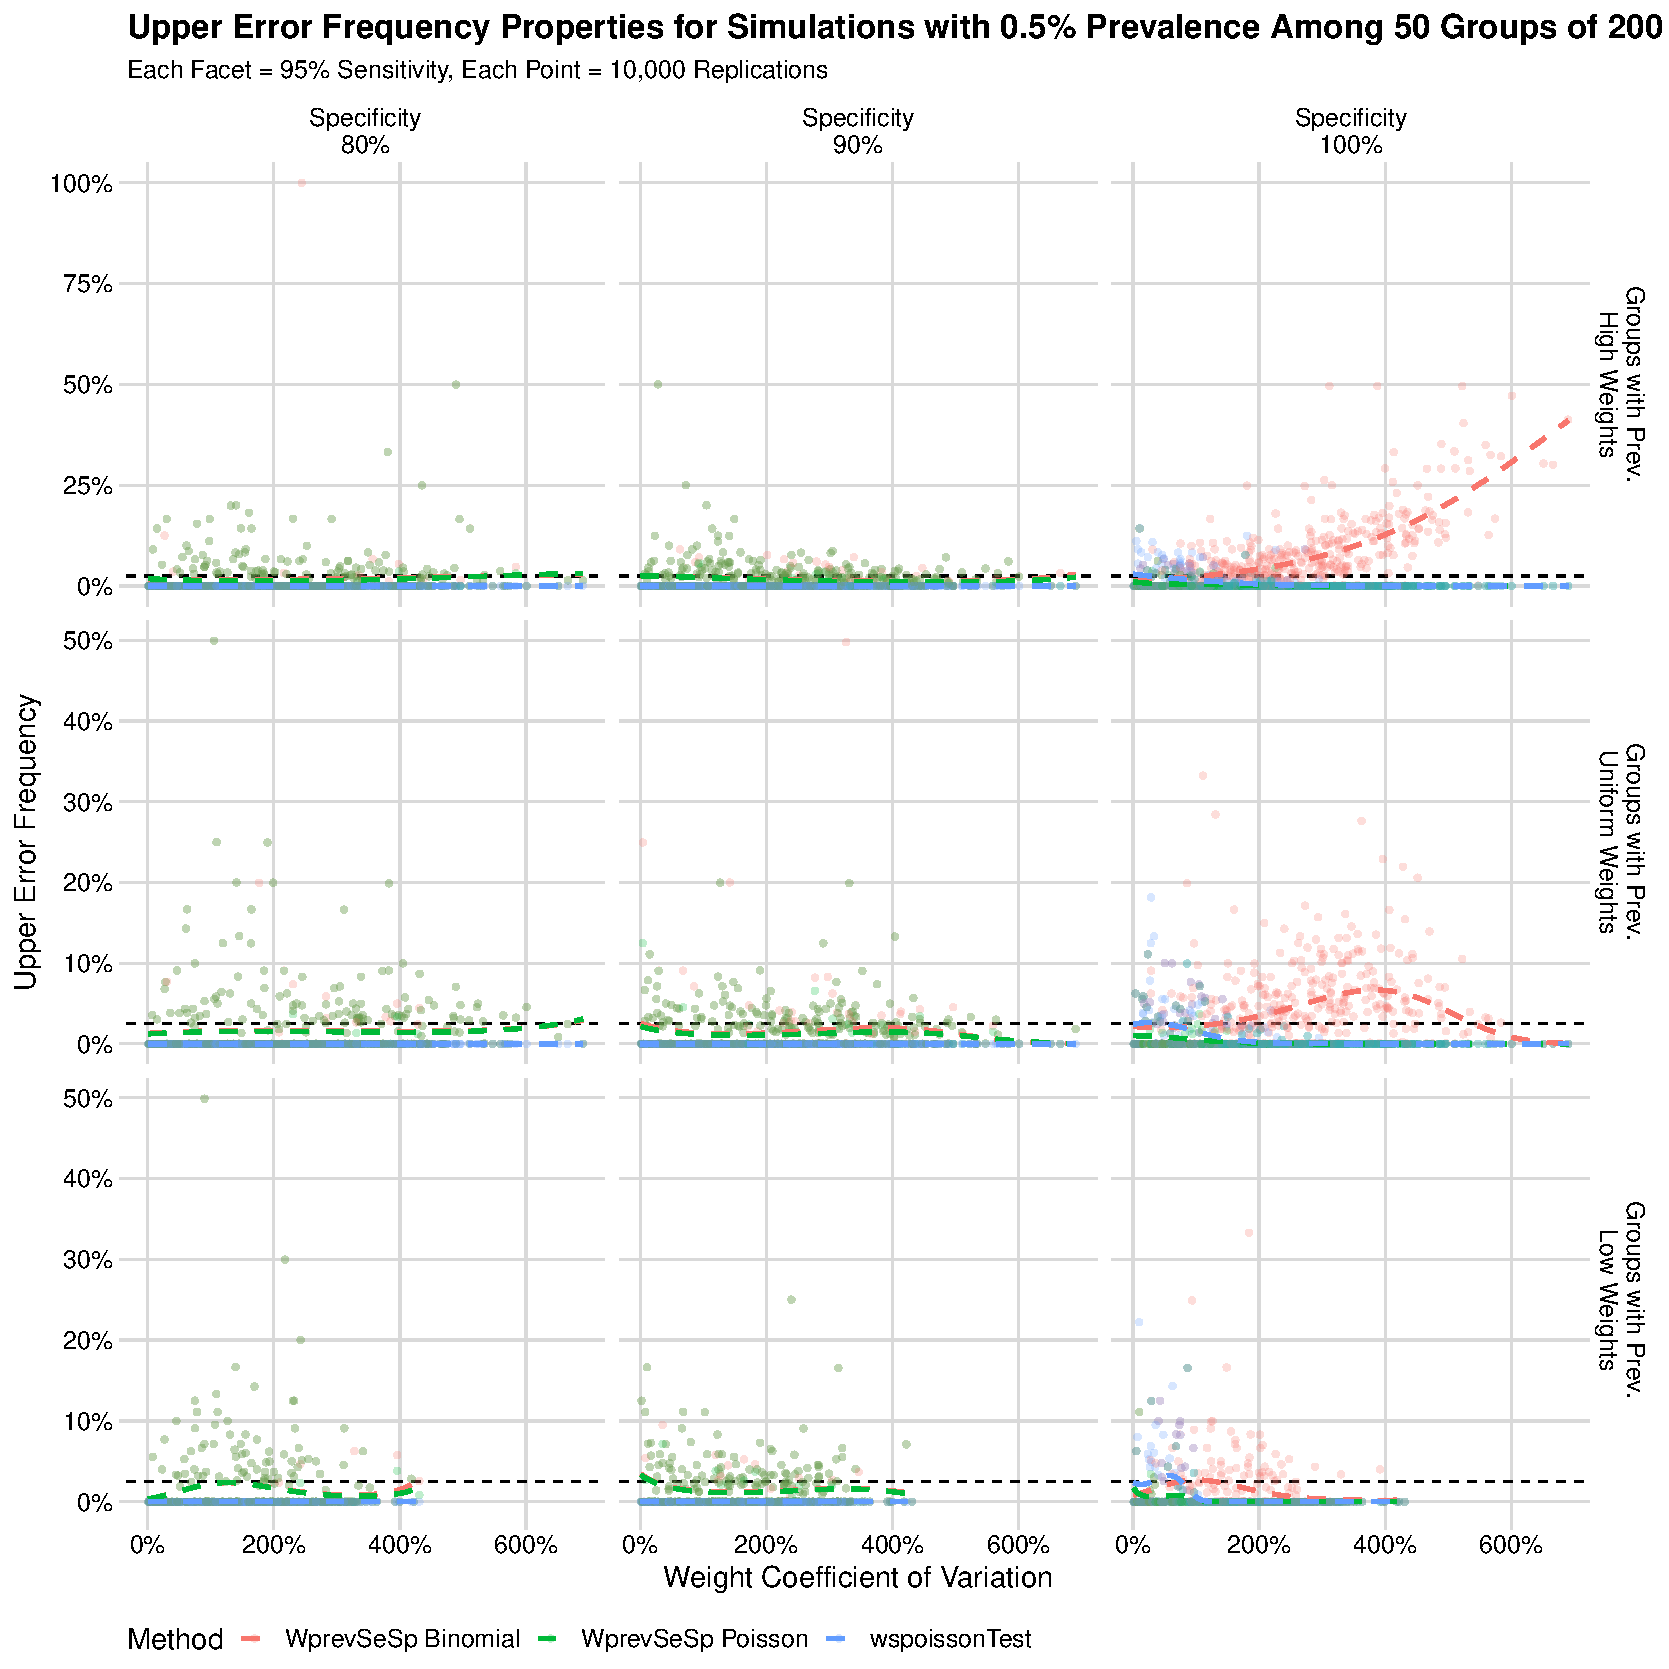
\includegraphics[width=\textwidth]{figures/imperfect_upper_error_frequency_50_groups_0_005_prev.pdf}
\caption{Caption}
\label{fig:imperfect_upper_error_frequency_50_groups_0_005_prev}
\end{figure}

\begin{figure}
\centering
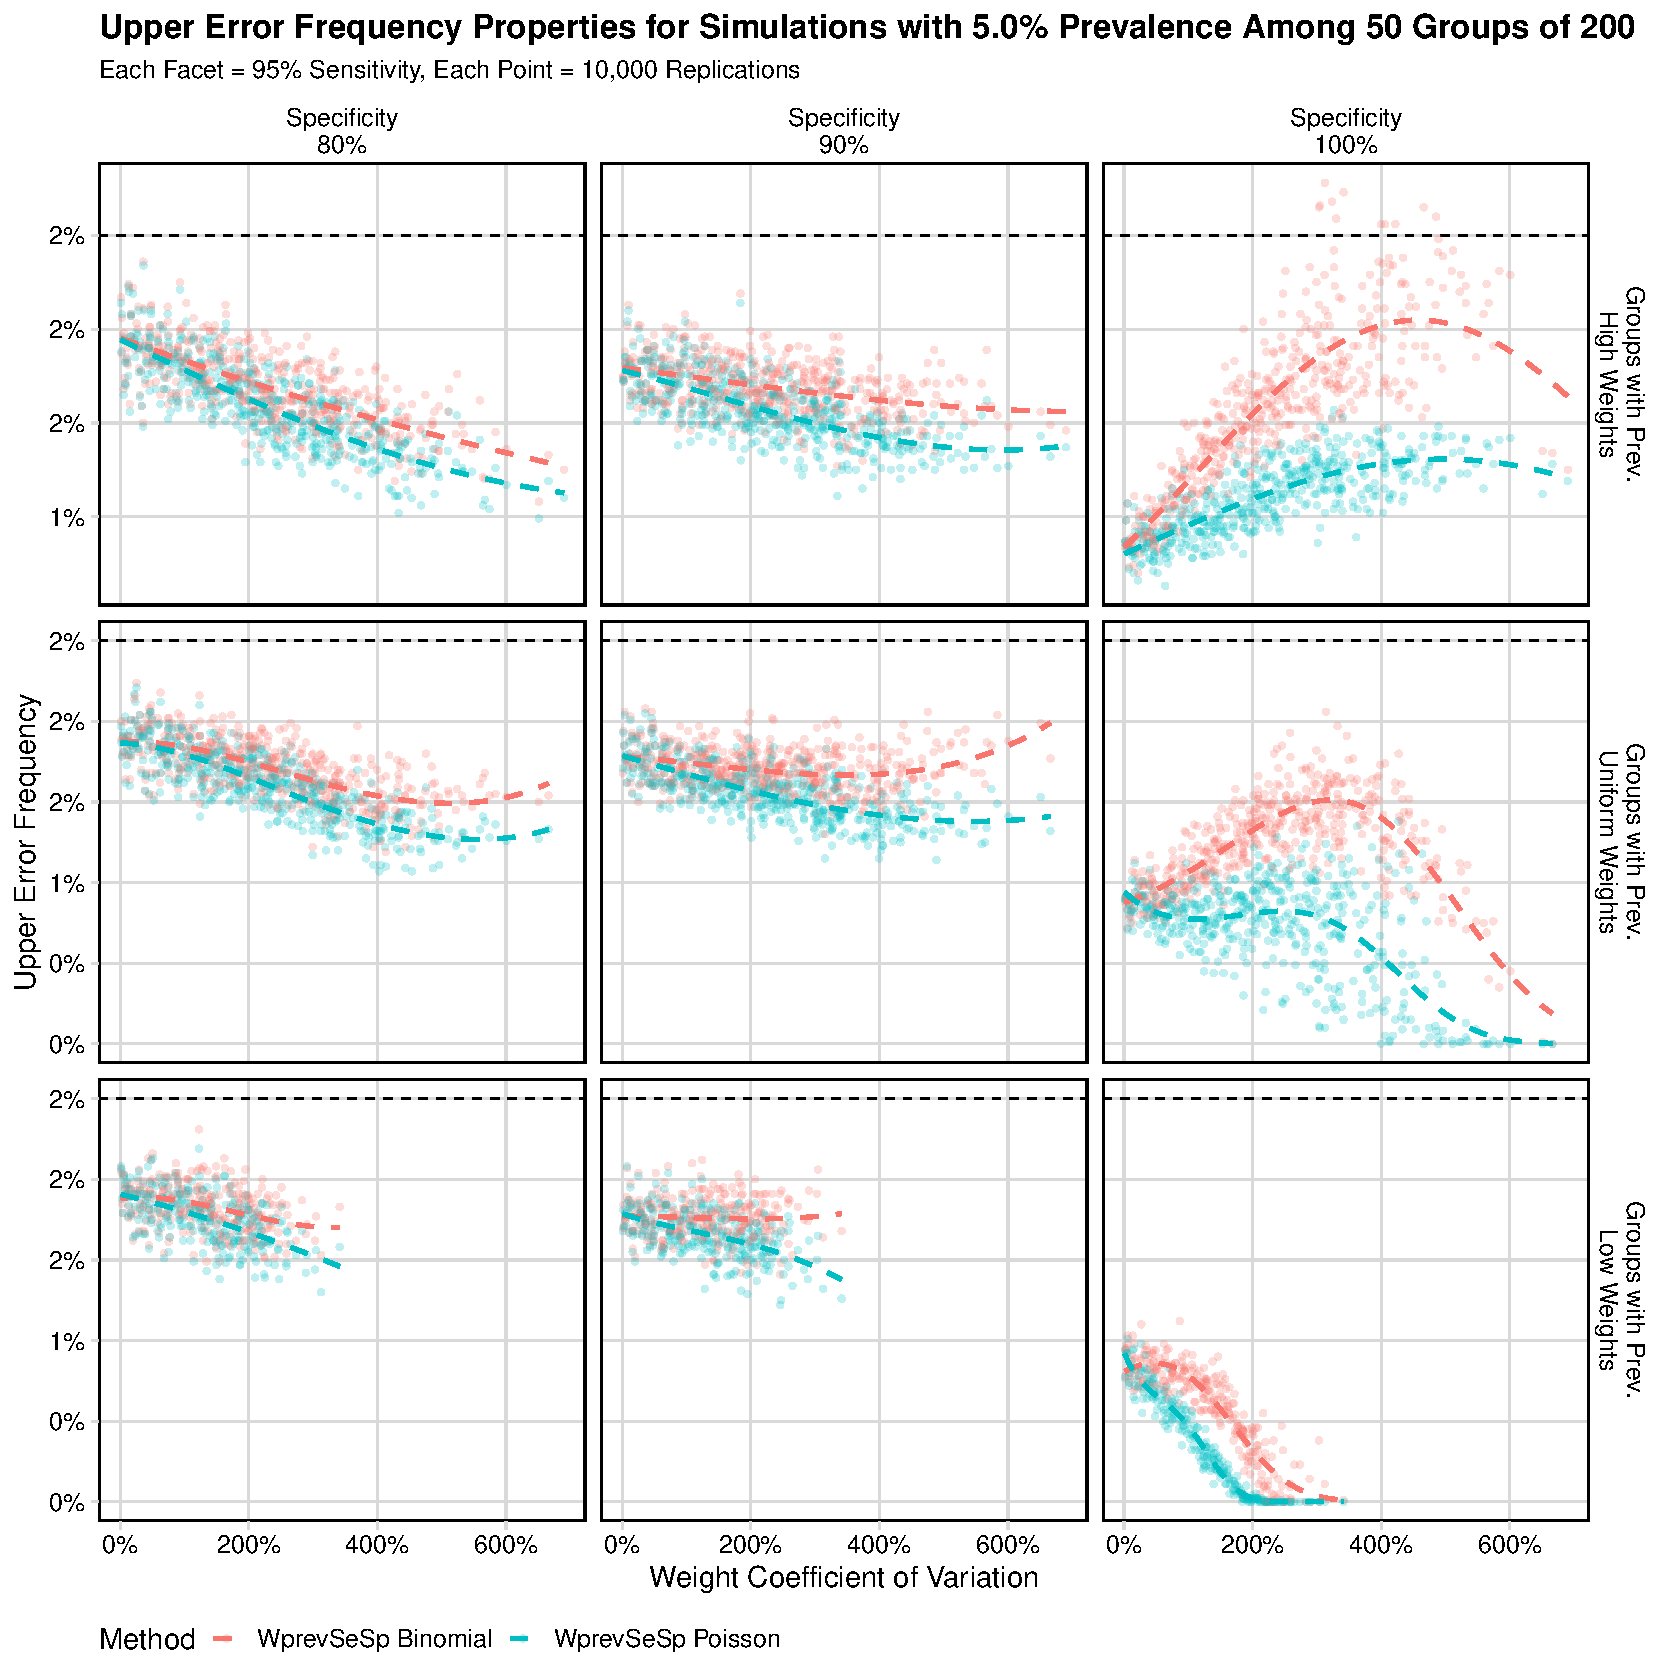
\includegraphics[width=\textwidth]{figures/imperfect_upper_error_frequency_50_groups_0_05_prev.pdf}
\caption{Caption}
\label{fig:imperfect_upper_error_frequency_50_groups_0_05_prev}
\end{figure}

\begin{figure}
\centering
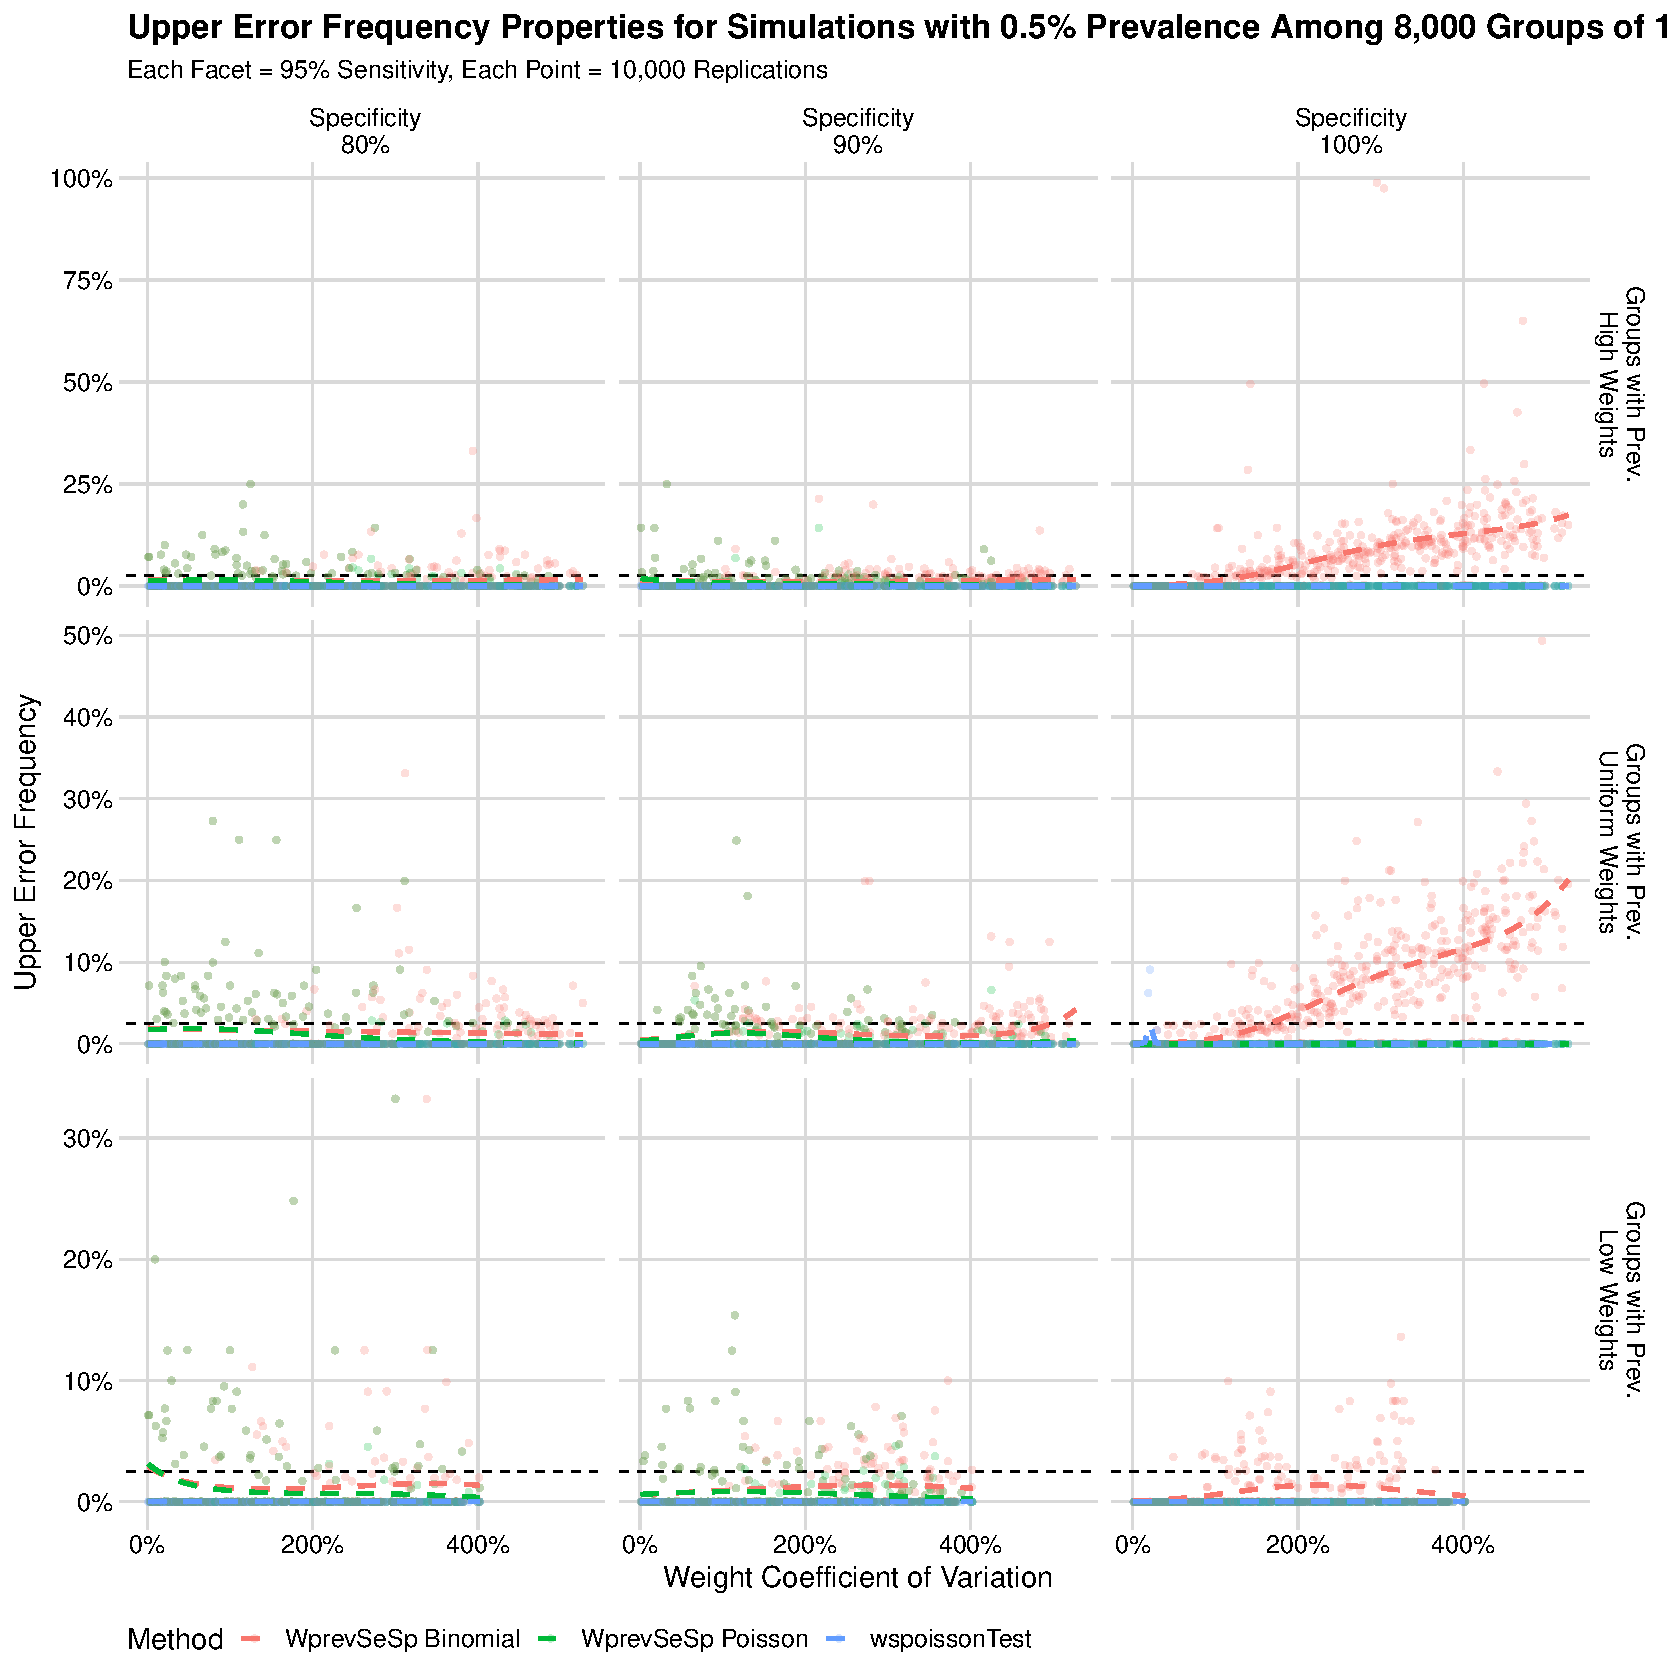
\includegraphics[width=\textwidth]{figures/imperfect_upper_error_frequency_8000_groups_0_005_prev.pdf}
\caption{Caption}
\label{fig:imperfect_upper_error_frequency_8000_groups_0_005_prev}
\end{figure}

\begin{figure}
\centering
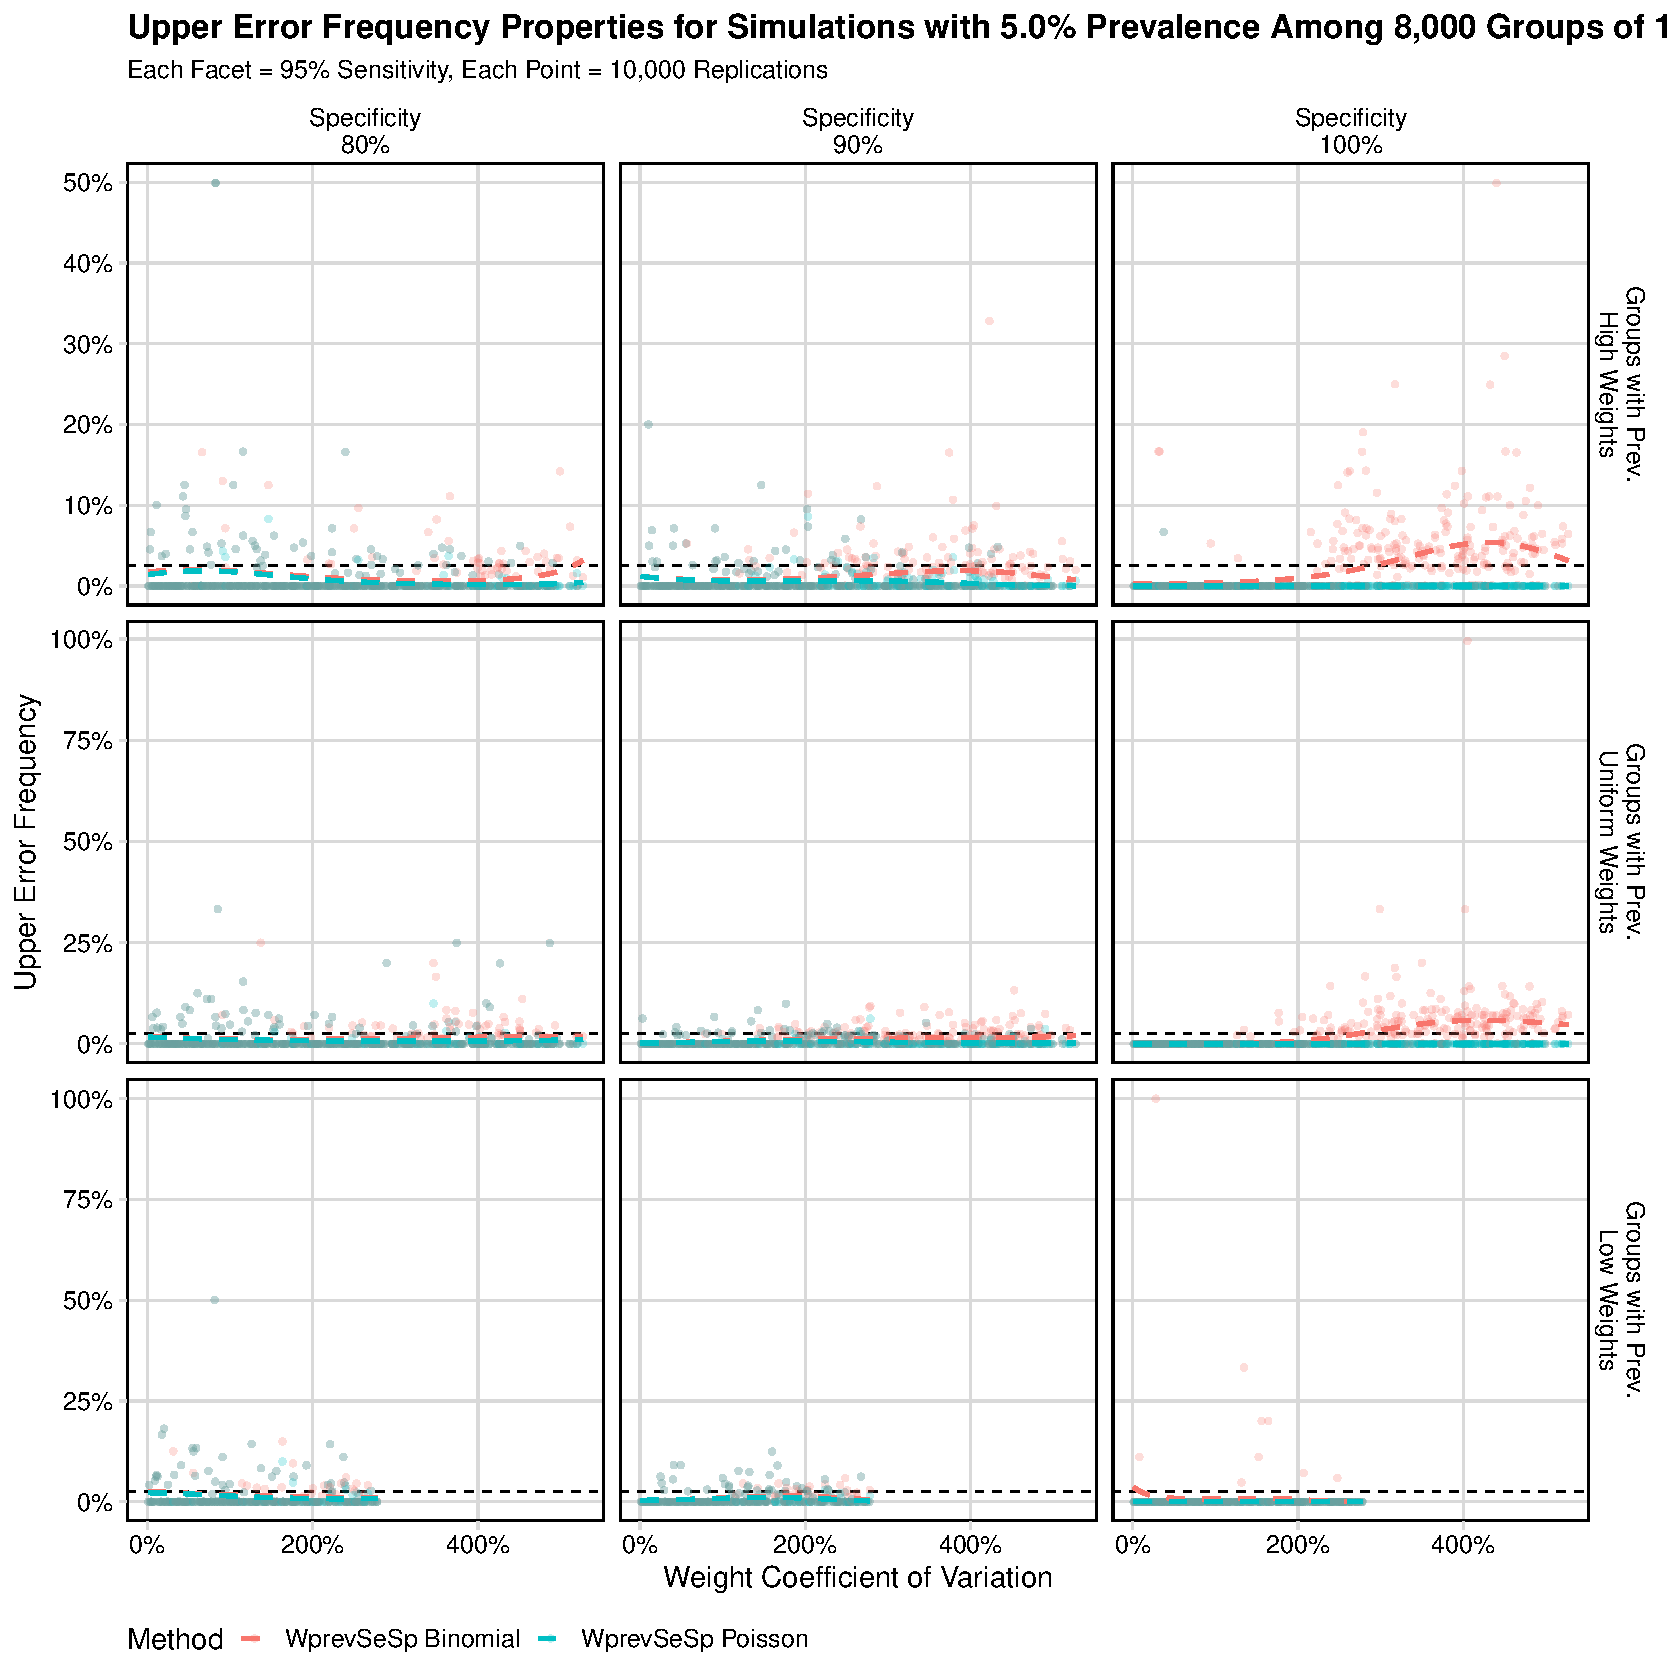
\includegraphics[width=\textwidth]{figures/imperfect_upper_error_frequency_8000_groups_0_05_prev.pdf}
\caption{Caption}
\label{fig:imperfect_upper_error_frequency_8000_groups_0_05_prev}
\end{figure}

\begin{figure}
\centering
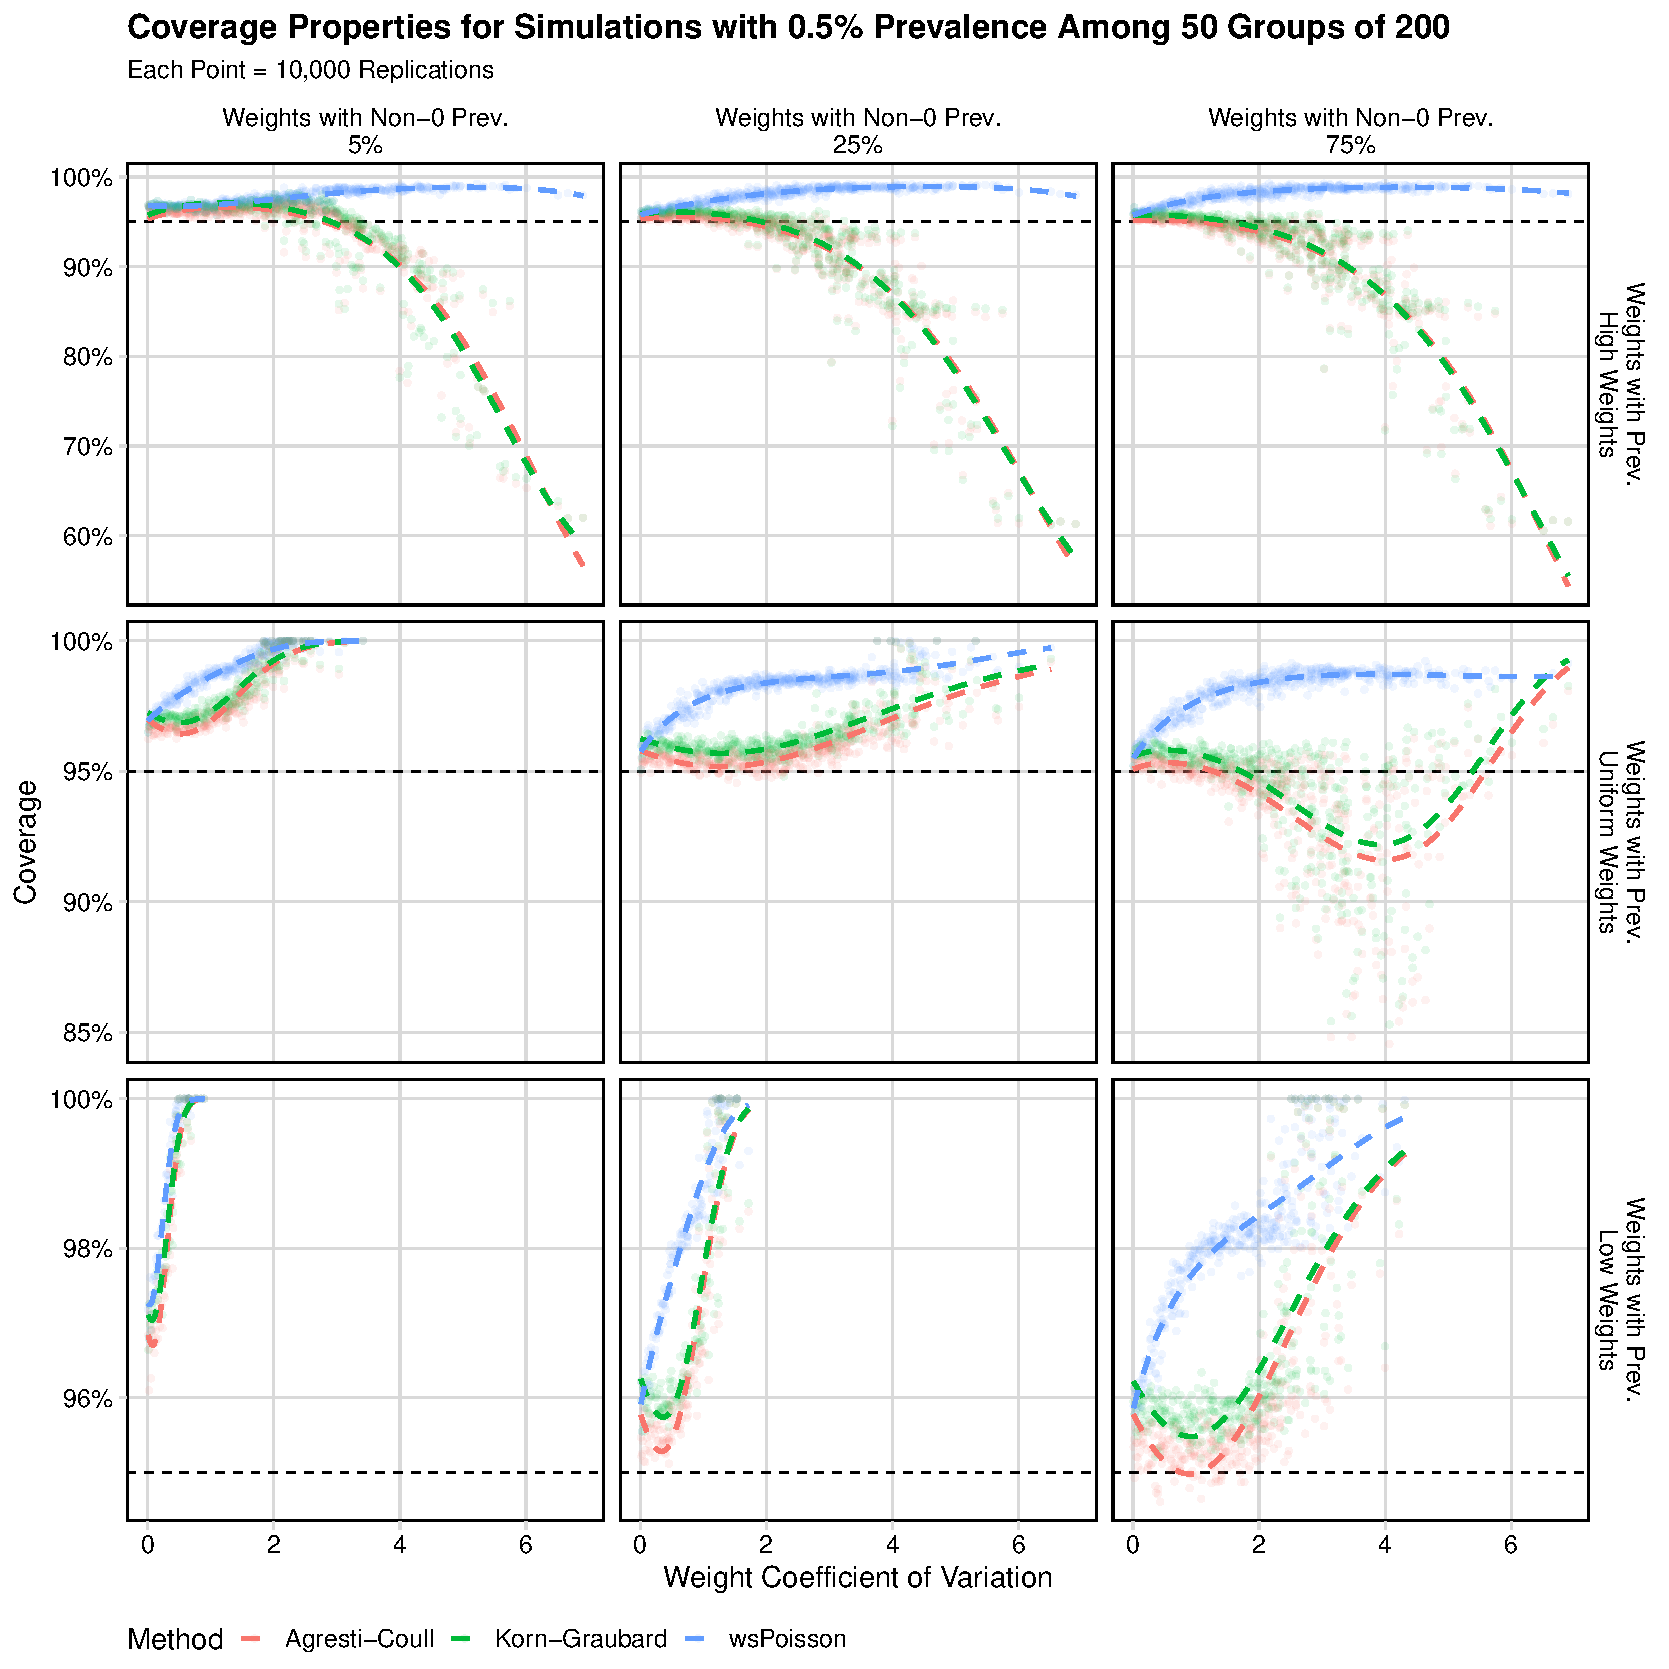
\includegraphics[width=\textwidth]{figures/perfect_coverage_50_groups_0_005_prev.pdf}
\caption{Caption}
\label{fig:perfect_coverage_50_groups_0_005_prev}
\end{figure}

\begin{figure}
\centering
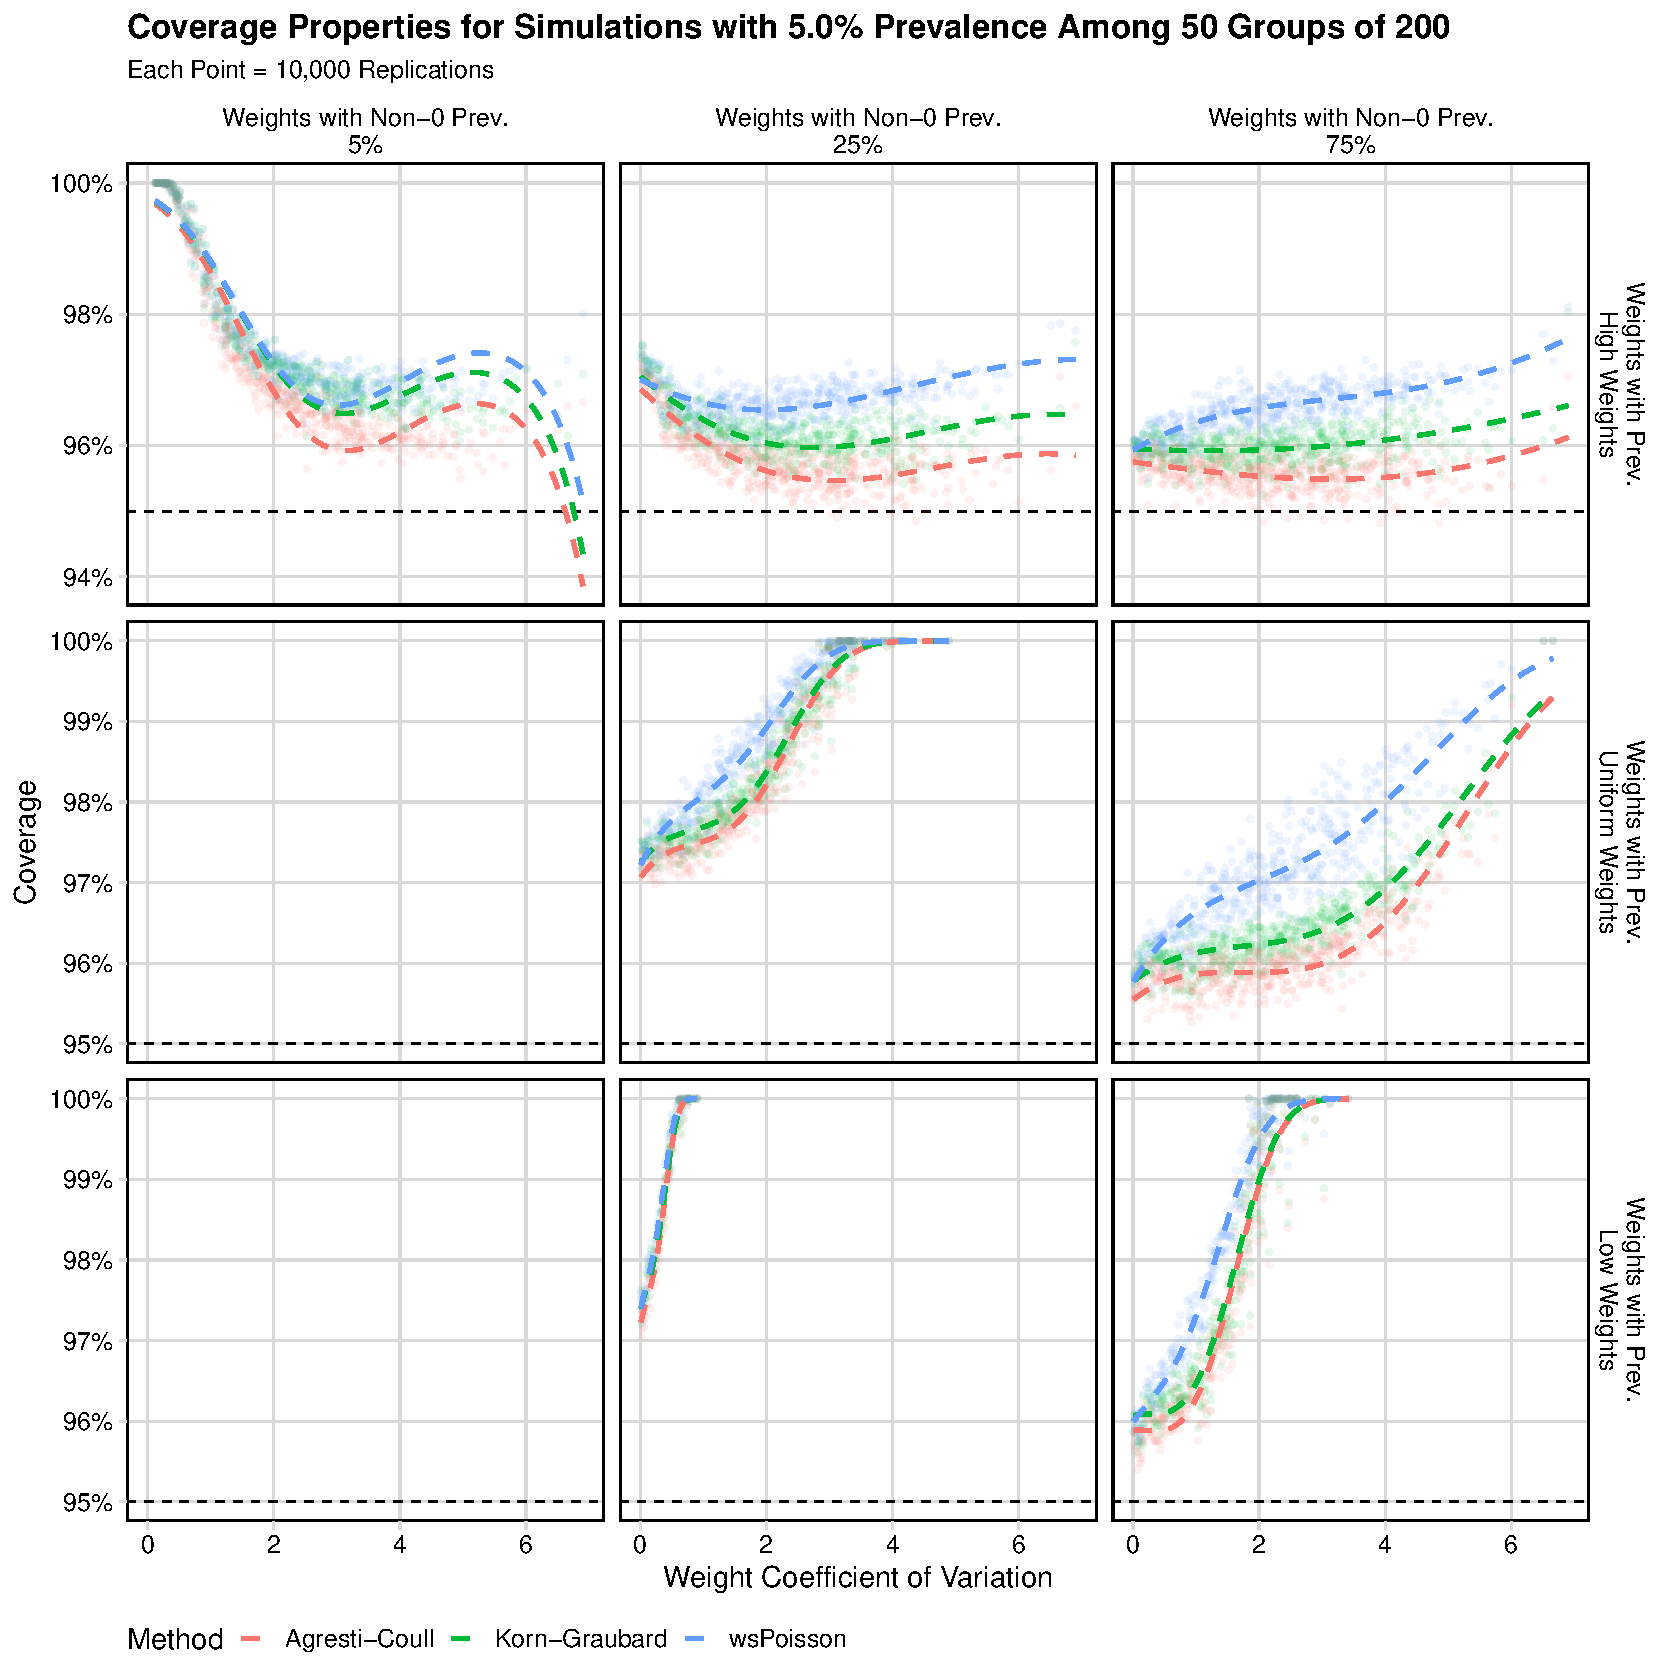
\includegraphics[width=\textwidth]{figures/perfect_coverage_50_groups_0_05_prev.pdf}
\caption{Caption}
\label{fig:perfect_coverage_50_groups_0_05_prev}
\end{figure}

\begin{figure}
\centering
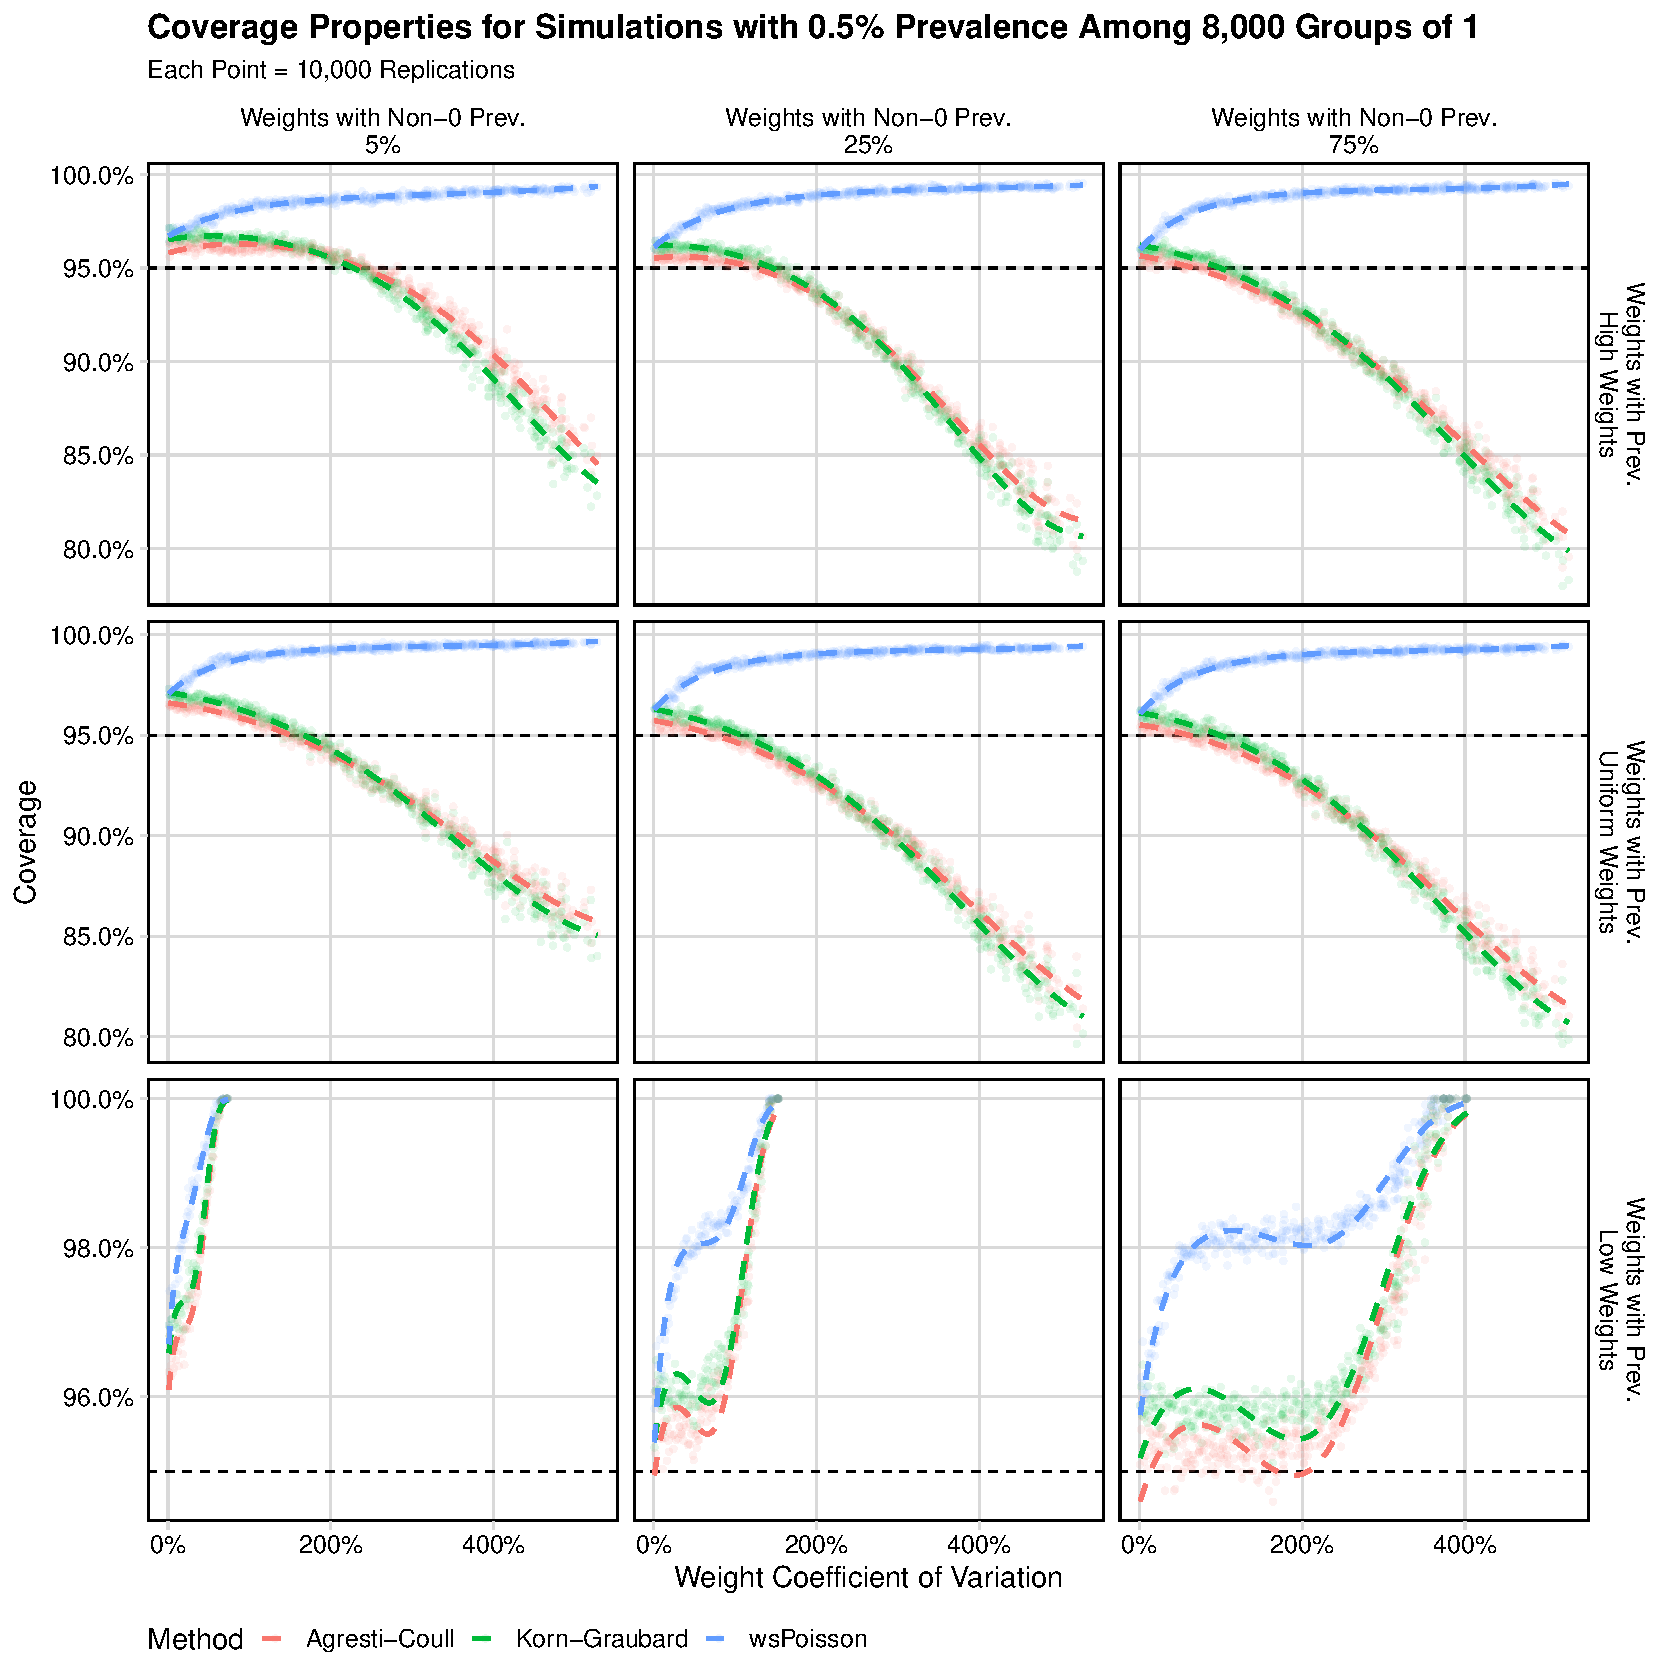
\includegraphics[width=\textwidth]{figures/perfect_coverage_8000_groups_0_005_prev.pdf}
\caption{Caption}
\label{fig:perfect_coverage_8000_groups_0_005_prev}
\end{figure}

\begin{figure}
\centering
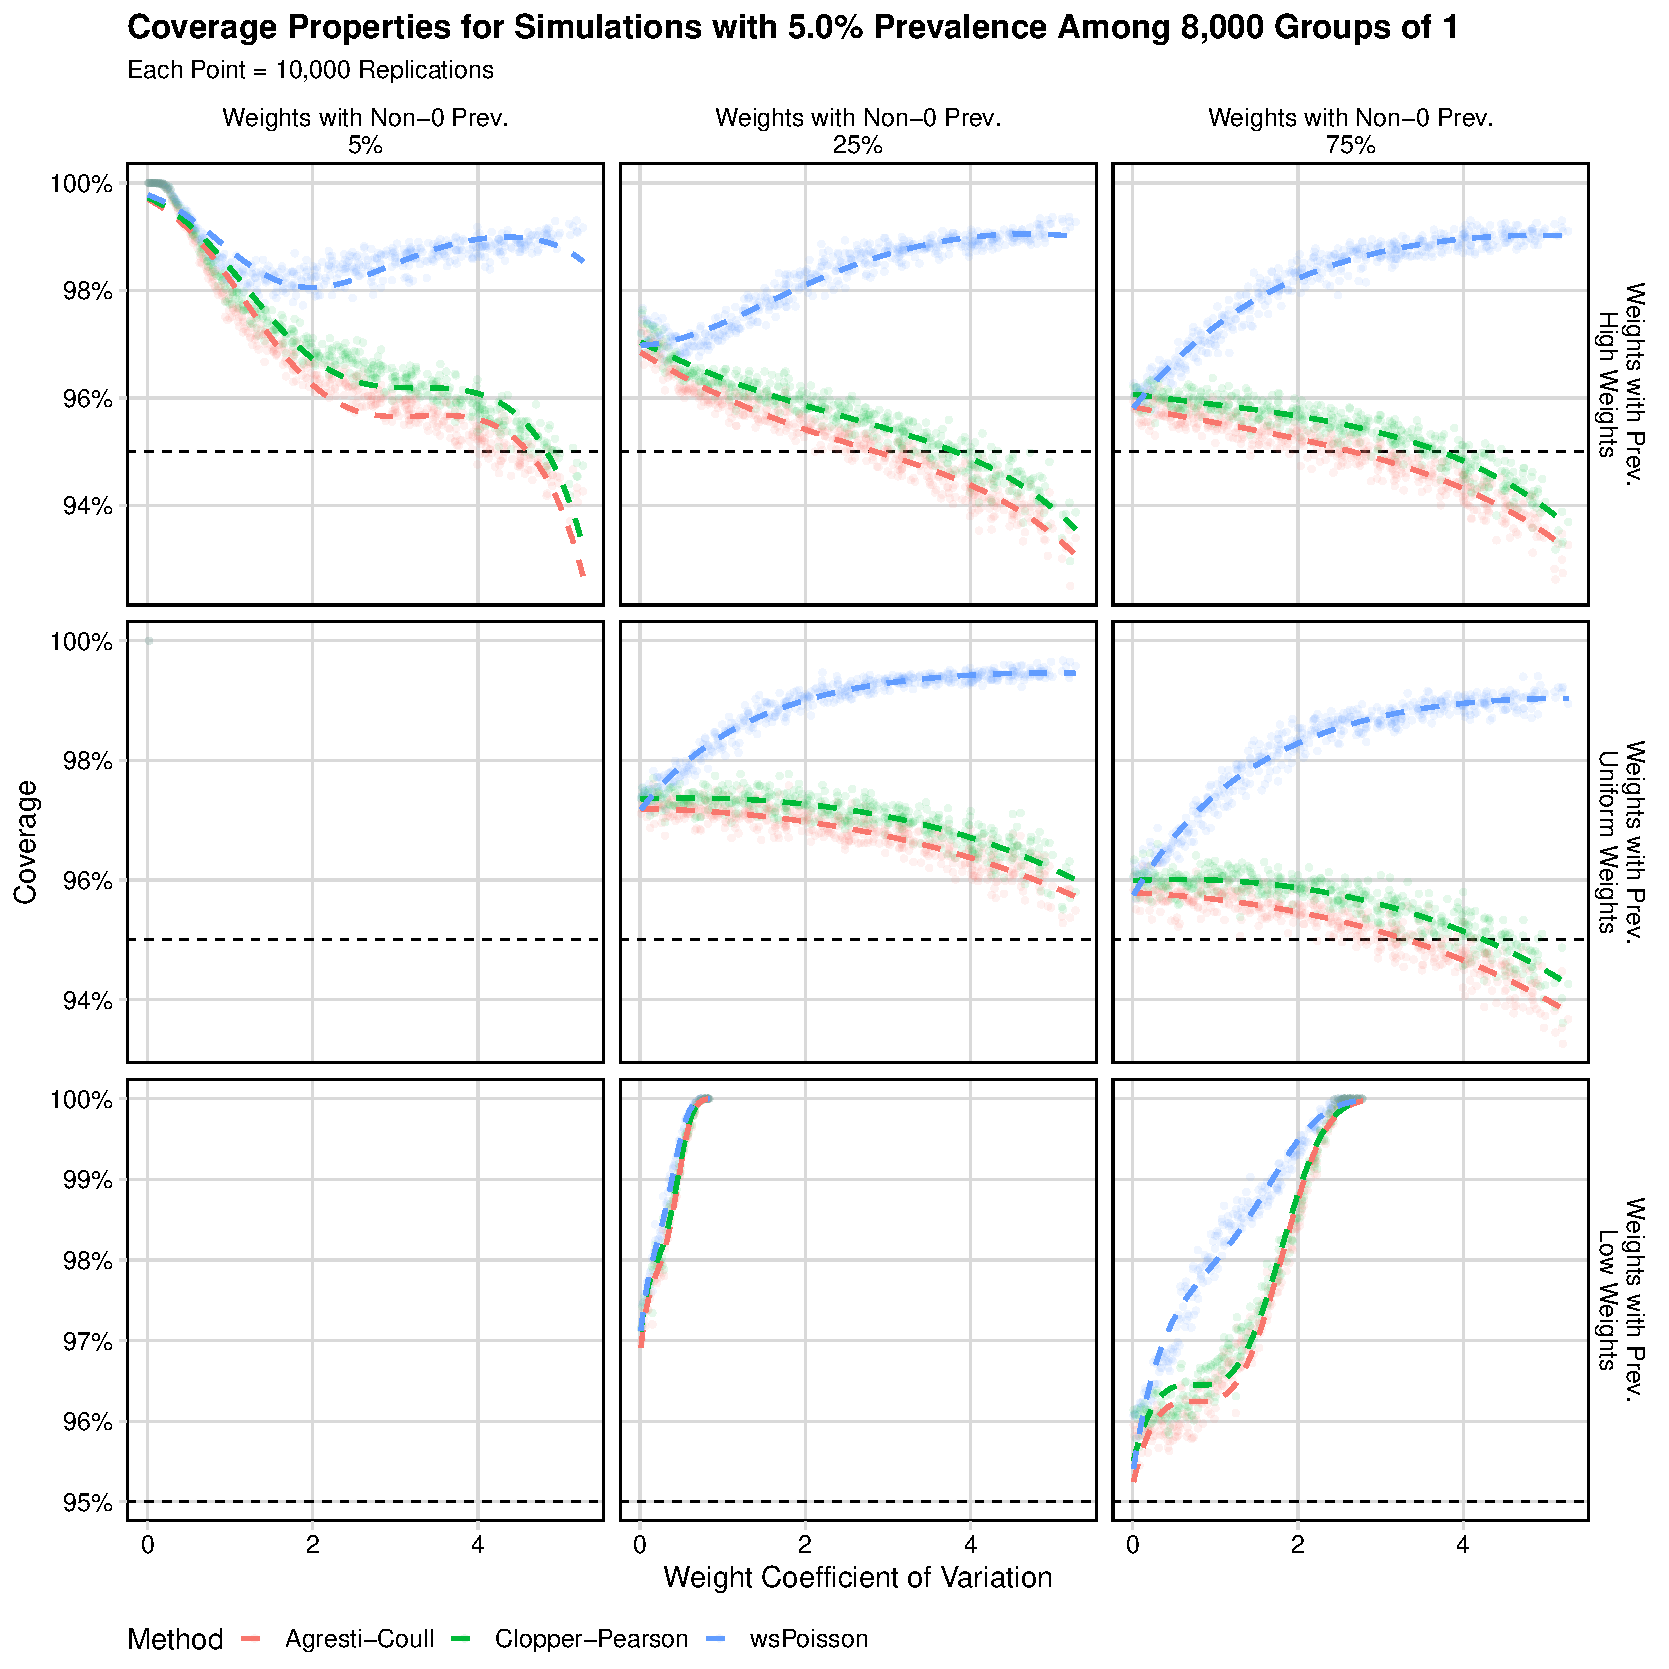
\includegraphics[width=\textwidth]{figures/perfect_coverage_8000_groups_0_05_prev.pdf}
\caption{Caption}
\label{fig:perfect_coverage_8000_groups_0_05_prev}
\end{figure}

\begin{figure}
\centering
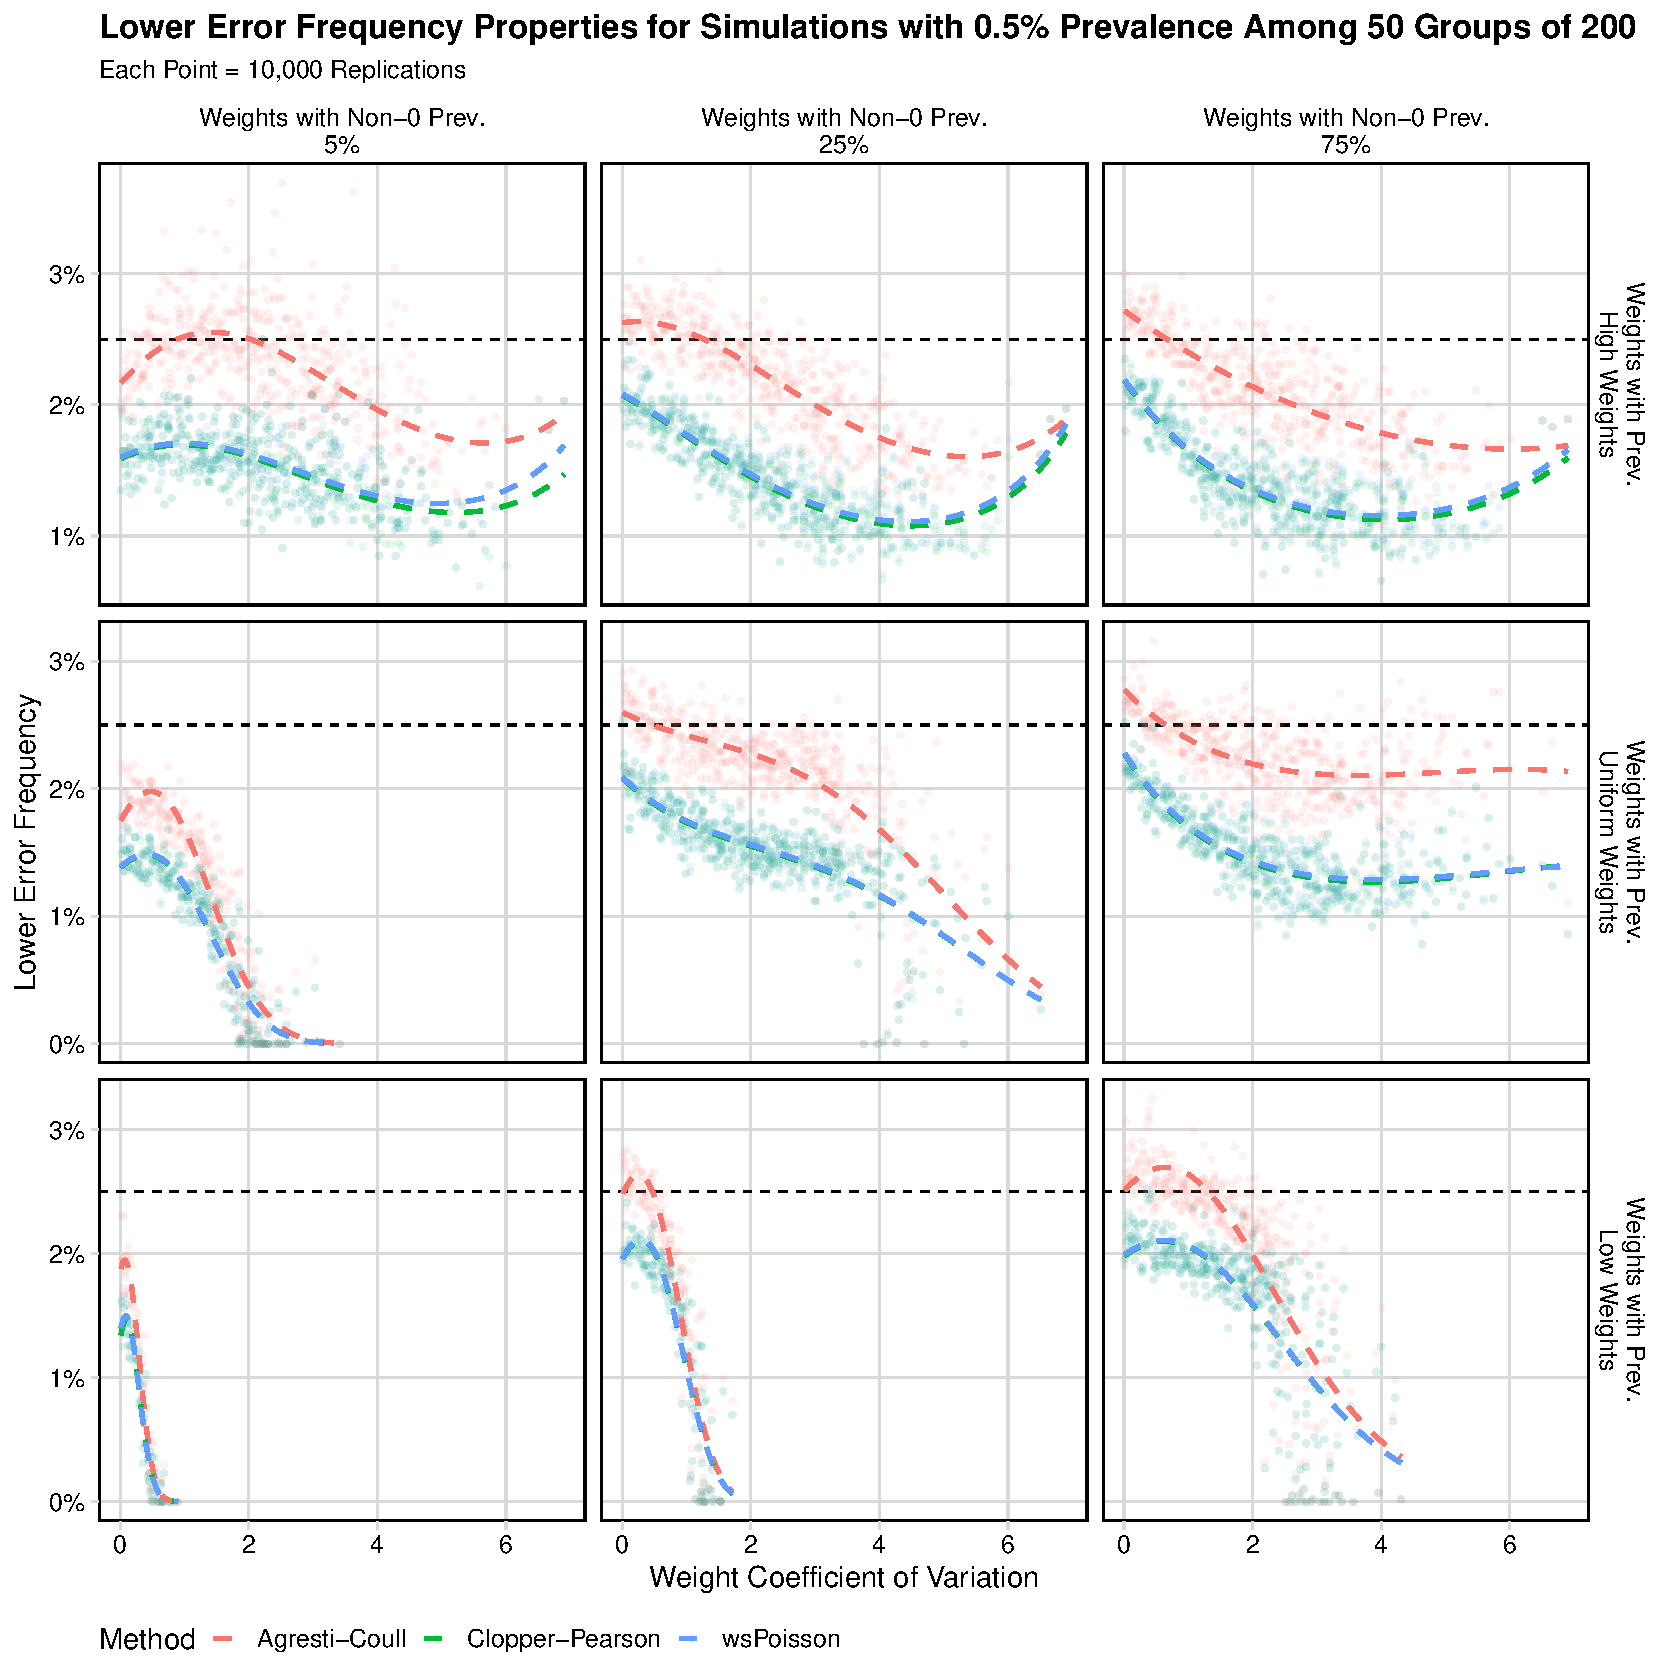
\includegraphics[width=\textwidth]{figures/perfect_lower_error_frequency_50_groups_0_005_prev.pdf}
\caption{Caption}
\label{fig:perfect_lower_error_frequency_50_groups_0_005_prev}
\end{figure}

\begin{figure}
\centering
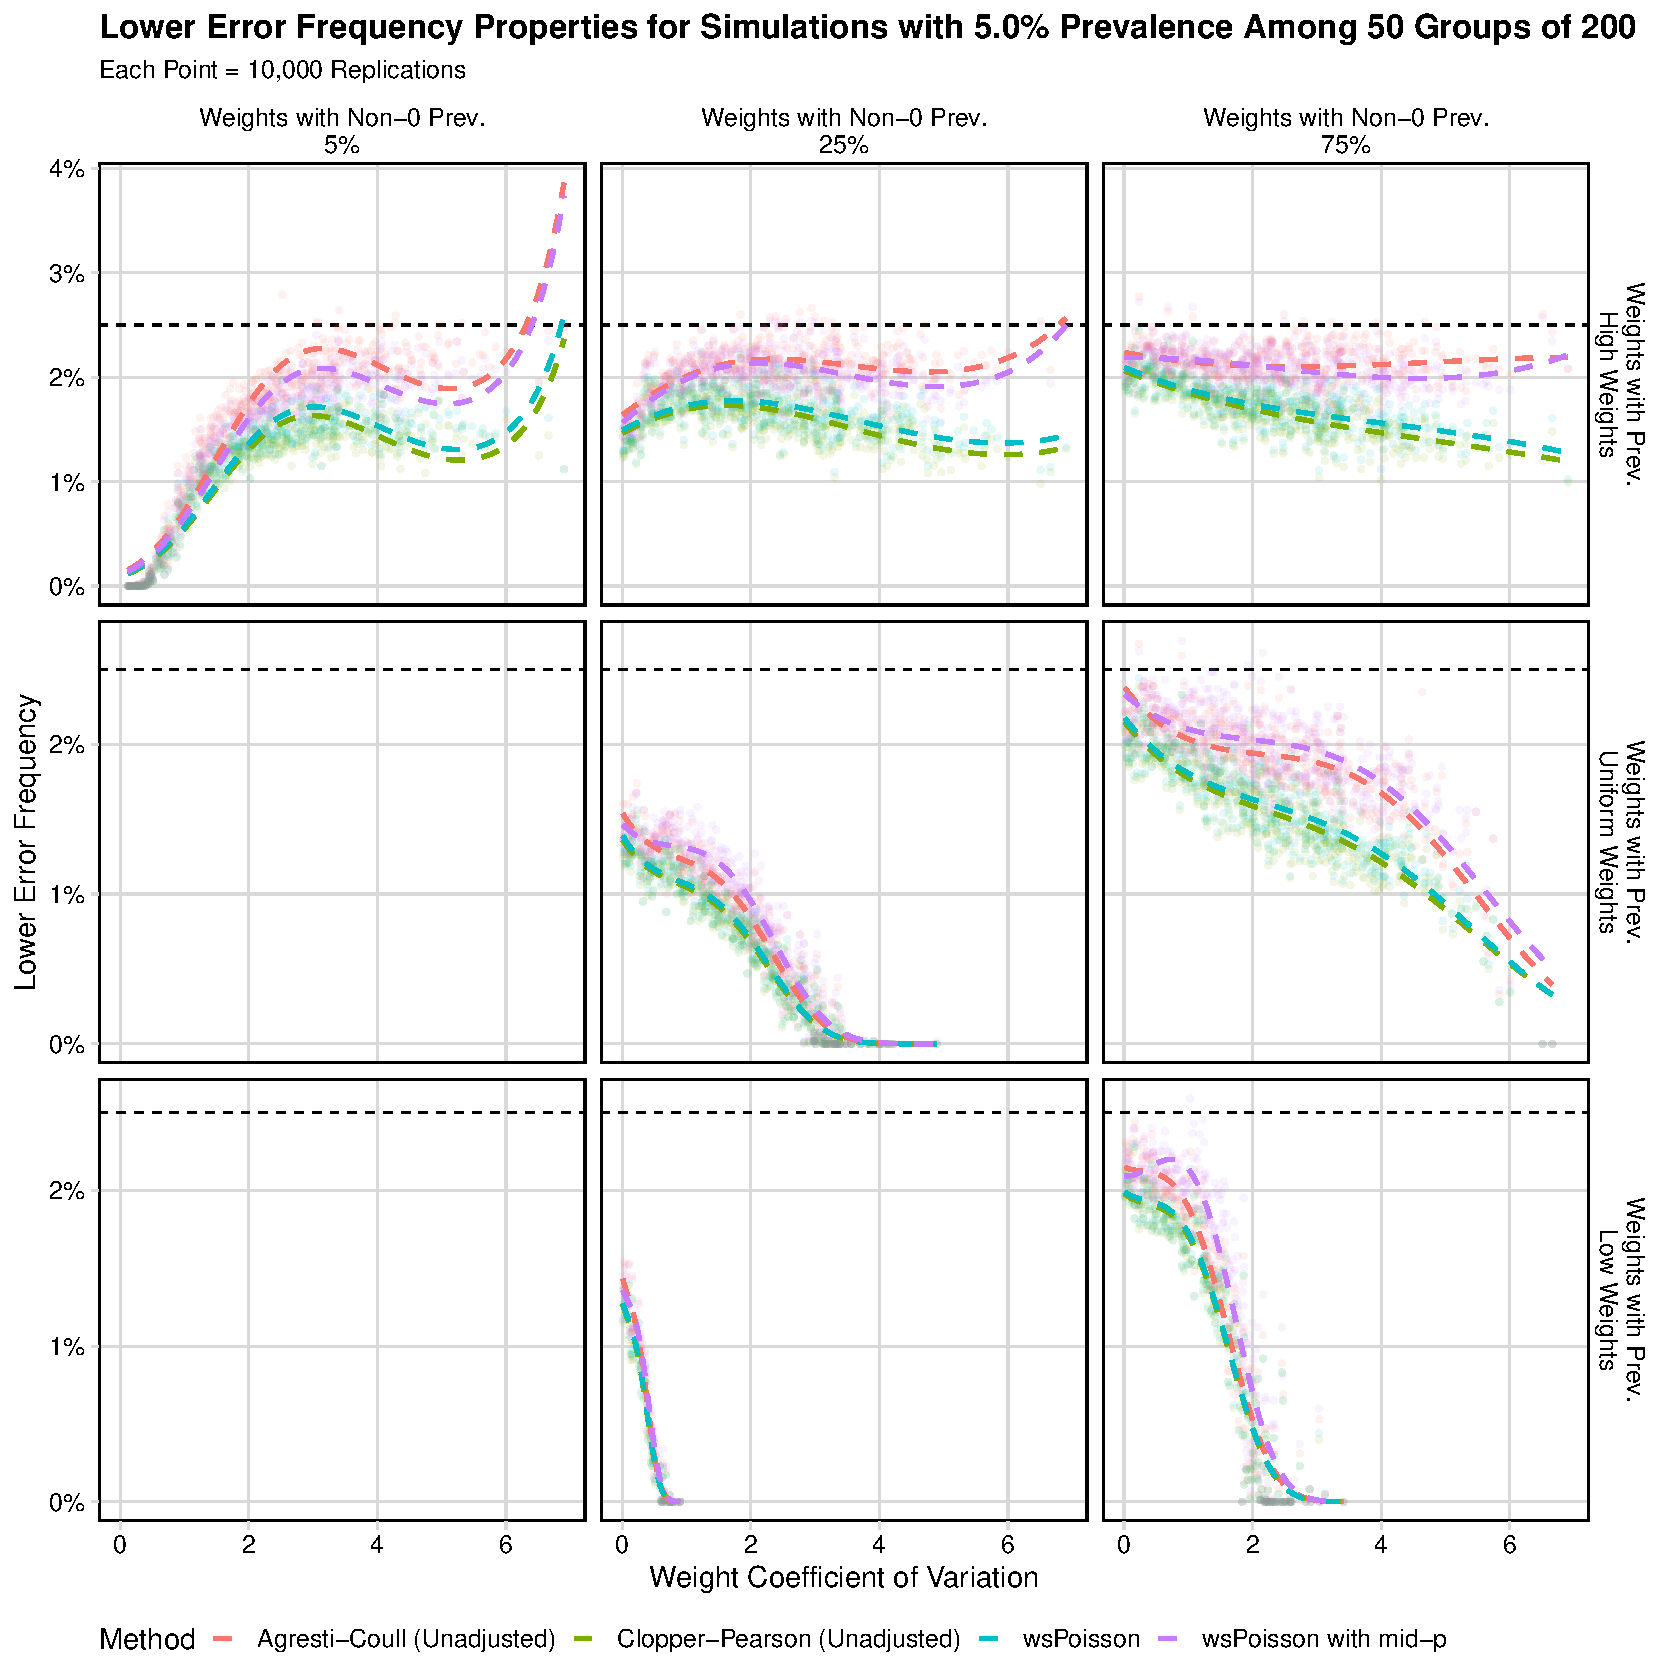
\includegraphics[width=\textwidth]{figures/perfect_lower_error_frequency_50_groups_0_05_prev.pdf}
\caption{Caption}
\label{fig:perfect_lower_error_frequency_50_groups_0_05_prev}
\end{figure}

\begin{figure}
\centering
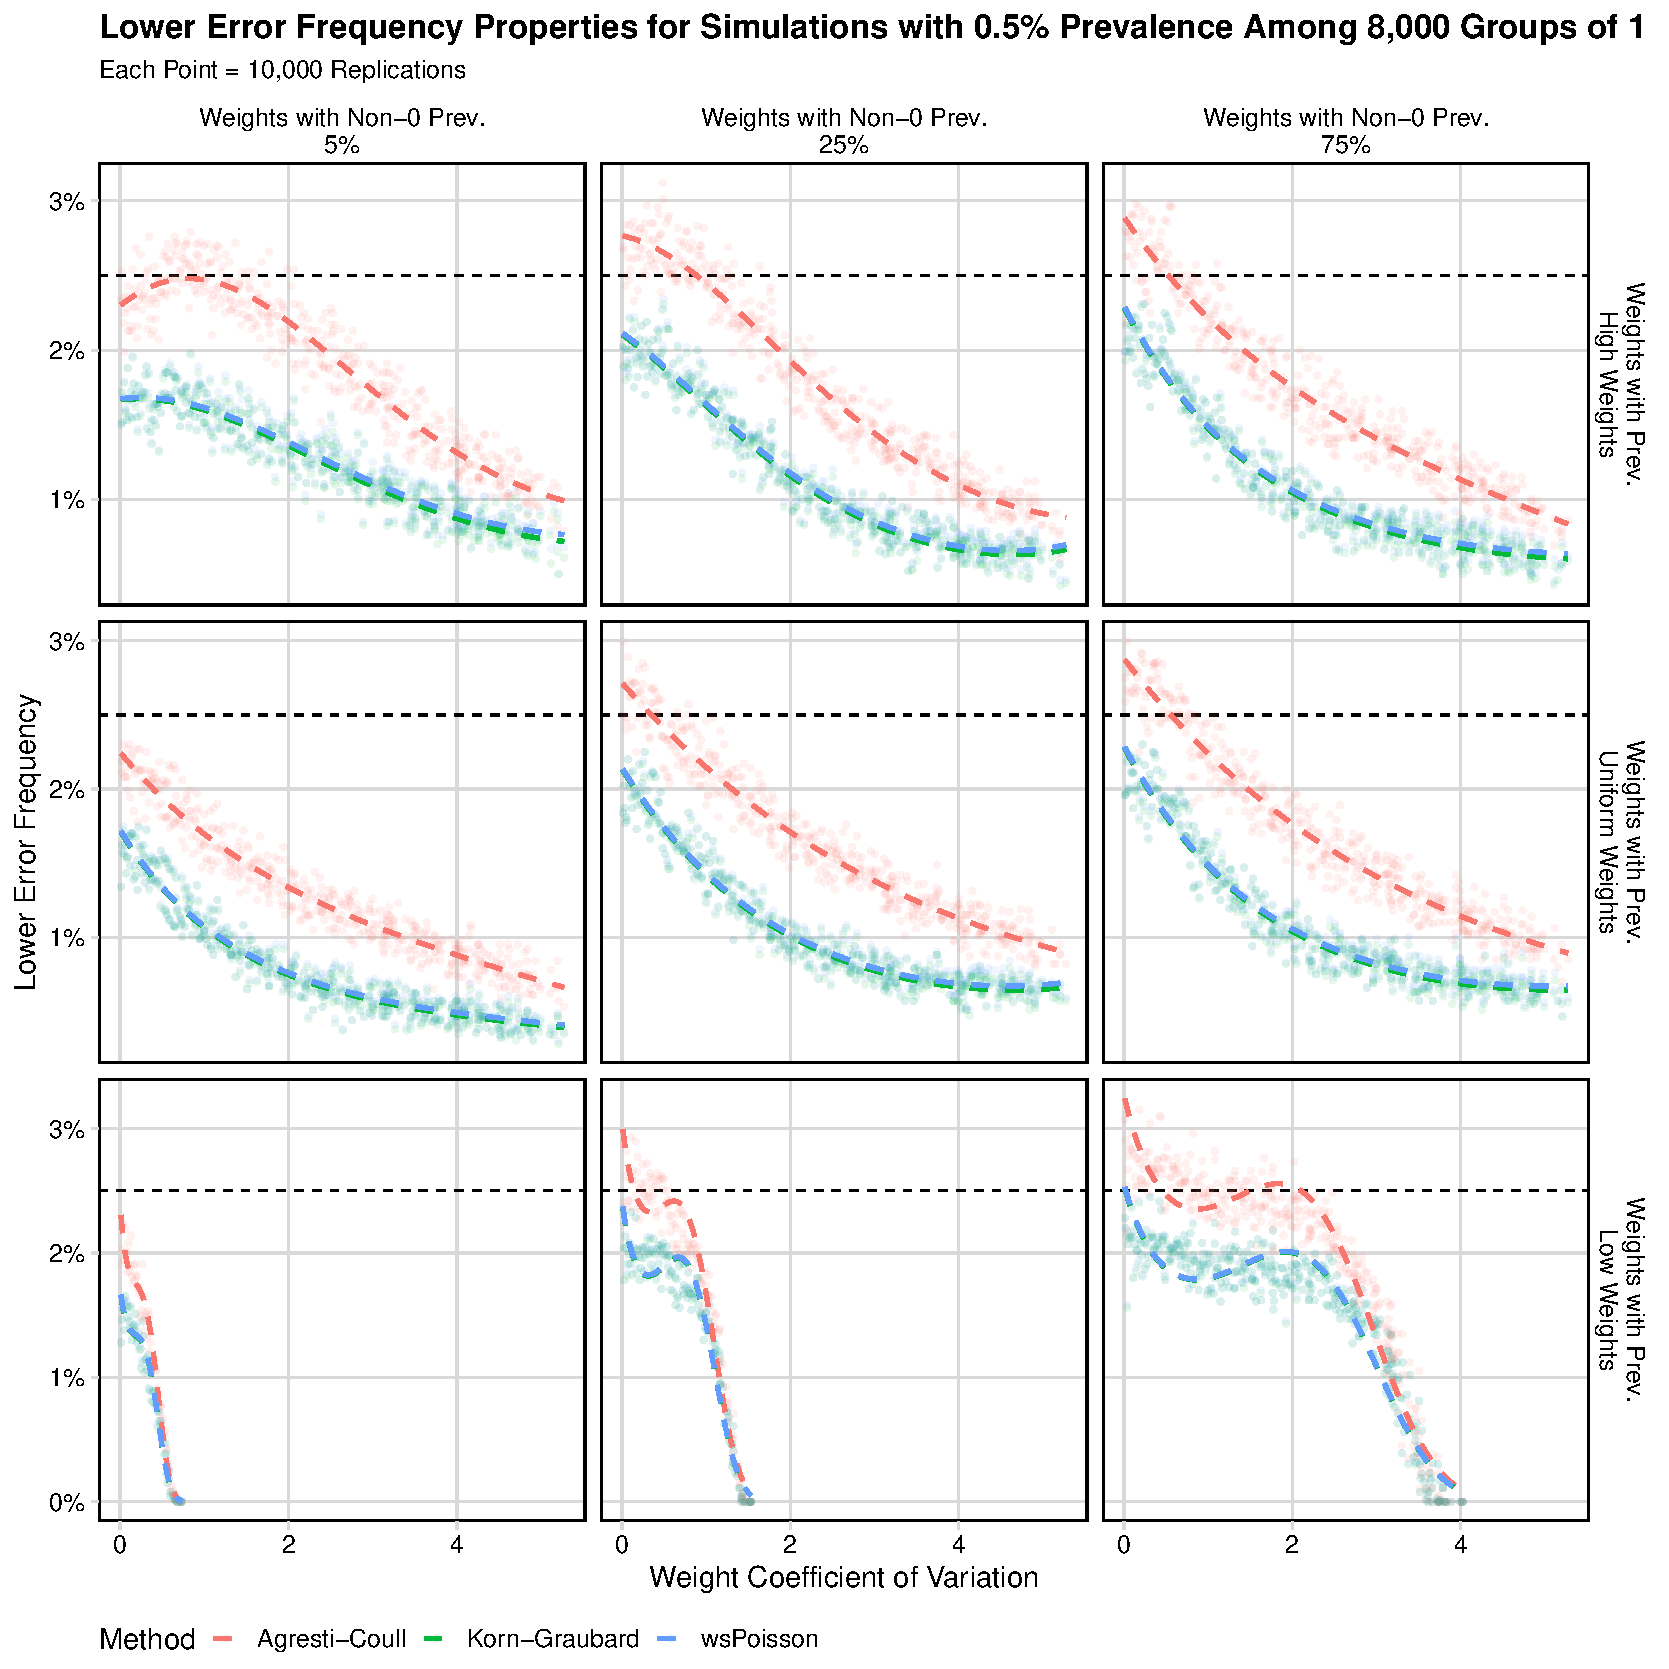
\includegraphics[width=\textwidth]{figures/perfect_lower_error_frequency_8000_groups_0_005_prev.pdf}
\caption{Caption}
\label{fig:perfect_lower_error_frequency_8000_groups_0_005_prev}
\end{figure}

\begin{figure}
\centering
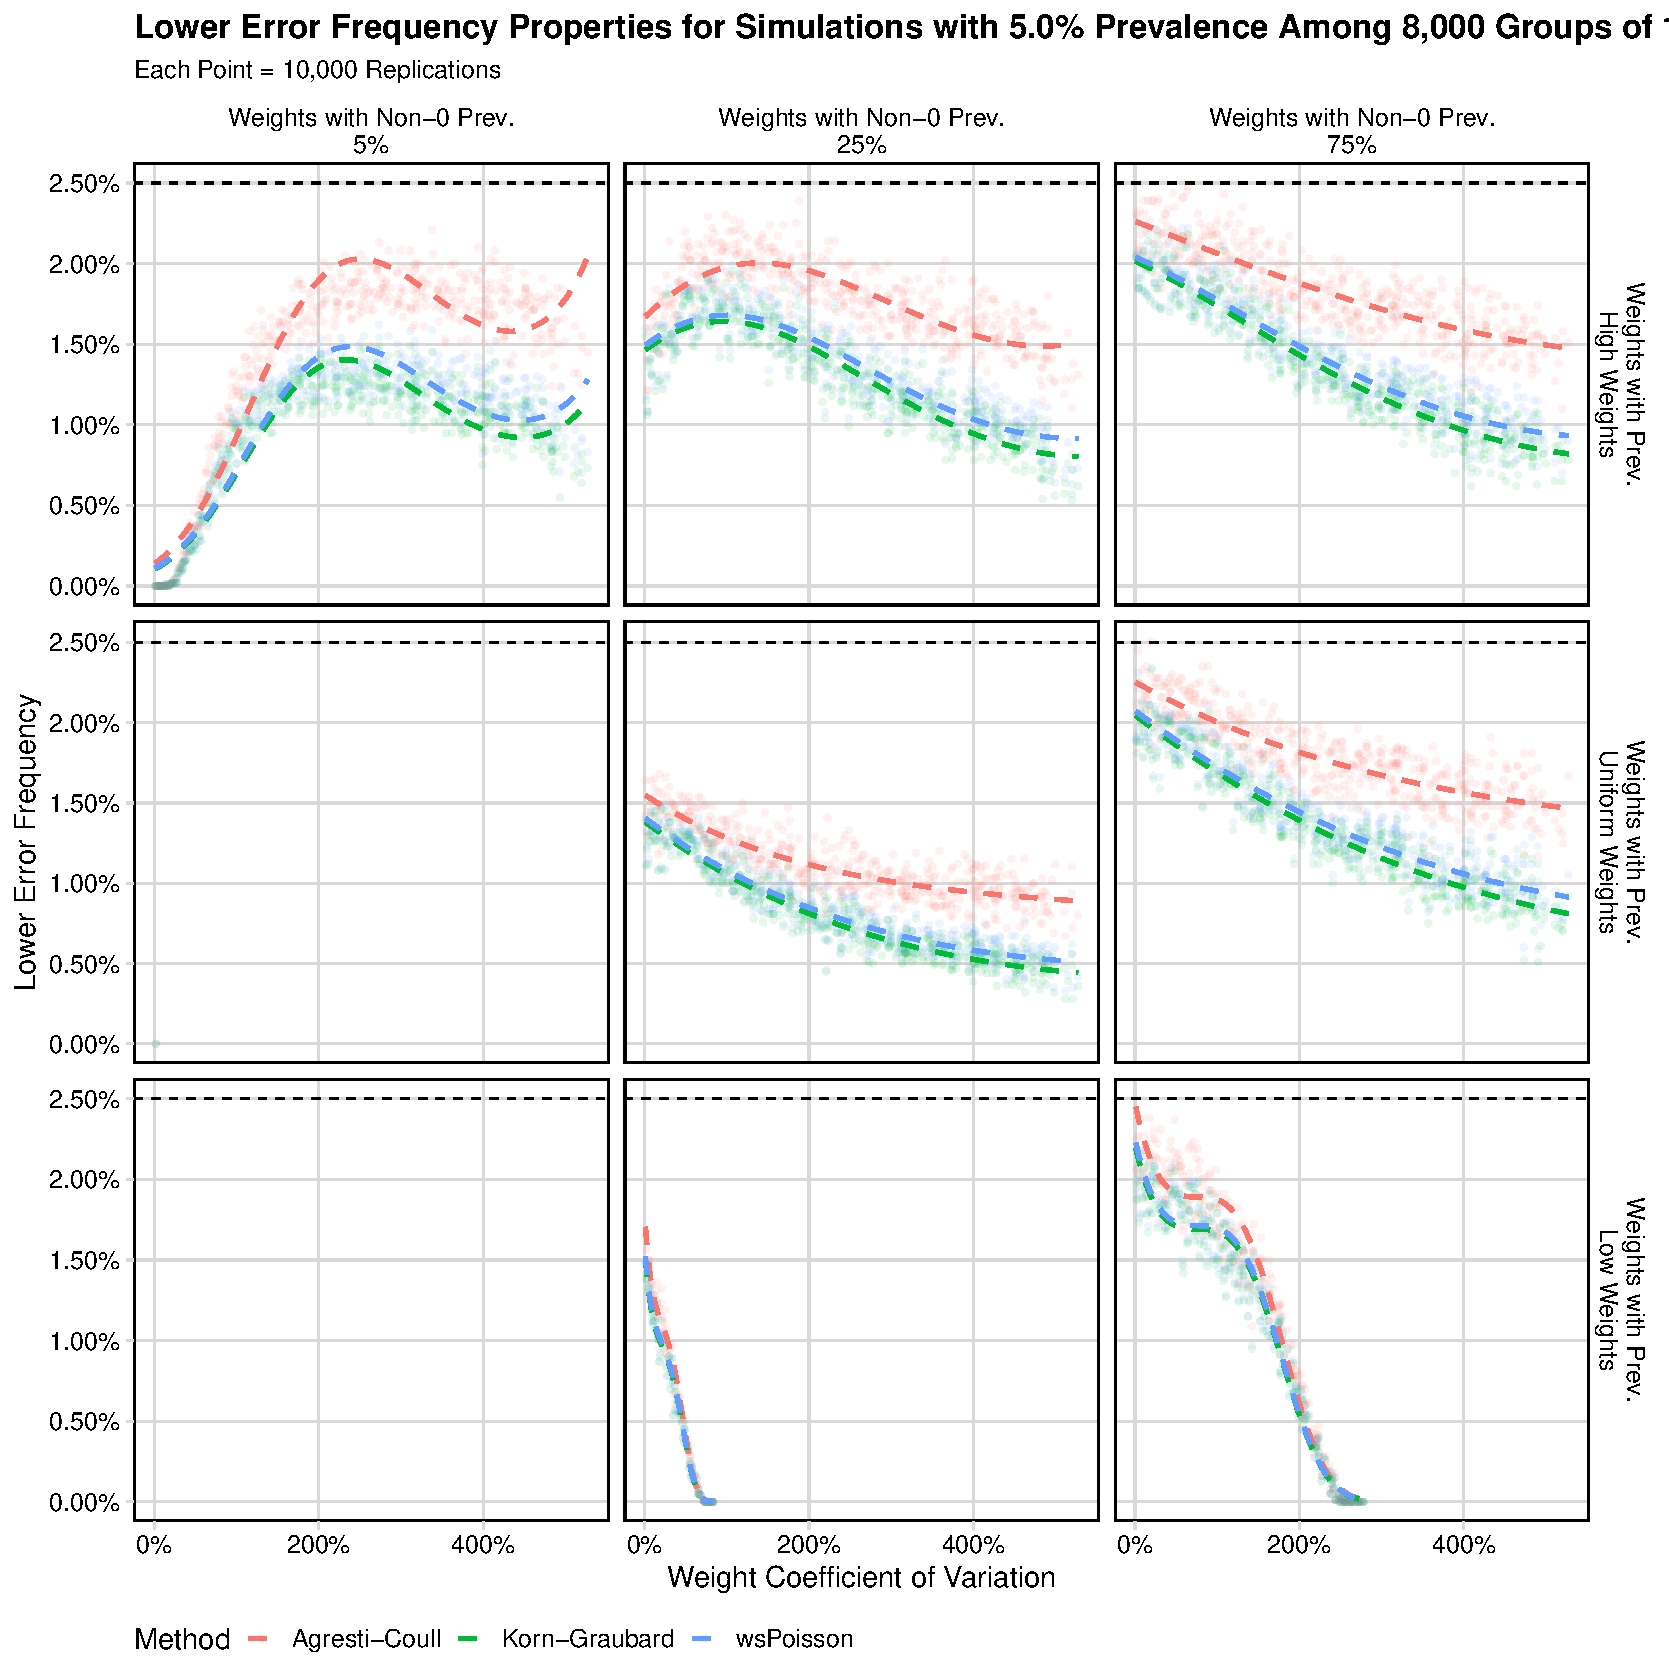
\includegraphics[width=\textwidth]{figures/perfect_lower_error_frequency_8000_groups_0_05_prev.pdf}
\caption{Caption}
\label{fig:perfect_lower_error_frequency_8000_groups_0_05_prev}
\end{figure}

\begin{figure}
\centering
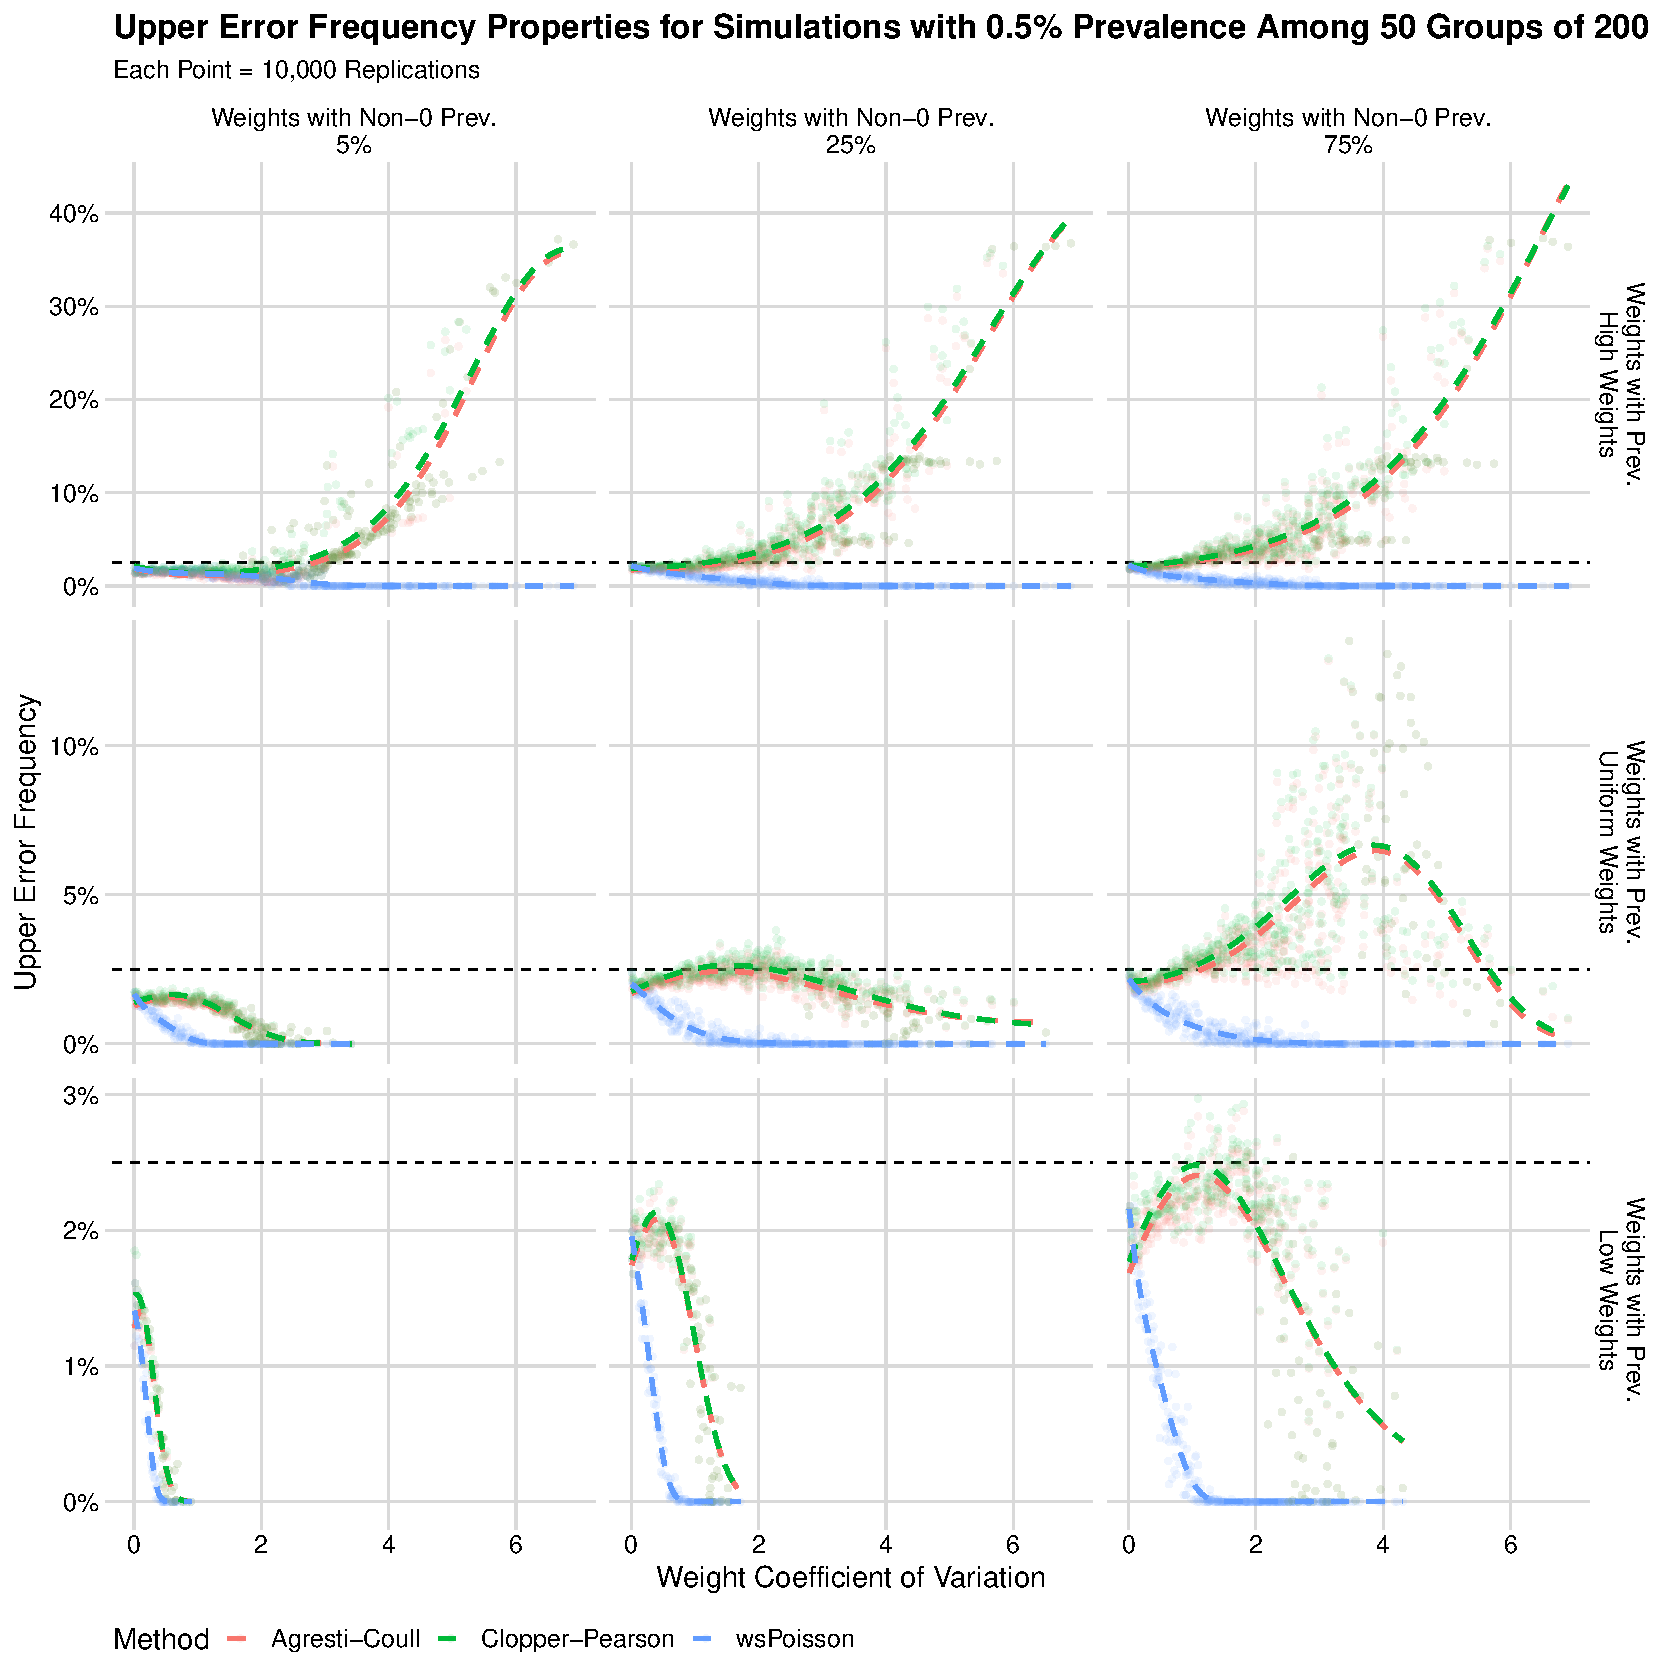
\includegraphics[width=\textwidth]{figures/perfect_upper_error_frequency_50_groups_0_005_prev.pdf}
\caption{Caption}
\label{fig:perfect_upper_error_frequency_50_groups_0_005_prev}
\end{figure}

\begin{figure}
\centering
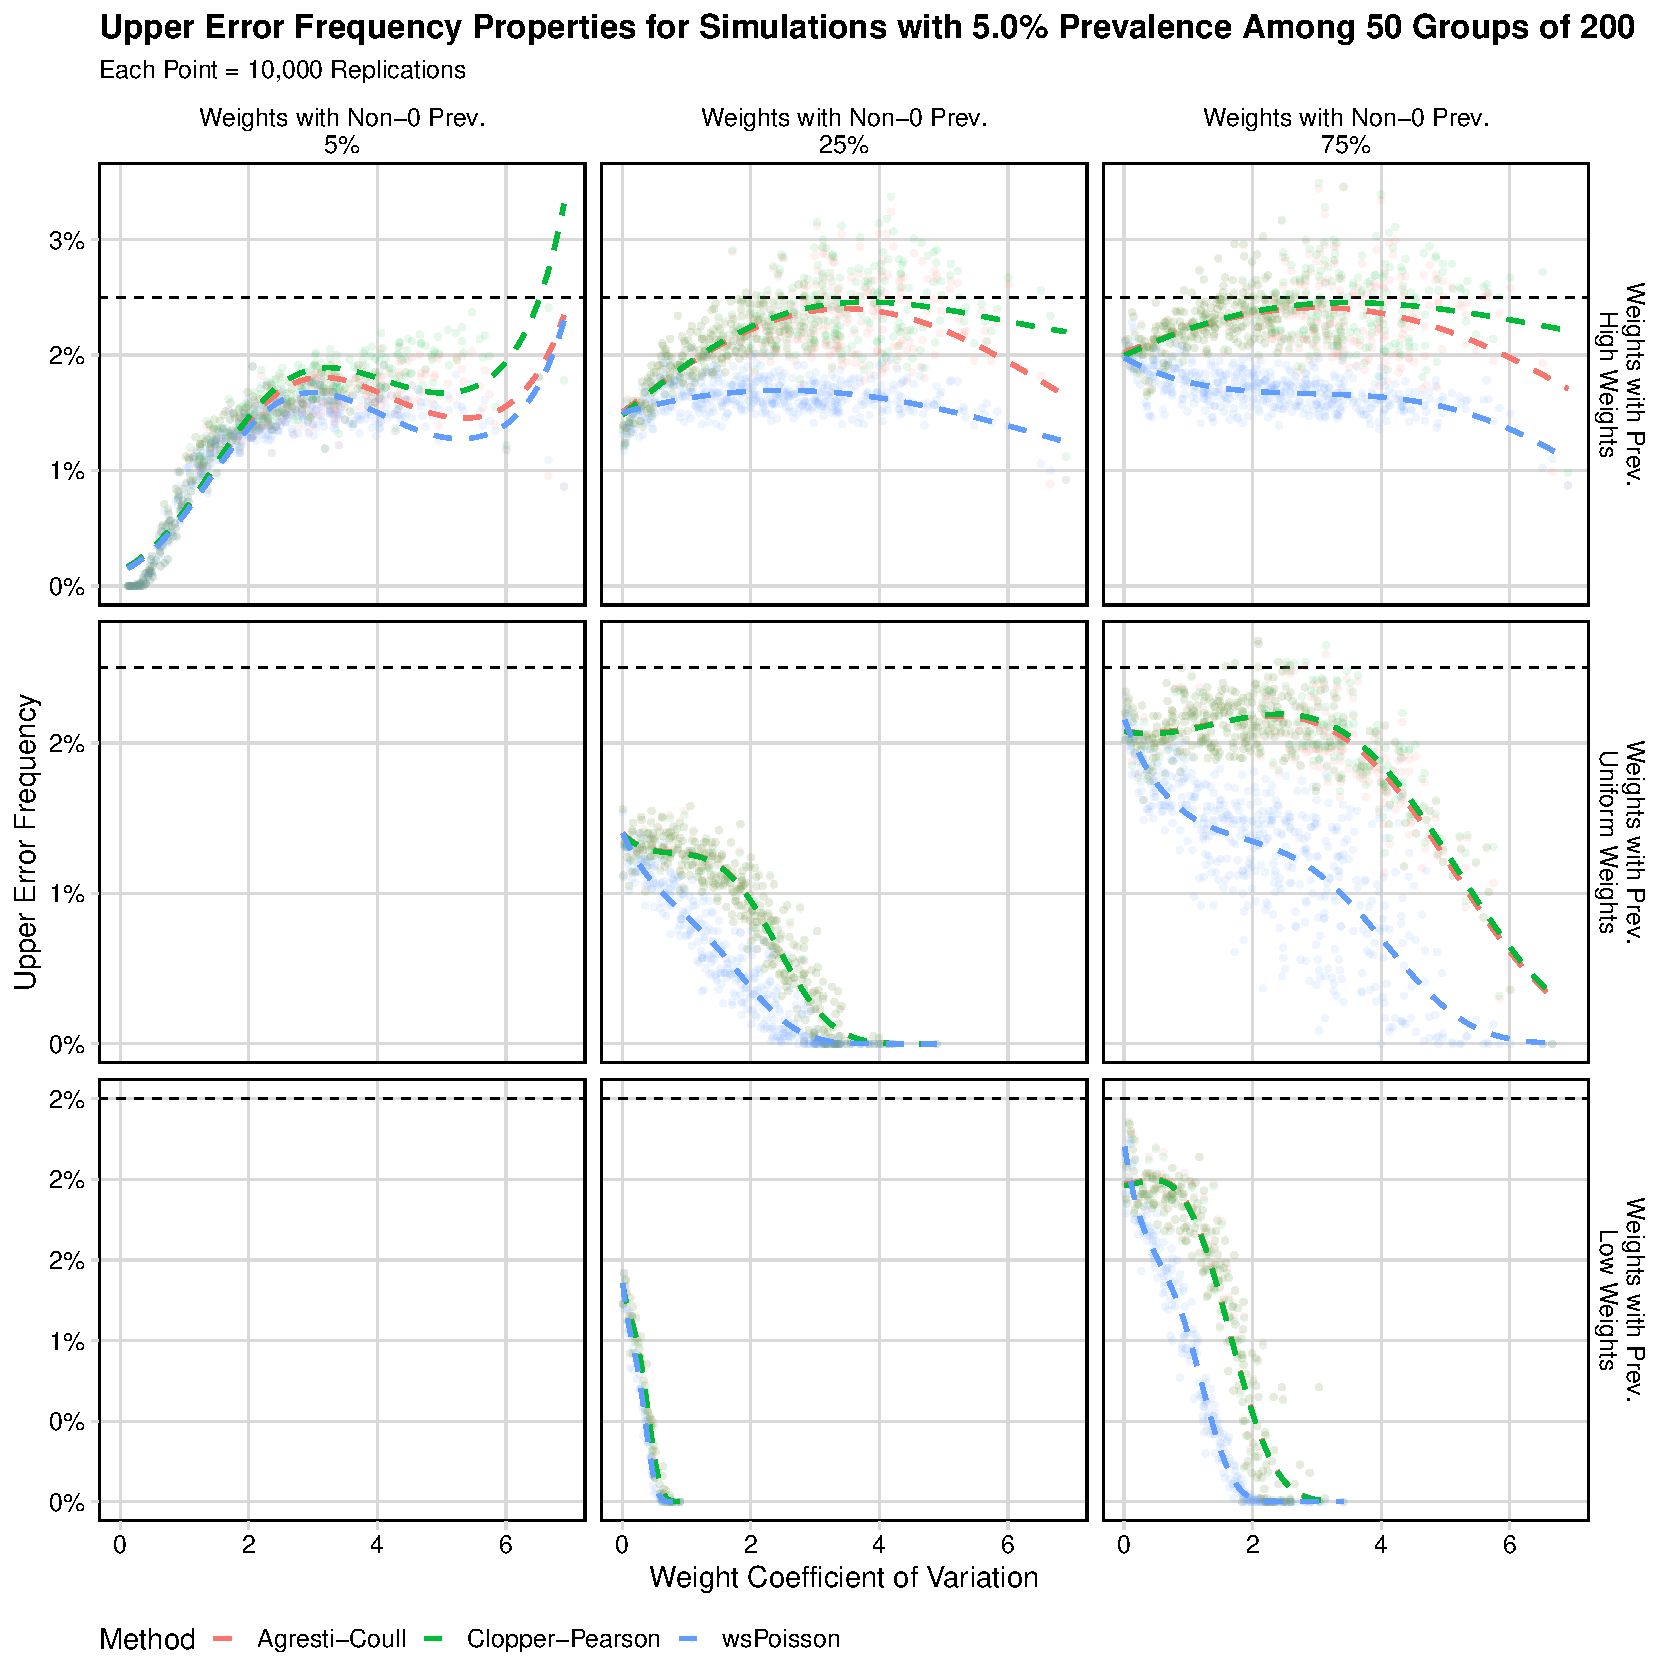
\includegraphics[width=\textwidth]{figures/perfect_upper_error_frequency_50_groups_0_05_prev.pdf}
\caption{Caption}
\label{fig:perfect_upper_error_frequency_50_groups_0_05_prev}
\end{figure}

\begin{figure}
\centering
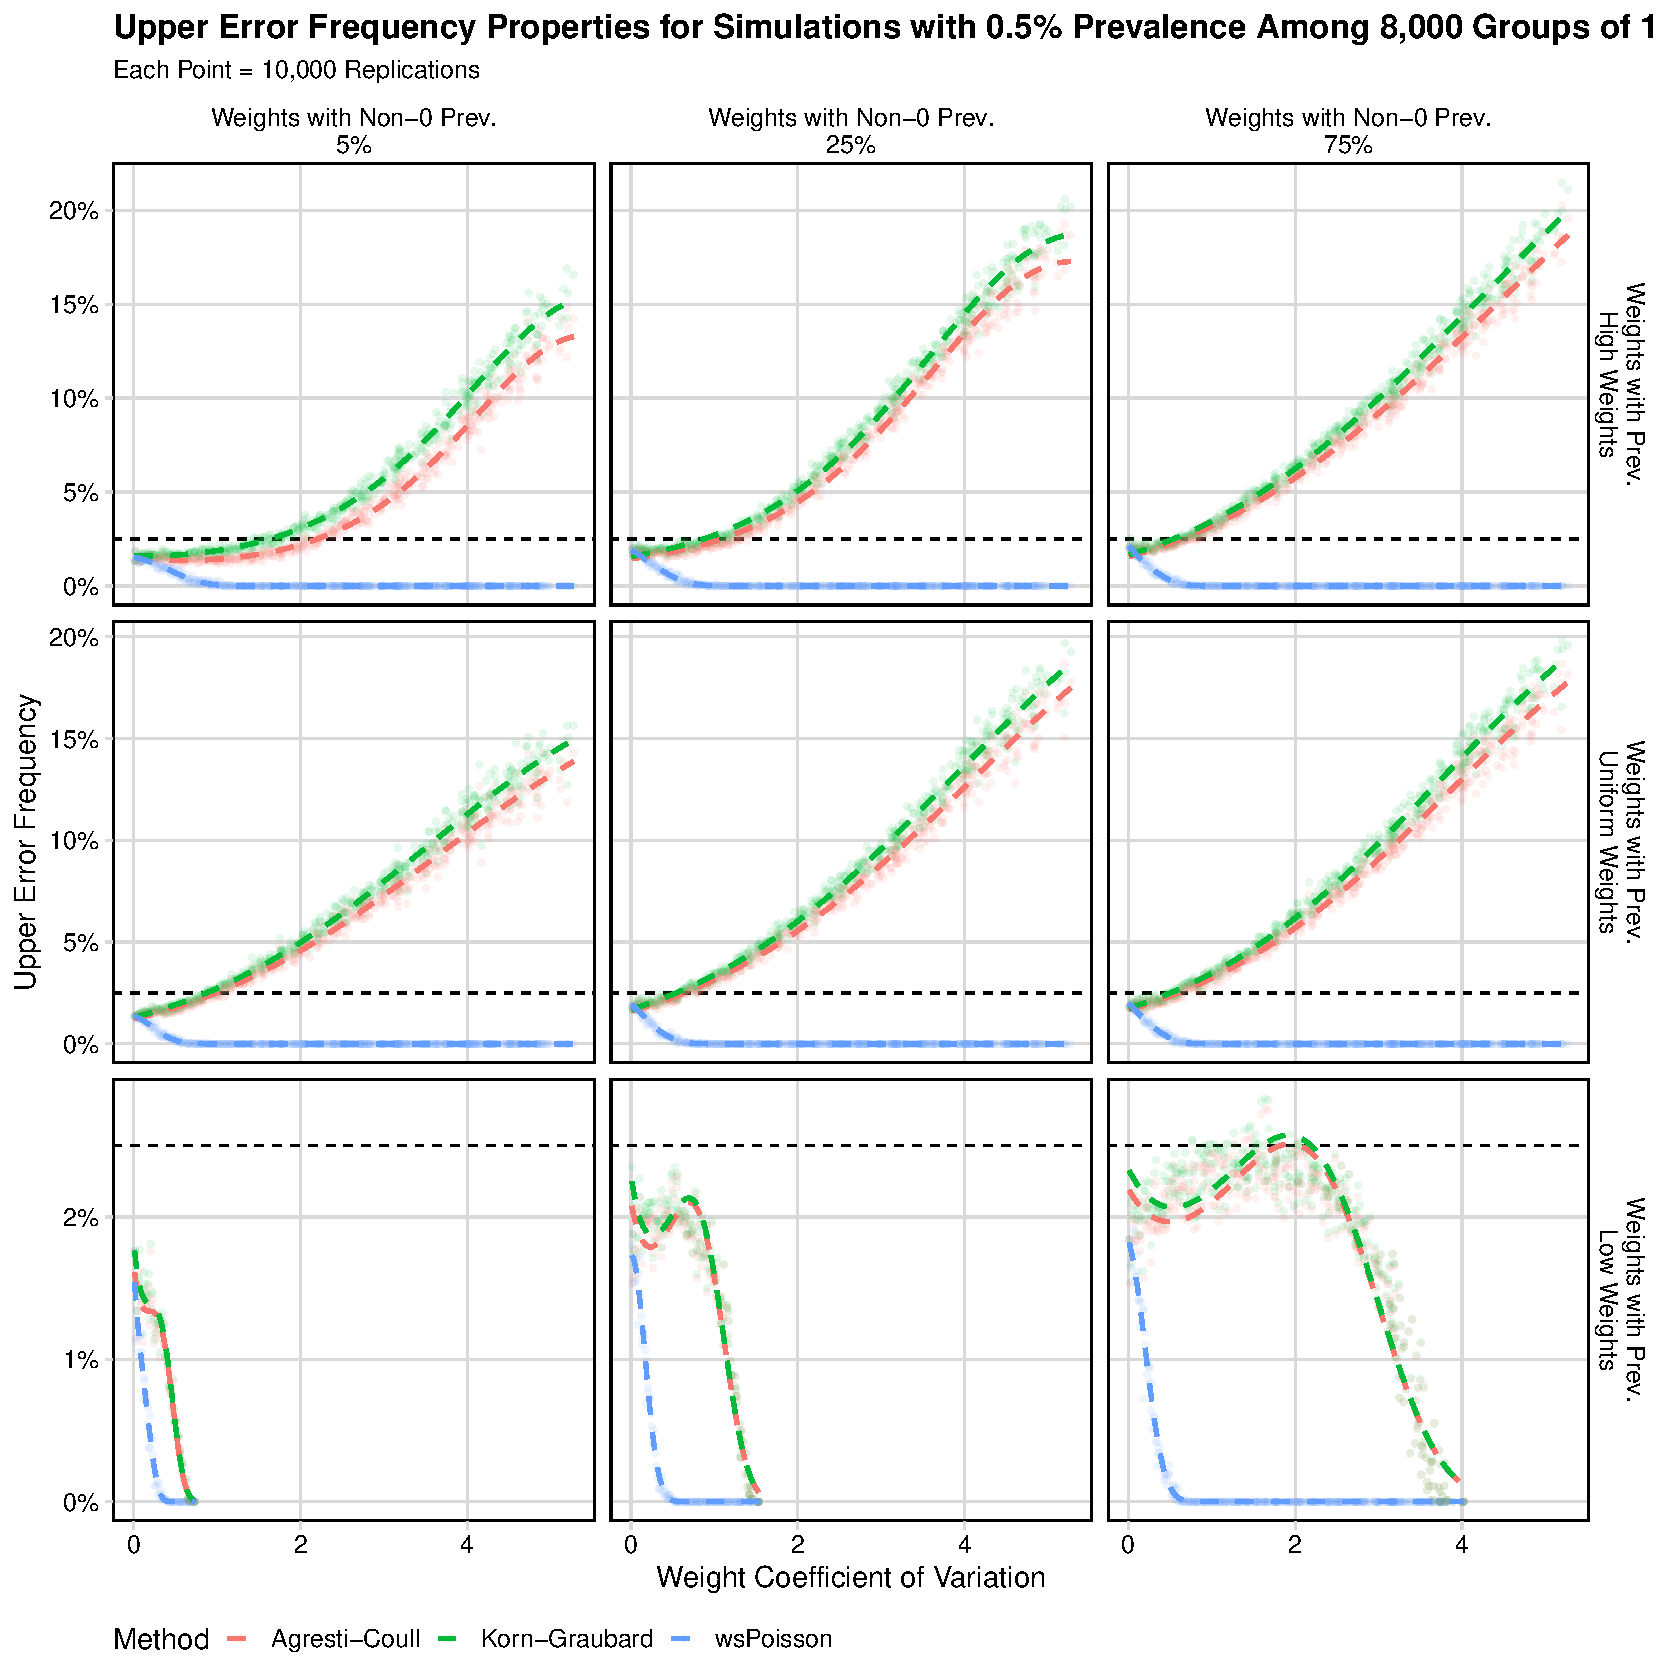
\includegraphics[width=\textwidth]{figures/perfect_upper_error_frequency_8000_groups_0_005_prev.pdf}
\caption{Caption}
\label{fig:perfect_upper_error_frequency_8000_groups_0_005_prev}
\end{figure}

\begin{figure}
\centering
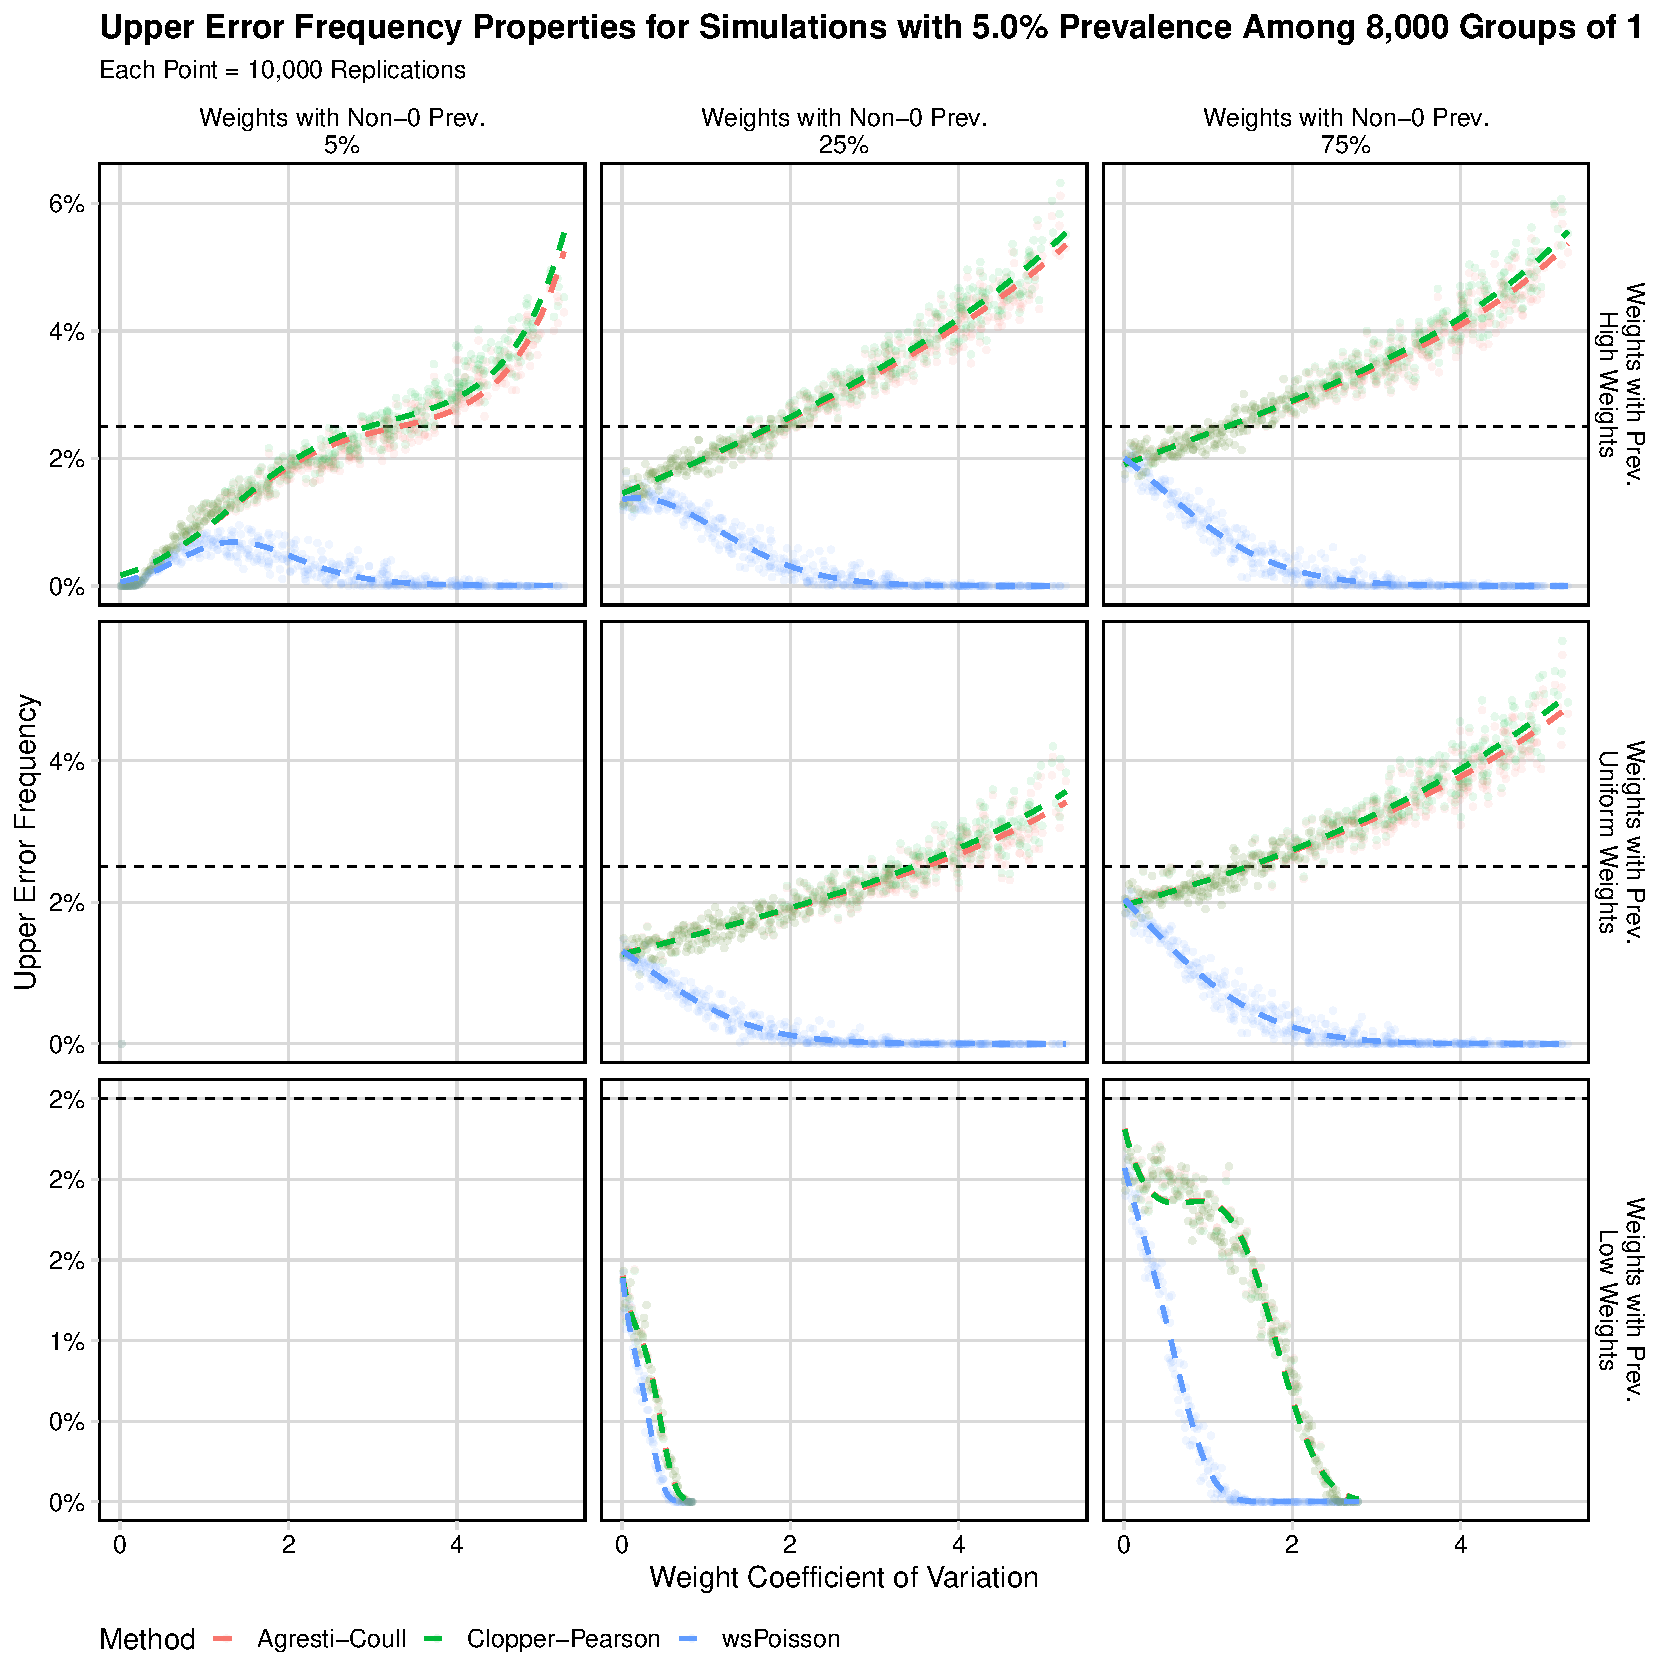
\includegraphics[width=\textwidth]{figures/perfect_upper_error_frequency_8000_groups_0_05_prev.pdf}
\caption{Caption}
\label{fig:perfect_upper_error_frequency_8000_groups_0_05_prev}
\end{figure}

\begin{figure}
\centering
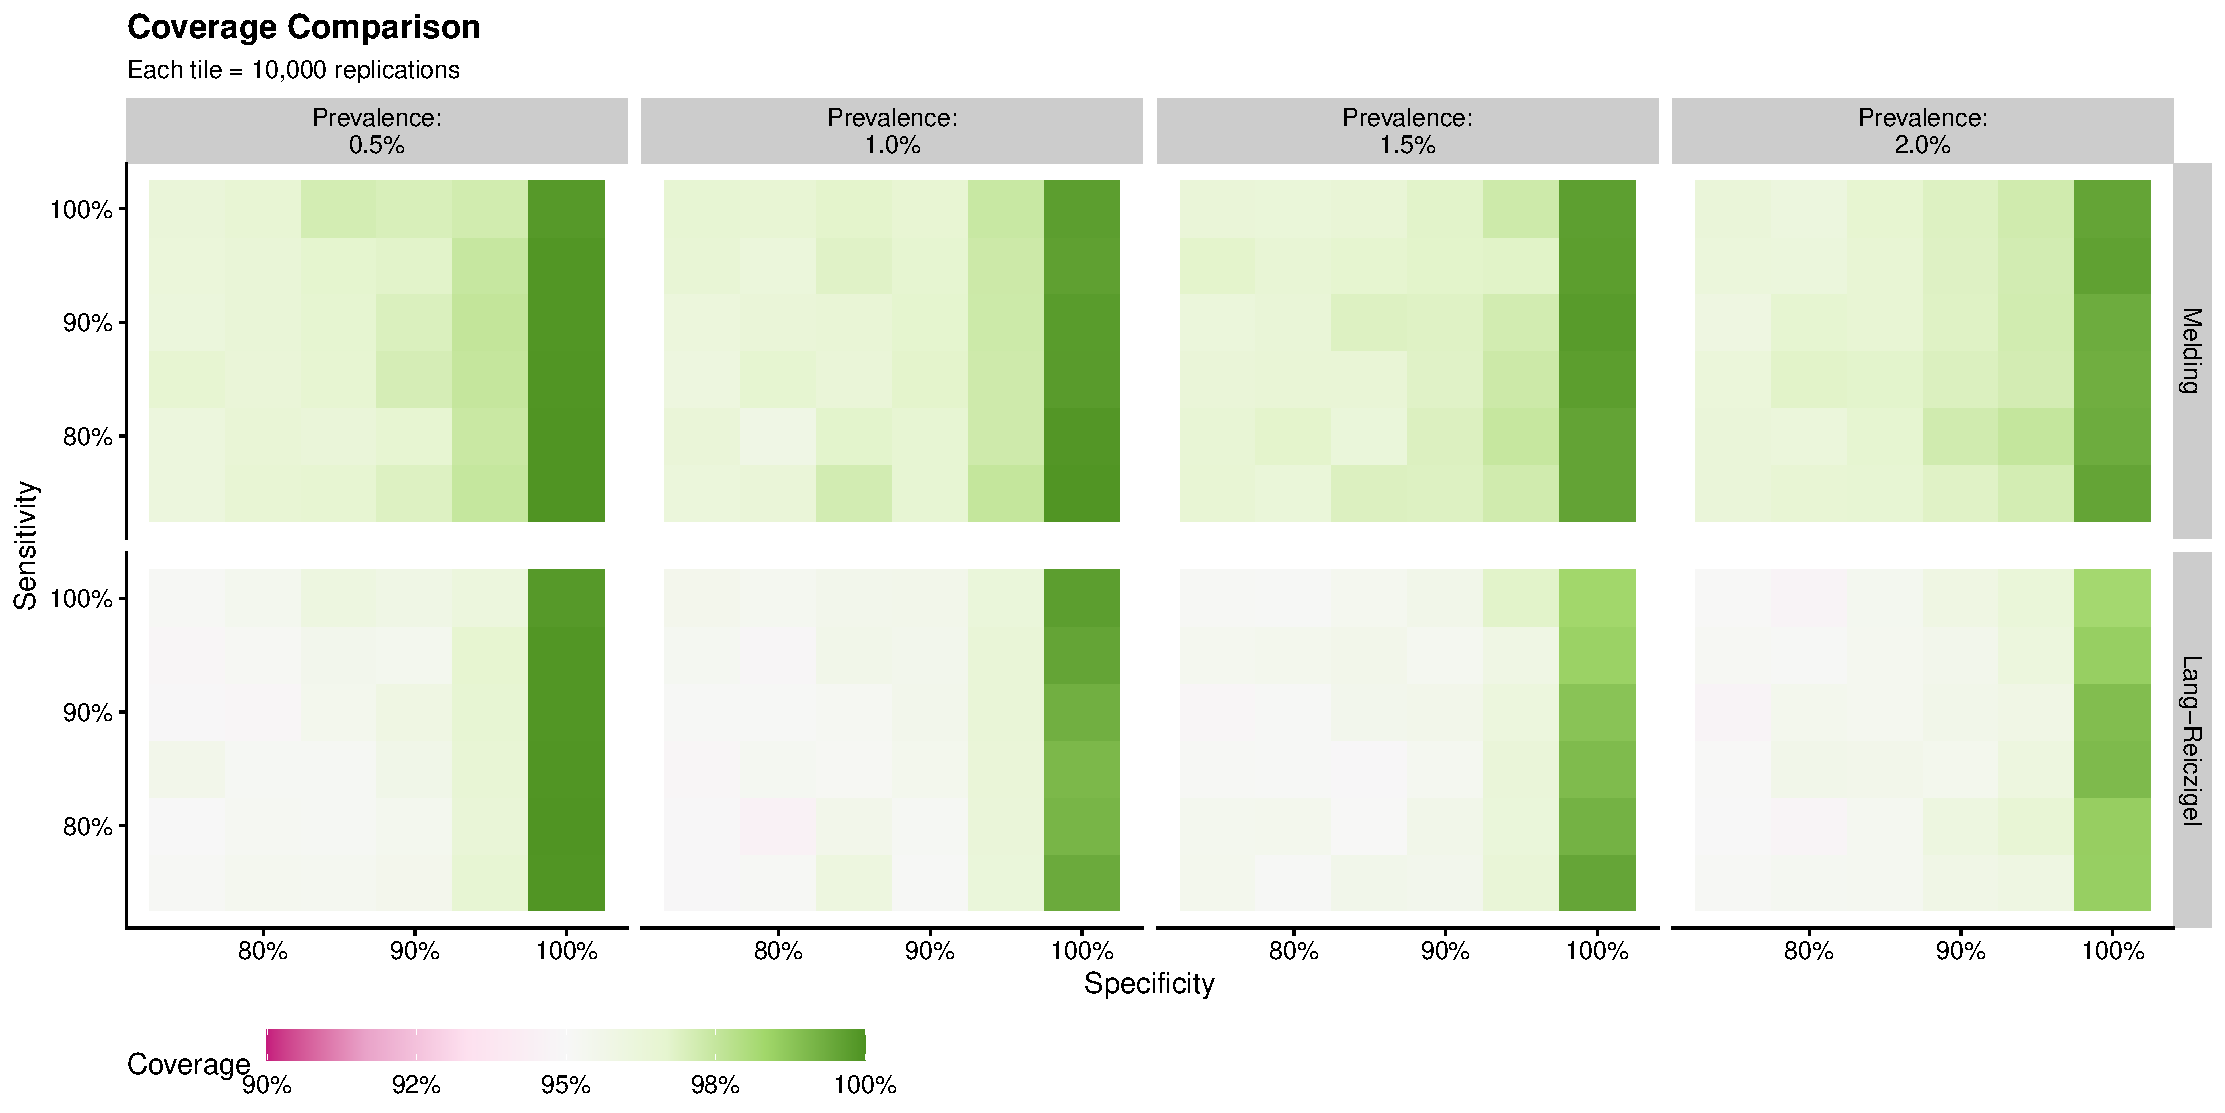
\includegraphics[width=\textwidth]{figures/simple_coverage_comparison_plot.pdf}
\caption{Caption}
\label{fig:simple_coverage_comparison_plot}
\end{figure}

\begin{figure}
\centering
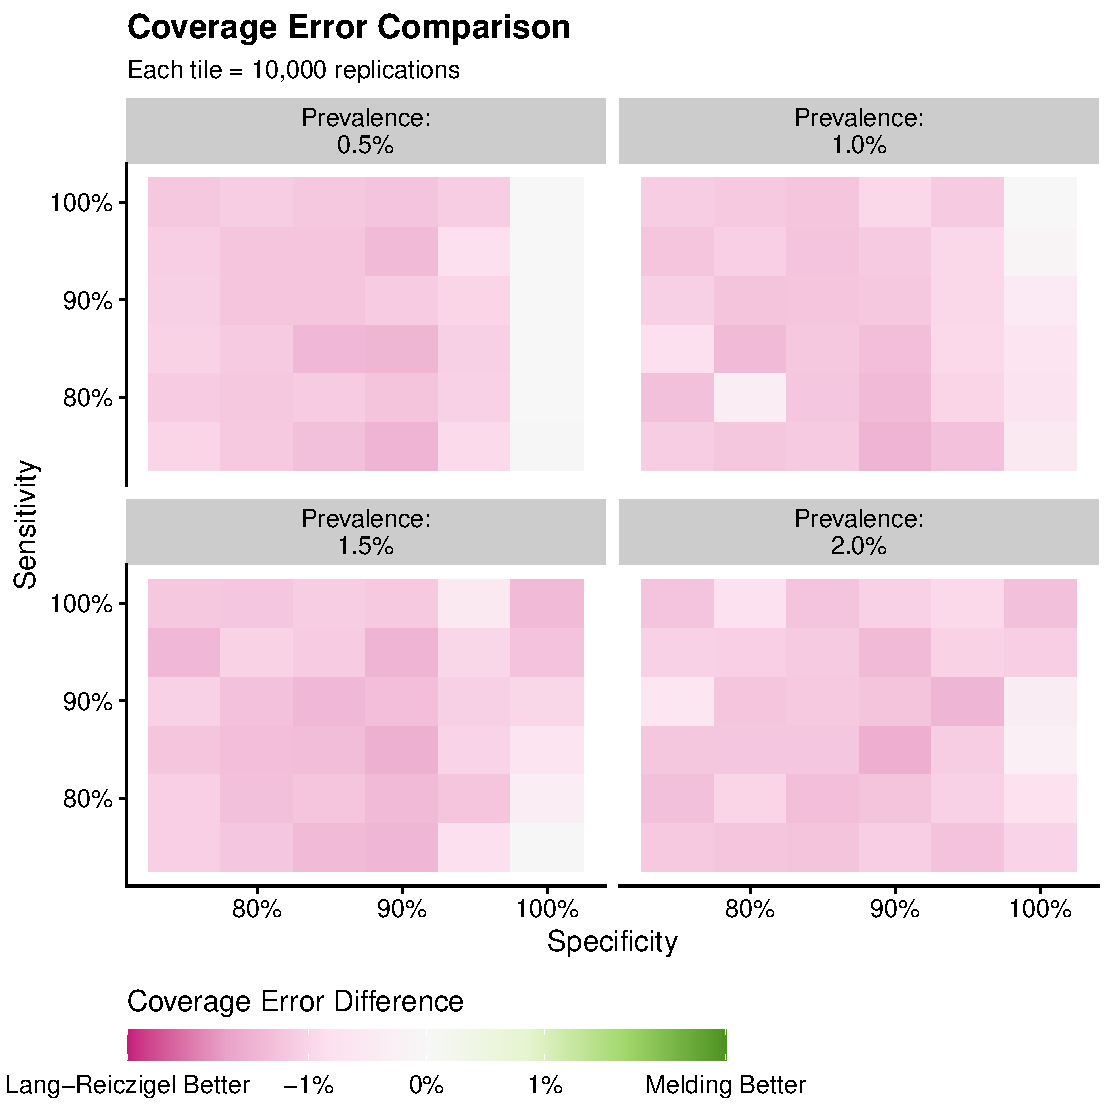
\includegraphics[width=\textwidth]{figures/simple_coverage_error_comparison_plot.pdf}
\caption{Caption}
\label{fig:simple_coverage_error_comparison_plot}
\end{figure}

\begin{figure}
\centering
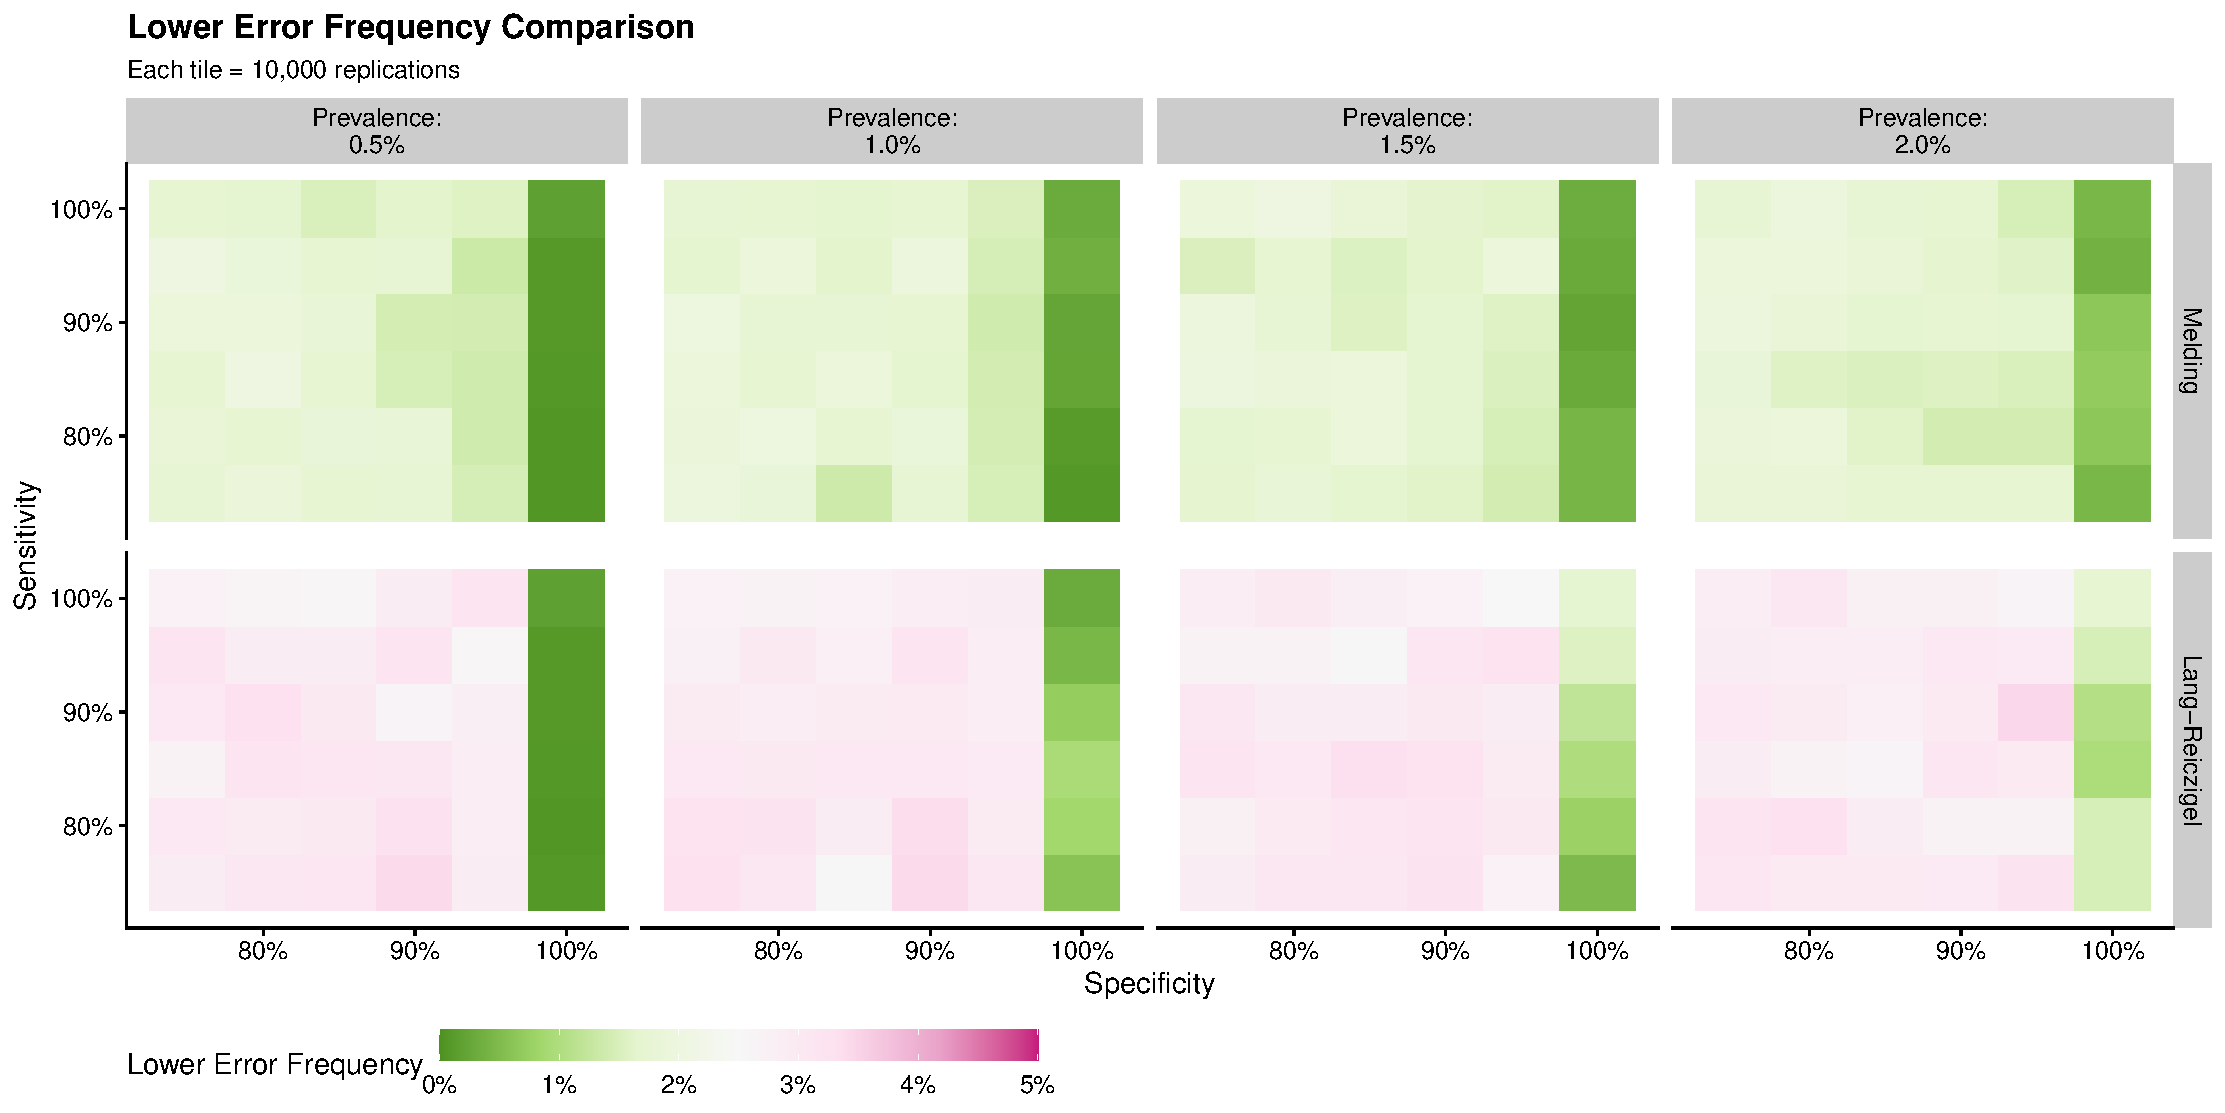
\includegraphics[width=\textwidth]{figures/simple_lower_error_frequency_comparison_plot.pdf}
\caption{Caption}
\label{fig:simple_lower_error_frequency_comparison_plot}
\end{figure}

\begin{figure}
\centering
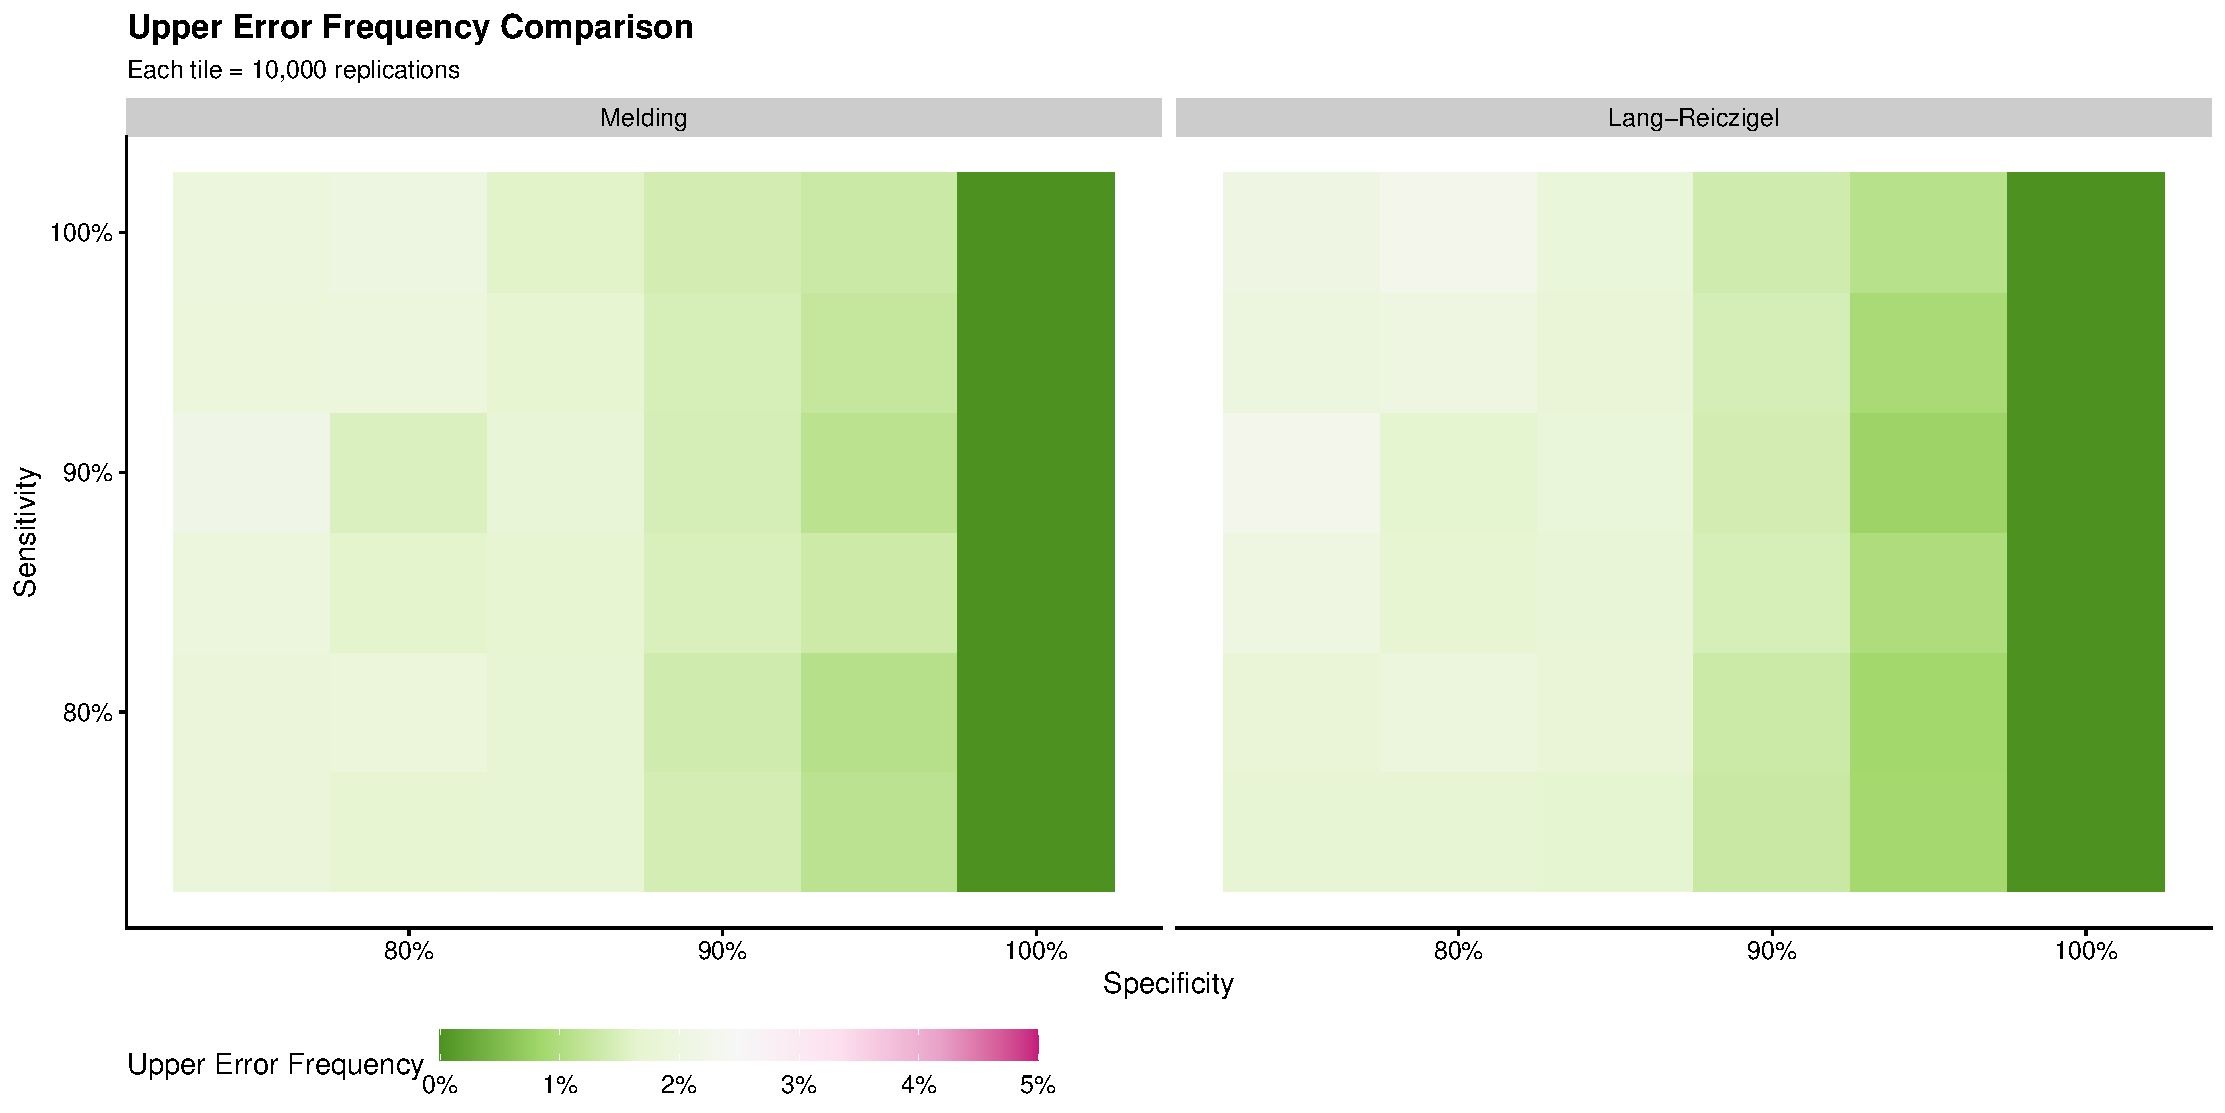
\includegraphics[width=\textwidth]{figures/simple_upper_error_frequency_comparison_plot.pdf}
\caption{Caption}
\label{fig:simple_upper_error_frequency_comparison_plot}
\end{figure}

\end{document}